% Options for packages loaded elsewhere
\PassOptionsToPackage{unicode}{hyperref}
\PassOptionsToPackage{hyphens}{url}
%
\documentclass[
]{book}
\usepackage{lmodern}
\usepackage{amssymb,amsmath}
\usepackage{ifxetex,ifluatex}
\ifnum 0\ifxetex 1\fi\ifluatex 1\fi=0 % if pdftex
  \usepackage[T1]{fontenc}
  \usepackage[utf8]{inputenc}
  \usepackage{textcomp} % provide euro and other symbols
\else % if luatex or xetex
  \usepackage{unicode-math}
  \defaultfontfeatures{Scale=MatchLowercase}
  \defaultfontfeatures[\rmfamily]{Ligatures=TeX,Scale=1}
\fi
% Use upquote if available, for straight quotes in verbatim environments
\IfFileExists{upquote.sty}{\usepackage{upquote}}{}
\IfFileExists{microtype.sty}{% use microtype if available
  \usepackage[]{microtype}
  \UseMicrotypeSet[protrusion]{basicmath} % disable protrusion for tt fonts
}{}
\makeatletter
\@ifundefined{KOMAClassName}{% if non-KOMA class
  \IfFileExists{parskip.sty}{%
    \usepackage{parskip}
  }{% else
    \setlength{\parindent}{0pt}
    \setlength{\parskip}{6pt plus 2pt minus 1pt}}
}{% if KOMA class
  \KOMAoptions{parskip=half}}
\makeatother
\usepackage{xcolor}
\IfFileExists{xurl.sty}{\usepackage{xurl}}{} % add URL line breaks if available
\IfFileExists{bookmark.sty}{\usepackage{bookmark}}{\usepackage{hyperref}}
\hypersetup{
  pdftitle={R 資料科學與統計},
  pdfauthor={Jeff Lin},
  hidelinks,
  pdfcreator={LaTeX via pandoc}}
\urlstyle{same} % disable monospaced font for URLs
\usepackage{color}
\usepackage{fancyvrb}
\newcommand{\VerbBar}{|}
\newcommand{\VERB}{\Verb[commandchars=\\\{\}]}
\DefineVerbatimEnvironment{Highlighting}{Verbatim}{commandchars=\\\{\}}
% Add ',fontsize=\small' for more characters per line
\usepackage{framed}
\definecolor{shadecolor}{RGB}{248,248,248}
\newenvironment{Shaded}{\begin{snugshade}}{\end{snugshade}}
\newcommand{\AlertTok}[1]{\textcolor[rgb]{0.94,0.16,0.16}{#1}}
\newcommand{\AnnotationTok}[1]{\textcolor[rgb]{0.56,0.35,0.01}{\textbf{\textit{#1}}}}
\newcommand{\AttributeTok}[1]{\textcolor[rgb]{0.77,0.63,0.00}{#1}}
\newcommand{\BaseNTok}[1]{\textcolor[rgb]{0.00,0.00,0.81}{#1}}
\newcommand{\BuiltInTok}[1]{#1}
\newcommand{\CharTok}[1]{\textcolor[rgb]{0.31,0.60,0.02}{#1}}
\newcommand{\CommentTok}[1]{\textcolor[rgb]{0.56,0.35,0.01}{\textit{#1}}}
\newcommand{\CommentVarTok}[1]{\textcolor[rgb]{0.56,0.35,0.01}{\textbf{\textit{#1}}}}
\newcommand{\ConstantTok}[1]{\textcolor[rgb]{0.00,0.00,0.00}{#1}}
\newcommand{\ControlFlowTok}[1]{\textcolor[rgb]{0.13,0.29,0.53}{\textbf{#1}}}
\newcommand{\DataTypeTok}[1]{\textcolor[rgb]{0.13,0.29,0.53}{#1}}
\newcommand{\DecValTok}[1]{\textcolor[rgb]{0.00,0.00,0.81}{#1}}
\newcommand{\DocumentationTok}[1]{\textcolor[rgb]{0.56,0.35,0.01}{\textbf{\textit{#1}}}}
\newcommand{\ErrorTok}[1]{\textcolor[rgb]{0.64,0.00,0.00}{\textbf{#1}}}
\newcommand{\ExtensionTok}[1]{#1}
\newcommand{\FloatTok}[1]{\textcolor[rgb]{0.00,0.00,0.81}{#1}}
\newcommand{\FunctionTok}[1]{\textcolor[rgb]{0.00,0.00,0.00}{#1}}
\newcommand{\ImportTok}[1]{#1}
\newcommand{\InformationTok}[1]{\textcolor[rgb]{0.56,0.35,0.01}{\textbf{\textit{#1}}}}
\newcommand{\KeywordTok}[1]{\textcolor[rgb]{0.13,0.29,0.53}{\textbf{#1}}}
\newcommand{\NormalTok}[1]{#1}
\newcommand{\OperatorTok}[1]{\textcolor[rgb]{0.81,0.36,0.00}{\textbf{#1}}}
\newcommand{\OtherTok}[1]{\textcolor[rgb]{0.56,0.35,0.01}{#1}}
\newcommand{\PreprocessorTok}[1]{\textcolor[rgb]{0.56,0.35,0.01}{\textit{#1}}}
\newcommand{\RegionMarkerTok}[1]{#1}
\newcommand{\SpecialCharTok}[1]{\textcolor[rgb]{0.00,0.00,0.00}{#1}}
\newcommand{\SpecialStringTok}[1]{\textcolor[rgb]{0.31,0.60,0.02}{#1}}
\newcommand{\StringTok}[1]{\textcolor[rgb]{0.31,0.60,0.02}{#1}}
\newcommand{\VariableTok}[1]{\textcolor[rgb]{0.00,0.00,0.00}{#1}}
\newcommand{\VerbatimStringTok}[1]{\textcolor[rgb]{0.31,0.60,0.02}{#1}}
\newcommand{\WarningTok}[1]{\textcolor[rgb]{0.56,0.35,0.01}{\textbf{\textit{#1}}}}
\usepackage{longtable,booktabs}
% Correct order of tables after \paragraph or \subparagraph
\usepackage{etoolbox}
\makeatletter
\patchcmd\longtable{\par}{\if@noskipsec\mbox{}\fi\par}{}{}
\makeatother
% Allow footnotes in longtable head/foot
\IfFileExists{footnotehyper.sty}{\usepackage{footnotehyper}}{\usepackage{footnote}}
\makesavenoteenv{longtable}
\usepackage{graphicx}
\makeatletter
\def\maxwidth{\ifdim\Gin@nat@width>\linewidth\linewidth\else\Gin@nat@width\fi}
\def\maxheight{\ifdim\Gin@nat@height>\textheight\textheight\else\Gin@nat@height\fi}
\makeatother
% Scale images if necessary, so that they will not overflow the page
% margins by default, and it is still possible to overwrite the defaults
% using explicit options in \includegraphics[width, height, ...]{}
\setkeys{Gin}{width=\maxwidth,height=\maxheight,keepaspectratio}
% Set default figure placement to htbp
\makeatletter
\def\fps@figure{htbp}
\makeatother
\setlength{\emergencystretch}{3em} % prevent overfull lines
\providecommand{\tightlist}{%
  \setlength{\itemsep}{0pt}\setlength{\parskip}{0pt}}
\setcounter{secnumdepth}{5}
\usepackage{booktabs}
\ifluatex
  \usepackage{selnolig}  % disable illegal ligatures
\fi
\usepackage[]{natbib}
\bibliographystyle{apalike}

\title{R 資料科學與統計}
\author{Jeff Lin}
\date{2020-09-12}

\begin{document}
\maketitle

{
\setcounter{tocdepth}{1}
\tableofcontents
}
\hypertarget{ux5e8fux8a00}{%
\chapter*{序言}\label{ux5e8fux8a00}}
\addcontentsline{toc}{chapter}{序言}

R 可視為統計數學軟體, 也是一種程式語言,
而近年來的發展, R 更成為資料科學的熱門的工具之一.
R 是一個免費的統計分析軟體 (open-source, GNU General Public License),
R 由一群跨國際的志工人員組成的 \{R\} 核心發展組織 (R core-development team) 所維持, 運作與持續更新發展.

目前對初學者的 R 入門學習有二大主要論點,
一為學習使用 R Base 原始語言與原始套件,
二為直接學習外部套件, 如 ggplot2, tidyverse 系統.
無論哪一種方式亙有其優缺點.
個人認為對未來必須經常性使用 R 進行資料分析工作的初學者,
則建議先學習使用 R Base 原始語言.
對於未來僅在少數時間必須使用 R 進行資料分析工作,
或是僅在統計學上課使用,
則建議學習 ggplot2, tidyverse 等外部套件.
至於已經具有其他程式語言基礎, 則二者學習方式無多大差別.
作者個人對學習使用 R Base 原始語言與原始套件的介紹, 可參考
\href{https://www.jefflinmd.com/book/rintro/}{R 程式語言與醫學統計}.

目前有許多 R 書籍, 寫作本書主要是為了個人上課方便使用,
本書的主要寫作對象為醫師或醫學研究人員,
以及使用 R 輔助學習統計的大學生為主,
假設讀者沒有太多統計資料分析概念或經驗,
也無程式語言寫作經驗.
主要介紹使用 ggplot2, tidyverse 系統套件進資料分析工作,
主要參考來源 \url{https://r4ds.had.co.nz/} 與 \url{https://rstudio-education.github.io/hopr/}.
但學習歷程很難將二者完全切割,
通常會交錯並進.

本書前面章節資料使用醫學相關資料或是基礎統計學相關資料,
先降低資料的複雜性有助於了解 R 統計程式語言的核心,
後面章節再導入大數據分析.
本書關於 R base 多數摘取本人 R base 內容,
\href{https://www.jefflinmd.com/book/rintro/}{R 程式語言與醫學統計},
本書使用 R \textbf{bookdown} package 寫作 \citep{R-bookdown}, 方便隨時更新內容.

\hypertarget{intro}{%
\chapter{R 語言基本概論}\label{intro}}

R 系統是由 Ross Ihaka 與 Robert Gentleman 從 S 語言所發展出來, 主要是為了統計分析與統計繪圖.
R 除了資料處理與分析, R 擁有一完整陣列和矩陣的操作運算, 完整圖形工具, 也是一種相當完善的程式設計語言.
S 語言在 1980 年代末期, 由 AT\&T 實驗室,
Rick Becker, John Chambers, 與 Allan Wilks 發展用來進行統計分析與統計繪圖,
1990 年代, Insightful 公司將 S 商品化,
並加入許多方便的操作介面, 稱為 Splus.
R 與 S (或 Splus) 語法大多相近,
R 與 S 都是以物件導向為主的程式語言,
透過交互作用方式很容易地進行統計分析與統計繪圖,
在當年 S 語言使用交互作用方式與當時主流統計軟體, 如 SAS, SPSS 有相當差異.
且最大差別是 R 是一個免費的統計分析軟體 (open-source, GNU General Public License),
R 目前由一群跨國際的志工人員組成的 \{R\} 核心發展組織 (R core-development team) 所維持, 運作與持續更新發展,
在今日, \{R\} 不僅是統計專業人員的研究工具,
也是資料科學家經常使用的重要工具之一.

\hypertarget{ux4e0bux8f09ux8207ux5b89ux88dd-r}{%
\section{下載與安裝 R}\label{ux4e0bux8f09ux8207ux5b89ux88dd-r}}

R 有各種版本, 可以在 Microsoft Window, Unix/Linux,
Apple Mac OS 等作業性系統運行,
以下則以 windows 作業系統為主要說明.
若你的 windows 使用者名稱或帳號為中文,
請先進入控制台,
新增或變更 ``使用者名稱'\,' (User),
更改使用者名稱為英文,
然後才進行以下安裝.
任何與 R 的檔案名稱或路徑名稱,
請勿使用中文, 空格或特殊符號.

R 與其他軟體成可以形成強大的可重製性研究論文或動態文件
(Reproducible Research, Dynamic Documentation),
可同時依序安裝
Rtools, RStudio, Tex System, Pandoc, Git 等相關軟體.
初學者請請讓軟體內設的路徑 (PATH) 自動安裝,
不要任意更動 PATH 與安裝位置.
安裝任何與 R 相關軟體,
請按滑鼠右鍵以系統管理員身分執行.

R 時常有更新版本, 下載與安裝 R 與 Rtools 簡述如下:
1. 上網至 \url{http://www.r-project.org}
2. 按滑鼠點選網頁左邊連結 (Link) 下載區 \href{https://cran.r-project.org/mirrors.html}{Download CRAN}.
3. 按滑鼠點選網頁 CRAN Mirrors 中的任一鏡像網址 (CRAN Mirrors), 如
\url{https://cloud.r-project.org/}
4. 按滑鼠點選上述鏡像網址內網頁中的 Download R for Windows.
5. 按滑鼠點選網頁 R for Windows 中的 base.
6. 按滑鼠右鍵, 點選檔案網址 Download R X.Y.Z for Windows,
其中 X.Y.Z 為 R 版本代碼, 下載儲存至個人檔案夾內.
7. 至下載的檔案夾內, 按滑鼠右鍵點擊 R-X.Y.Z-win.exe,
以系統管理員身分執行安裝.
8. 可選擇中文或英文進行安裝, 只要安裝 64 位元系統.
9. 回到與 base 同一網頁視窗, 點選 Rtools, 點選最先版本的 Rtoolsxx.exe.
下載檔案, 請按滑鼠右鍵以系統管理員身分執行安裝.
10. 詳細安裝 Windows, Mac 或 Linux 作業系統, 利用 google 或 Youtube 等, 搜尋相關訊息.

\hypertarget{ux4e0bux8f09ux8207ux5b89ux88dd-rsudio}{%
\section{下載與安裝 RSudio}\label{ux4e0bux8f09ux8207ux5b89ux88dd-rsudio}}

直接在 \{R\} 視窗輸入 \{R\} 指令並不是很方便.
使用文字編輯軟體輸入, 修正, 儲存, 然後再送到 \{R\} 執行.
過去有許多 \{R\} 文字/程式編輯軟體可用,
RStudio 是目前最方便的 \{R\} 編輯程式,
RStudio 原始是 \{R\} 的一種操作介面,
目前也衍伸成可使用多種程式語言的操作介面.
可上網至 \url{http://www.rstudio.com/},
在 Product 選項下, 選擇 \href{https://rstudio.com/products/rstudio/}{R premier IDE for R},
選擇 \href{https://rstudio.com/products/rstudio/download/}{Rstudio Desktop},
選擇合適的作業系統進行下載 RStudio.
下載 Rstudio 檔案完成後,
請按滑鼠右鍵以系統管理員身分執行安裝.
再次注意,
使用者名稱 (User Name),
須更改使用者名稱為英文,
然後才進行下載安裝.
任何與 RSudio 的檔案名稱或路徑名稱,
請勿使用中文, 空格或特殊符號.
若想使用 Tex/LaTeX, 或 讓 Rstudio 產生 PDF 檔案,
需依序安裝 Tex system, Pandoc, Git,
安裝 TeX/LaTeX/XeLaTex 系統,
請至 \url{https://www.latex-project.org/get/},
或直接安裝 MikTeX: \url{http://miktex.org/}.
安裝 Pandoc,
請至 \url{http://pandoc.org/},
或 \url{http://pandoc.org/installing.html}.
安裝 Git, 請至 \url{https://git-scm.com/}.
同時申請 \href{https://github.com/}{GitHub} 帳號,
任何軟體請按滑鼠右鍵以系統管理員身分執行安裝.
詳細的可重製性研究論文操作,
可參考 \citep{xie2015}, Xie (2020) \url{https://bookdown.org/yihui/rmarkdown/},
\url{https://rmarkdown.rstudio.com/} 等文件.

\hypertarget{ux7c21ux55aeux5be6ux4f8b}{%
\section{簡單實例}\label{ux7c21ux55aeux5be6ux4f8b}}

學習 \{R\} 最好的方法, 就是要開始使用 \{R\}, 初學者要了解 \{R\}, 可先進行一些簡單實例的演練,
首先須注意的是, 在 \{R\} 程式語言所使用的文字, 大小寫是有差別的.
直接在 \{R\} 或 RStudio console 視窗輸入指令都會得到相同的結果.

\begin{Shaded}
\begin{Highlighting}[]
\DecValTok{1}\OperatorTok{+}\DecValTok{2}         \CommentTok{\# calculator}
\KeywordTok{log}\NormalTok{(}\FloatTok{3.14}\NormalTok{)   }\CommentTok{\# log function}
\NormalTok{x =}\StringTok{ }\DecValTok{1} \OperatorTok{+}\StringTok{ }\DecValTok{2}   \CommentTok{\# one plus two assign to x}
\NormalTok{x           }\CommentTok{\# print x}
\NormalTok{x =}\StringTok{ }\KeywordTok{c}\NormalTok{(}\DecValTok{1}\NormalTok{, }\DecValTok{3}\NormalTok{, }\DecValTok{5}\NormalTok{, }\DecValTok{7}\NormalTok{) }\CommentTok{\# get a vector}
\KeywordTok{mean}\NormalTok{(x)     }\CommentTok{\# mean function}
\KeywordTok{log}\NormalTok{(x)      }\CommentTok{\# log function}
\end{Highlighting}
\end{Shaded}

若要自學基本 \{R\} 或 進階 \{R\},
利用 google 搜尋 R Introduction, R Tutorial 等,
或搜尋與觀看 YouTube 影片.
請繼續練習下列指令.

\begin{Shaded}
\begin{Highlighting}[]
\KeywordTok{factorial}\NormalTok{(}\DecValTok{4}\NormalTok{)}
\KeywordTok{sin}\NormalTok{(pi)}
\NormalTok{x.vec \textless{}{-}}\StringTok{ }\KeywordTok{c}\NormalTok{(}\DecValTok{2}\OperatorTok{:}\DecValTok{5}\NormalTok{)}
\KeywordTok{exp}\NormalTok{(x.vec)}
\KeywordTok{matrix}\NormalTok{(}\KeywordTok{c}\NormalTok{(}\DecValTok{1}\OperatorTok{:}\DecValTok{6}\NormalTok{), }\DataTypeTok{nrows=}\DecValTok{2}\NormalTok{, }\DataTypeTok{ncols=}\DecValTok{3}\NormalTok{)}
\NormalTok{weight =}\StringTok{ }\KeywordTok{c}\NormalTok{(}\DecValTok{50}\NormalTok{, }\DecValTok{45}\NormalTok{, }\DecValTok{67}\NormalTok{, }\DecValTok{53}\NormalTok{)}
\KeywordTok{mean}\NormalTok{(weight)}
\KeywordTok{sd}\NormalTok{(weight)}
\end{Highlighting}
\end{Shaded}

\{R\} 具有強大的繪圖功能, 可將程式語言與繪圖函數緊密結合,
控制標題, 顏色, 說明文字等, 繪製高品質的統計圖並可儲存於不同格式,
提供不同文書處裡軟體使用.
練習以下指令可以體會一些 \{R\} 的繪圖功能.

\begin{Shaded}
\begin{Highlighting}[]
\CommentTok{\#\# demo}
\KeywordTok{demo}\NormalTok{(graphics)}
\KeywordTok{demo}\NormalTok{(image)}
\KeywordTok{example}\NormalTok{(contour)}
\KeywordTok{demo}\NormalTok{(persp)}
\KeywordTok{example}\NormalTok{(persp3d)}
\KeywordTok{demo}\NormalTok{(plotmath)}
\KeywordTok{demo}\NormalTok{(Hershey)}
\KeywordTok{install.packages}\NormalTok{(}\StringTok{"lattice"}\NormalTok{) }\CommentTok{\# install package}
\KeywordTok{library}\NormalTok{(}\StringTok{"lattice"}\NormalTok{)          }\CommentTok{\# load package}
\KeywordTok{demo}\NormalTok{(lattice)}
\KeywordTok{example}\NormalTok{(wireframe)}
\KeywordTok{install.packages}\NormalTok{(}\StringTok{"rgl"}\NormalTok{)}
\KeywordTok{library}\NormalTok{(}\StringTok{"rgl"}\NormalTok{)}
\KeywordTok{demo}\NormalTok{(rgl)                   }\CommentTok{\# Interact using your mouse.}
\end{Highlighting}
\end{Shaded}

\{R\} 是統計程式語言,
程式語言是語言的一種,
程式語言是人與電腦溝通的工具, 任命令電腦做事的語言.
程式語言是須嚴謹的邏輯語法, 電腦才會正確執行命令,

\{R\} 對於未有統計專業背景的初學者是困難學習的語言,
初學者學習 \{R\} 語言, 類似小孩學習語言,
通常須 0.5\$\sim\$1.0 年以上,
初學者請先直接學習現成實用的簡單指令,
初學者請不要先學太多抽像語法與閱讀抽像說明,
若已經學習其它一種程式語言相對較容學會易另一種程式語言.
學習程式語言最大挫折是城市經常出現無法理解的錯誤訊息,
可利用 google, 將錯誤訊息尋找容易理解的答案.
\{R\} 最常犯的錯誤如下:

\begin{itemize}
\tightlist
\item
  英文大小寫差異.
\item
  英文單字拚錯.
\item
  中文編碼問題, Big5 與 utf-8 等.
\item
  缺少標點符號: 單/雙引號, 逗號, \$, \}, {]}, ).
\item
  變數名/物件名, 指令, 資料檔案: 多餘空白, 多餘空格, 多餘 Tab 等.
\item
  直接從 PDF 文件 或 Web 等 copy 程式造成亂碼.
\item
  未詳細閱讀錯誤訊息或警告訊息.
\end{itemize}

初學者對物件命名時, 應盡量避免定義一個物件名字,
與現有的物件同名, 所以命名時要避免重覆,
同時避免物件名字過短, 以免後來引起錯亂.

\hypertarget{ux7269ux4ef6-object}{%
\section{物件 Object}\label{ux7269ux4ef6-object}}

\{R\} 與 \textbf{S} 是物件導向為主的程式語言,
(Object-Oriented Programming Language),
在 \{R\} 系統中, 儲存的資料或可執行的函數, 都稱為
\textbf{物件}
(\textbf{object}).
\{R\} 物件包含儲存資料的
向量 (vector), 矩陣 (matrix), 陣列 (array), 列表 (Lists),
資料框架 (data frames)
或執行特定運算指令的
函式 (function) 等.

\{R\} 透過函式或指令, 很容易地對資料物件進行統計分析與統計繪圖.
須特別注意, 在 \{R\} 對物件或指令命名的英文大小寫是有差異,
\texttt{s} 與 \texttt{S} 是不同的.
對物件命名時,
\textbf{物件名字}
(\textbf{object name})
起始位置必須以 \textbf{英文字母} 或 \textbf{.} (句點) 命名,
若物件名字以 \textbf{.} 為起始,
則物件名字的第二個位置需為文字,
物件名字其餘位置,
以英文字母 (A-Z 或 a-z),
數字 (0-9), /, ., \_ (underscore) 或 -, 等皆可.
中間不可有空格.

\{R\} 也保留一些特定名字做為特定的物件名字,
指令名字或常用函式名字使用,
例如, \texttt{c}, \texttt{s}, \texttt{C}, \texttt{T}, \texttt{F} 等,
這些名稱叫做
\textbf{保留名字}
(\textbf{reserved names}).
例如:

\begin{verbatim}
FALSE Inf NA NaN NULL TRUE
break else for function if in next repeat while
F T
c q s t C D I
diff mean pi range rank var
\end{verbatim}

初學者對物件命名時, 應盡量避免定義一個物件名字,
與現有的物件同名, 所以命名時要避免重覆,
同時避免物件名字過短, 以免後來引起錯亂.

\hypertarget{ux4f7fux7528ux6307ux4ee4}{%
\section{使用指令}\label{ux4f7fux7528ux6307ux4ee4}}

\{R\} 基本介面是一個互動式指令視窗,
指令可分成 2 種,
一為
\textbf{運算式}
(\textbf{expression}),
例如,

\begin{verbatim}
1+2
log(x)
mean(x)
\end{verbatim}

另一個為
\textbf{指派運算}
或
\textbf{賦值運算}
(\textbf{assignment}),
例如,

\begin{verbatim}
x <- 1+2
x = 4-5
\end{verbatim}

當一個 \{R\} 程式需要使用者輸入指令時,
它會顯示
\textbf{指令提示符號}
(\textbf{prompt symbol}),
指令提示符號通常是一個 \texttt{\textgreater{}} (大於符號).
當使用者輸入完整的
\textbf{運算式},
則運算式指令輸入後的結果,
\{R\} 會馬上顯示在指令下方.
當使用者輸入完整的
\textbf{指派運算},
\{R\} 同樣會做運算式,
並且把結果 (值) 傳給變數,
但結果不會自動顯示在 \{R\} 視窗螢幕上.
在 \{R\} 中可利用

\begin{verbatim}
options(prompt = "R>")
\end{verbatim}

將指令提示符號 \texttt{\textgreater{}} 改成 \texttt{R\textgreater{}}.

\textbf{指派運算符號}
(\textbf{assignment symbol})
通常是 \texttt{\textless{}-\ \textasciigrave{}\textasciigrave{},\ 一個小於符號和一個短線符號組成,\ 例如,}x \textless- 1 + 2\texttt{,\ 讀成}x\texttt{\textasciigrave{}\textasciigrave{}得到\textquotesingle{}\textquotesingle{}\ \$(1\ +\ 2)\$.\ 在\ \{R\}\ 中可以如傳統的程式語言或統計軟體,\ 使用}=\texttt{(等號)\ 為\ **指派運算符號**,\ 例如,}x = 1 + 2\texttt{,\ 但在\ \{R\}\ 中,}=\texttt{(等號)\ 還有其他用途,\ 使用者可依個人習慣使用}\textless-\texttt{或}=\texttt{,\ 但是多數\ \{R\}\ 專業人士建議使用}\textless-`.

要顯示賦值運算的結果,
可以輸入物件名,
使用函式 \texttt{print()},
或在賦值運算時, 前後加上小括號顯示賦值運算的結果.

\begin{Shaded}
\begin{Highlighting}[]
\CommentTok{\#\# asign          }
\NormalTok{x \textless{}{-}}\StringTok{ }\DecValTok{1}   \CommentTok{\# assign object x           }
\NormalTok{x        }\CommentTok{\# show x             }
\CommentTok{\#\# [1] 1}
\KeywordTok{print}\NormalTok{(x) }\CommentTok{\# print()                  }
\CommentTok{\#\# [1] 1}
\NormalTok{msg \textless{}{-}}\StringTok{ "hello"}                   
\NormalTok{msg     }\CommentTok{\# show x                     }
\CommentTok{\#\# [1] "hello"}
\end{Highlighting}
\end{Shaded}

如果一條輸入的指令在第一行結束的時候,
在 \{R\} 語法上還不完整,
若用鍵盤上 \texttt{\textless{}Enter\textgreater{}} 按鍵時,
則
\{R\} 會給出另一個不同的提示符號,
通常是 \texttt{+} (加號),
且該提示符號 \texttt{+} 會出現在第二行,
和隨後的數行中,
\{R\} 持續地等待使用者輸入指令.
當一指令在語法上是完整的時候,
使用鍵盤上 \texttt{\textless{}Enter\textgreater{}} 按鍵時,
\{R\} 才會執行指令.
不同的完整指令要在同一行輸入時,
可用 \texttt{;} (分號) 隔開, 或是另起一新輸入行輸入指令分別輸入不同的完整指令.
例如,

\begin{verbatim}
## input at the same line, use ;
x <- 1 + 2; y <- 3 + 4
## input 2 lines separately  
x <- 1 + 2
y <- 3 + 4
\end{verbatim}

數個指令也可以放入一組大括弧內,
\texttt{\{\ \textbackslash{};\ \}},
數個指令放在一起,
構成一個
\textbf{複合運算式}
(\textbf{compound expression}),
這部份在函式的章節會再進一步說明.

在 \{R\} 中, 若要對任何指令, 物件, 程式語言
加上
\textbf{注釋}
(\textbf{commands}),
則注釋從 \# (井號) 開始, 到句子收尾之間的語句就是是注釋,
在 \{R\} 中,
注釋幾乎可以放在任何地方的任何一行之中.
習慣上, 整行的注釋使用雙井號作為開始, \#\#,
運算式尾端注釋使用單井號開始 \#.

\begin{Shaded}
\begin{Highlighting}[]
\CommentTok{\#\# This is my R code}
\KeywordTok{log}\NormalTok{(pi)}
\CommentTok{\#\# [1] 1.14473}
\CommentTok{\#\# simple calculation}
\DecValTok{3}\OperatorTok{+}\DecValTok{4} \CommentTok{\# calculator: two plus one}
\CommentTok{\#\# [1] 7}
\end{Highlighting}
\end{Shaded}

在 \{R\} 互動式窗 Console 中, 若要重複一個指令, 或是叫回之前輸入的指令,
可以用鍵盤上的 \(\uparrow\) (向上) 箭頭按鍵,
調出之前已經輸入的指令, 視窗中便可顯示之前的輸入指令,
再利用鍵盤上 \texttt{\textless{}DEL\textgreater{}} 按鍵更改成所要輸入的指令.
可以再次練習以下指令, 檢視 \{R\} 會傳結果.

\begin{Shaded}
\begin{Highlighting}[]
\CommentTok{\# This is my R code}
\NormalTok{x =}\StringTok{ }\DecValTok{1} \OperatorTok{+}\StringTok{ }\DecValTok{2}  \CommentTok{\# one plus two}
\NormalTok{x}
\CommentTok{\#\# [1] 3}
\NormalTok{x }\OperatorTok{+}\StringTok{ }\DecValTok{4}
\CommentTok{\#\# [1] 7}
\NormalTok{x }\OperatorTok{{-}}\StringTok{ }\DecValTok{1}
\CommentTok{\#\# [1] 2}
\end{Highlighting}
\end{Shaded}

\hypertarget{ux67e5ux8a62ux986fux793aux7269ux4ef6ux8207ux522aux9664ux7269ux4ef6}{%
\section{查詢顯示物件與刪除物件}\label{ux67e5ux8a62ux986fux793aux7269ux4ef6ux8207ux522aux9664ux7269ux4ef6}}

在 \{R\} 中產生和控制的實體稱為
\textbf{物件}
(\textbf{object}),
它們可以是向量, 陣列, 字串, 函式等不同型式.
\{R\} 函式
\texttt{object()}
或
\texttt{ls()}
可以查詢與顯示當前保存在 \{R\} 環境中的物件名稱.

\begin{verbatim}
## show objects
object()  # shiow all objects
ls()      # show all obkects
ls(x, y)  # show x and y object
\end{verbatim}

透過函式 \texttt{rm()},
可以刪除物件, 例如,

\begin{verbatim}
## delete objects: x.vec and y.vec 
rm(x.vec, y.vec)
\end{verbatim}

可以刪除物件 \texttt{x.vec} 與 \texttt{y.vec}.

\hypertarget{ux7a0bux5f0fux4e2dux6b62ux64cdux4f5c}{%
\section{程式中止操作}\label{ux7a0bux5f0fux4e2dux6b62ux64cdux4f5c}}

當程式寫作不當, 造成 \{R\} 永無止境的執行運算.
若要中斷執行中的程式,
可按下 \texttt{\textless{}Esc\textgreater{}} 鍵中斷執行中的程式.
例如, 輸入

\begin{verbatim}
for (i in 1:1000000) print (i) # press <Esc>
\end{verbatim}

按下 \texttt{\textless{}Esc\textgreater{}} 鍵可中斷執行中的程式.

\hypertarget{ux5de5ux4f5cux76eeux9304}{%
\section{工作目錄}\label{ux5de5ux4f5cux76eeux9304}}

任何 \{R\} 工作中產生的物件或暫時檔案,
都會在電腦的
\textbf{工作目錄}
或
\textbf{工作路徑}
(\textbf{working directory}).
\{R\} 指令內的路徑 (PATH) 分隔為 \texttt{//} (例如, \texttt{C://RData//})
或 \texttt{/} (例如, \texttt{C:/RData/}).
可用 Windowns 的 \(\backslash\backslash\) (例如, C:\(\backslash\backslash\)RData).
指令 \texttt{getwd()},
可以顯示當前工作目錄.
指令
\texttt{setwd()},
可以改變當前工作目錄.
請練習以下指令.

\begin{verbatim}
getwd() # show your current working directory
setwd("C:/RData/")
getwd()
## [1] "C:/RData"
\end{verbatim}

請再比較下列比較檔案路徑格式指令.

\begin{verbatim}
setwd("C:/RData")
getwd()
setwd("C:/RData/")
getwd()
\end{verbatim}

使用 \{R\} 做統計資料分析,
不同的分析資料計畫,
最好使用不同的工作目錄,
以免相同名字的物件, 相互取代,
也便於管理.
在分析資料過程中,
將物件命名為 \texttt{age}, \texttt{gender},
\texttt{m1.lm}, \texttt{m2.lm} 等,
是一件常有的情形,
在任一次的分析計畫中,
這樣的命名是有其特定含義,
但不同分析資料計畫,
在一個工作目錄下進行時,
區別資料內相同物件名字,
是一件非常困難的事情.
此時可以利用 RStudio 專案計畫 (project),
將不同資料分析或課程內容獨立在一個專案計畫,
每一個專案計畫都在同一檔案路徑或檔案夾中,
此時程式便可攜帶任一作業系統或上傳到 GitHub 系統.
詳細的可重製性研究論文操作與版本控制 (version control),
可參考 \citep{xie2015}, Xie (2020) \url{https://bookdown.org/yihui/rmarkdown/},
\url{https://rmarkdown.rstudio.com/},
\url{https://happygitwithr.com/} 等文件.

\hypertarget{ux7a0bux5f0fux7de8ux8f2fux8edfux9ad4ux8207ux6574ux5408ux7cfbux7d71-rstudio}{%
\section{程式編輯軟體與整合系統 RStudio}\label{ux7a0bux5f0fux7de8ux8f2fux8edfux9ad4ux8207ux6574ux5408ux7cfbux7d71-rstudio}}

若要方便使用中文以及可重製性研究論文系統, 可更動下列選項.
開啟 RStudio:
使用滑數點選 \texttt{Tools}, 點選 \texttt{Global\ Options....}.

\begin{itemize}
\tightlist
\item
  點選 \texttt{General},
  取消點選 \texttt{Restore\ .RData},
  在 \texttt{Save\ workspace\ to\ .RData\ on\ exit}: 點選 \texttt{Never}.
\item
  在 \texttt{Default\ text\ encoding}: 點選 \texttt{UTF-8}.
\item
  點選進入 \texttt{Appearance},
  點選你喜歡的式樣, 例如,
  點選 \texttt{Zoom}: 140\%,
  點選 \texttt{Font\ size}: 14,
  點選你喜歡的字型.
\item
  點選進入 \texttt{Sweave},
  在 \texttt{Waeve\ Rnw\ file\ using}: 點選 \texttt{knitr},
  在 \texttt{Typest\ LaTeX\ into\ PDF\ using:\ 點選}XeLaTeX`.
\item
  最後記得點選 \texttt{Apply} 或 \texttt{OK}.
\end{itemize}

開始使用 \{RStudio\} 撰寫第一個 R 程式檔案.

\begin{itemize}
\tightlist
\item
  開啟 \{RStudio\}, 檢視 \{RStudio\} 在左上角視窗最上端工具列.
\item
  點選 \texttt{File} \(\rightarrow\) \texttt{New\ File} \(\rightarrow\) \texttt{R\ Script},
  開啟一新的 R 程式檔案.
\item
  同樣在左上角視窗最上端工具列,
  點選 \texttt{File},
  \(\rightarrow\) 存檔案 \texttt{Save\ as},
  在檔案夾 C:\(\backslash\)RData,
  儲存成為 \texttt{Rlab00.r} 檔案.
\item
  以 \texttt{.r} 或 \texttt{.R} 為副檔名, 代表 \{R\} 程式檔案.
\item
  在 \texttt{source} 視窗, 輸入以下程式.
\item
  輸入完成後, 同樣在左上角視窗最上端工具列,
  點選 \texttt{File},
  存檔案 \texttt{Save}.
\item
  上述操作部分指令有捷徑可使用.
\end{itemize}

以下撰寫第一個 R 程式, 並完成存檔.

\begin{Shaded}
\begin{Highlighting}[]
\CommentTok{\#\# Rlab00.r}
\NormalTok{x \textless{}{-}}\StringTok{ }\DecValTok{1}
\KeywordTok{print}\NormalTok{(x)}
\NormalTok{x}
\NormalTok{msg \textless{}{-}}\StringTok{ "hello"}
\NormalTok{msg}
\NormalTok{y \textless{}{-}}\StringTok{ }\DecValTok{1}\OperatorTok{:}\DecValTok{20}
\NormalTok{y}
\KeywordTok{rm}\NormalTok{(x, msg, y)}
\end{Highlighting}
\end{Shaded}

將程式輸入在 R 程式檔案內,
將要執行的程式行列, 以滑鼠反白,
複製 (copy) 到 \{RSudio\} Console 視窗, 執行程式.
可以滑鼠反白, 同時按 \texttt{\textless{}control\textgreater{}+\textless{}Enter\textgreater{}} 鍵, 執行程式.
使用 \{R\} 程式檔案, 可保有 \{R\} 程式, 隨時修正或重複執行.
將下列指令輸入在 \{RStudio\} 新建立的 \texttt{Rlab00.r} 檔案內.
請再次練習下列指令, 並執行致令, 在 \{RSudio\} Consol 視窗檢視結果.

\begin{itemize}
\tightlist
\item
  開啟 \{RStudio\}, 檢視 \{RStudio\} 在左上角視窗最上端工具列.
\item
  點選 \texttt{File} \(\rightarrow\) \texttt{New\ File},
  可嘗試建立 \(\rightarrow\) \texttt{R\ Notebook} 或是 \texttt{R\ Markdown},
  \{RStudio\} 會自動建立簡單模板 (template).
  可見在區塊 (chunk) 以三個撇號 \texttt{\textasciigrave{}\textasciigrave{}\textasciigrave{}\{r\}}
  與尾端三個撇號 \texttt{\textasciigrave{}\textasciigrave{}\textasciigrave{}} 之間
  可以撰寫 R 程式. 例如,
\end{itemize}

\texttt{\textasciigrave{}\textasciigrave{}\textasciigrave{}\{r\}}~\\
2.4*3.8\\
x.vec = rnorm(50)\\
y.vec = rnorm(50)\\
plot(x.vec, y.vec)\\
\texttt{\textasciigrave{}\textasciigrave{}\textasciigrave{}}~\\
使用 R Notebook\texttt{或是}R Markdown\texttt{的好處是可以將報告文字與統計分析結果,\ 表格或圖片整合,\ 不用再\ copy\ \$\textbackslash{}rightarrow\$\ paste\ 到\ word\ 文件上.\ 當資料增加或修正,\ 僅要按下上方}knit\texttt{,\ 即可再次自動排版產生正確的分析結果,\ 表格或圖片.\ 讀者可利用\ R\ Notebook} 或是 \texttt{R\ Markdown} 的模板,
按下上方 \texttt{knit} 檢視生成的報告.

\hypertarget{ux51fdux5f0f-function}{%
\section{函式 Function}\label{ux51fdux5f0f-function}}

\{R\} 有許多
\textbf{函式}
(\textbf{function}),
函式是一種物件, 是指令的集合,
執行特定功能或運算工作的指令, 資料整理, 資料分析等,
透過函式,
擴展了 \{R\} 在程式語言的功能性與便利性.
函式內通常需輸入
\textbf{引數}
(\textbf{argument}).

\{R\} 基本系統 (base) 提供了一部分常用函式,
而更多不同類型的函式,
則由許多不同的學者貢獻到
\{R\} 系統 (contribution) 中,
這些函數都是用 \{R\} 程式語言寫成的.
例如, 統計常用函式
\texttt{mean()}, \texttt{var()}, \texttt{sd()}, \texttt{log()} 等.
請練習以下 R 程式.

\begin{Shaded}
\begin{Highlighting}[]
\CommentTok{\#\# function}
\CommentTok{\#\# function c() = concatenate elements, return a vector x.vec}
\NormalTok{x.vec =}\StringTok{ }\KeywordTok{c}\NormalTok{(}\DecValTok{1}\OperatorTok{:}\DecValTok{5}\NormalTok{) }
\NormalTok{x.vec }\CommentTok{\# show x.vec }
\CommentTok{\#\# [1] 1 2 3 4 5}
\KeywordTok{mean}\NormalTok{(}\DataTypeTok{x =}\NormalTok{ x.vec) }\CommentTok{\# function mean() calculate mean, return a scalar}
\CommentTok{\#\# [1] 3}
\KeywordTok{var}\NormalTok{(}\DataTypeTok{x =}\NormalTok{ x.vec)  }\CommentTok{\# function mean() calculate variance}
\CommentTok{\#\# [1] 2.5}
\KeywordTok{log}\NormalTok{(}\DataTypeTok{x =}\NormalTok{ x.vec)  }\CommentTok{\# take log for all elements in vector x.vec}
\CommentTok{\#\# [1] 0.0000000 0.6931472 1.0986123 1.3862944 1.6094379}
\end{Highlighting}
\end{Shaded}

一個函式內通常需輸入
\textbf{引數}
(\textbf{argument})
或是
\textbf{統計公式},
\textbf{統計模型},
(\textbf{formals}).
引數可以是一個以上,
有些引數一定要輸入,
稱為
\textbf{必要引數}
(\textbf{required argument}),
有些引數可以不用輸入,
稱為
\textbf{自選引數}
(\textbf{optional argument}),
另外一種引數則為
\textbf{省略引數}
(\textbf{ellipsis argument})
這三種引可以同時存在一個函式內,
引數可以是數值, 文字, 資料框架或 \{R\} 的任何物件.
例如, 函式 \texttt{log()} 指令:

\begin{verbatim}
log(x, base = exp(1))     
\end{verbatim}

\texttt{log()} 函式在 \{R\} 內設以自然數為底計算,
其中 \texttt{x} 為必備引數,
使用者必須自行輸入所要計算的數值作為引數值.
而 \texttt{base\ =\ exp(1)}
為選擇引數,
若使用者沒有輸入引數值,
函式 \texttt{log()} 內設以自然數 \(e\) 為底,
當然, 使用者可以更動底數的設定值,
例如更動為以 \(2\) 為底的獨度對數運算,
\texttt{log(x,\ base\ =\ 2)}.

\begin{Shaded}
\begin{Highlighting}[]
\CommentTok{\#\# log function}
\NormalTok{x.vec \textless{}{-}}\StringTok{ }\KeywordTok{c}\NormalTok{(}\DecValTok{1}\NormalTok{, }\DecValTok{2}\NormalTok{, }\DecValTok{3}\NormalTok{, }\DecValTok{4}\NormalTok{, }\DecValTok{5}\NormalTok{)}
\KeywordTok{log}\NormalTok{(}\DataTypeTok{x =}\NormalTok{ x.vec)}
\CommentTok{\#\# [1] 0.0000000 0.6931472 1.0986123 1.3862944 1.6094379}
\KeywordTok{log}\NormalTok{(}\DataTypeTok{x =}\NormalTok{ x.vec, }\DataTypeTok{base =} \DecValTok{2}\NormalTok{)}
\CommentTok{\#\# [1] 0.000000 1.000000 1.584963 2.000000 2.321928}
\end{Highlighting}
\end{Shaded}

\hypertarget{ux5957ux4ef6-packages}{%
\section{套件 Packages}\label{ux5957ux4ef6-packages}}

特定的統計分析方法許多專用的函式集合成一組.
\textbf{套件\}}
(\textbf{package}).
許多學者針對特定分析, 寫成專用的 \{R\} 函式,
學者常將這些特定的統計分析方法專用的函式集合成一組
\textbf{套件}
(\textbf{package}),
例如, \texttt{survival}
套件,
專用來進行存活分析,
例如, 在資料科學上大量使用 \texttt{tidyverse} 套件.

\{R\} 的套件數目一直在快速增加,
個別套件內則有不同的函式.
在 \{R\} 中,
由一些標準 (基本) 套件構成 base \{R\},
包含 \{R\} 可以進行一些標準統計和繪圖所需的的基本函數,
在任何 \{R\} 的安裝版本中, 都會被自動安裝與載入.
另外, 許多學者為 \{R\} 提供了基本套件以外的套件,
稱為
\textbf{貢獻套件}
(\textbf{contributed package}).

若在 \{R\} 第一次使用某一特定功能的套件,
則需事先安裝此特定套件.
安裝套件有不同的方法, 若已經先連接網際網路,
常用的方法為
(1) 使用 \{RStudio\} 內設套件所在的位置.
由 \{RStudio\} 右下套件視窗.
使用滑鼠選擇 \texttt{Packages} \(\rightarrow\) \texttt{Install}.
輸入所要安裝的套件名稱, 例如,
\texttt{tidyverse},
\texttt{MASS} 等.

\begin{enumerate}
\def\labelenumi{(\arabic{enumi})}
\setcounter{enumi}{1}
\tightlist
\item
  使用函式 \texttt{install.packages()}
  安裝所需的套件.\\
\end{enumerate}

\begin{verbatim}
install.packages("PackageName", dependencies = TRUE)         
\end{verbatim}

可以安裝 \texttt{PackageName\textasciigrave{}\ 套件.\ 例如,\ 可將下列指令寫入\ \textasciigrave{}Console} 視窗內.

\begin{verbatim}
install.packages("survival")
library(survival)
\end{verbatim}

若在 \{R\} 中, 要使用某一特定的套件,
須先載入此特定的套件,

\begin{itemize}
\tightlist
\item
  請先確認已經安裝套件或更新套件.
\item
  使用 \texttt{library()} 或 \texttt{require()} 函式載入套件.
\end{itemize}

通常建議使用 \texttt{library()},
因為 \texttt{library()} = loads a package, 會同時檢視套件與關聯的函式是否安裝妥當,
而 \texttt{require()} = tries to load a package,
且當套件與關聯的函式未安裝妥當時,
並不會提出警告或出現 error 訊息,
例如, 函式 \texttt{foo()} 在套件 \texttt{paa} 未先安裝或使用妥當,
使用 \texttt{require()} 納入套件 \texttt{pbb},
套件 \texttt{pbb} 的函式 \texttt{coo()} 會呼叫 物件函式 \texttt{foo()},
但使用者並未先納入套件 \texttt{paa}
執行套件 \texttt{paa} 其他程式不會提出警告,
但當使用者在後續使用到函式 \texttt{coo()} 時,
才會出現 error 訊息,
或是不出現 error 訊息而出現產生的物件, \texttt{my.obj}, 不存在,
因此很難追尋到錯誤來源.

通常在使用 \texttt{library(package.name)}
之後, 就可直接使用 \texttt{package.name} 套件內的函式
\texttt{function.name()}.
個別套件內有許多函式,
不同套件可能有相同名稱的函式,
若要避免誤用相同名稱的函式,
可以使用 \texttt{\{::\}} 串聯
\texttt{package.name} 與 \texttt{function.name()} 如下:

\begin{verbatim}
package.name::function.name()           
\end{verbatim}

就可正確使用特定套件 \texttt{package.name} 內的特定函式 \texttt{function.name()}.
例如使用指令

\begin{verbatim}
ggplot2::ggplot()            
\end{verbatim}

明確指出使用套件 \texttt{ggplot2} 內的函式 \texttt{ggplot()}.

\hypertarget{ux89e3ux8aaaux8207ux8f14ux52a9ux6587ux4ef6}{%
\section{解說與輔助文件}\label{ux89e3ux8aaaux8207ux8f14ux52a9ux6587ux4ef6}}

\{R\} 有良好的解說文件,
可利用 Google 搜尋任何 \{R\} 相關疑惑.
\{R\} 內部最常使用的線上協助為啟動網頁流覽器
\texttt{help.start()}. 嘗試在 \texttt{Console} 輸入

\begin{verbatim}
help.start()               
\end{verbatim}

尋找特定函式 \texttt{funName} 解說,
在 \{R\} 中可直接輸入下列任一種函式,
\texttt{help(funName)},
\texttt{?funName},
\texttt{help.search("funName")},
\texttt{apropos("funName")} 等等.
例如, 尋找 函式 \texttt{mean()} 函式解說.
在 \{R\} 中可直接輸入下列任一種指令.

\begin{verbatim}
help(mean)              
?mean                 
help.search("mean")            
apropos("mean")                  
\end{verbatim}

若要詢問函式內的引數,
可用函式 \texttt{args("funName")}.

\hypertarget{ux5730ux5340ux8a9eux7cfbux8207ux6642ux5340}{%
\section{地區語系與時區}\label{ux5730ux5340ux8a9eux7cfbux8207ux6642ux5340}}

\{R\} 程式版本經常更新, 且 \{R\} 一些貢獻套件也經常在 \{R\} 版本更新後無法運作,
\{R\} 一些貢獻套件對地區語系與時區的呈現文字非常敏感,
因此在牽涉到不同時區的時間計算與轉換, 可注意使用中 \{R\} 的地區語系與時區.
函式 \texttt{sessionInfo()} 可以取得使用中 \{R\} 的所有資訊.

\begin{verbatim}
sessionInfo()
\end{verbatim}

從函式 \texttt{version()} 可以看見 \{R\} 版本
\texttt{version{[}{[}\textquotesingle{}version.string\textquotesingle{}{]}{]}},
從函式\texttt{Sys.getlocale()} 可以看見 \{R\} 目前設定地區語系為
LC\_COLLATE=Chinese (Traditional)\_Taiwan.950;LC\_CTYPE=Chinese (Traditional)\_Taiwan.950;LC\_MONETARY=Chinese (Traditional)\_Taiwan.950;LC\_NUMERIC=C;LC\_TIME=Chinese (Traditional)\_Taiwan.950. 這是設定台灣地區使用 cp950 (big5) 編碼.
對一些套件可能無法正確顯式.
從函式\texttt{Sys.timezone()} 可以看見 \{R\} 目前設定時區為
Asia/Taipei.
\{R\} 在台灣當地時間 (local time) 中文格式有時會出現 NA,
一些地區中文的介面對於如何呈現日期時間有時會出現錯誤,
若日期時間輸入輸出格式出現錯誤, 可先改正輸入輸出格式,
例如, 改用英文標準時間 \texttt{Sys.setlocale("LC\_TIME",\ "C")},
如此改成 UTC 時區 (Universal Time, Coordinated).
或是使用 ISO 時間格式.
若要更動語系可使用

\begin{Shaded}
\begin{Highlighting}[]
\CommentTok{\# 中文 {-}\textgreater{} 英文}
\KeywordTok{Sys.setlocale}\NormalTok{(}\StringTok{"LC\_CTYPE"}\NormalTok{, }\StringTok{"en\_US.UTF{-}8"}\NormalTok{)}
\CommentTok{\# system("defaults write org.R{-}project.R force.LANG en\_US.UTF{-}8") \# linux/mac}
\CommentTok{\# 英文 {-}\textgreater{} 中文}
\KeywordTok{Sys.setlocale}\NormalTok{(}\DataTypeTok{category =} \StringTok{"LC\_ALL"}\NormalTok{, }\DataTypeTok{locale =} \StringTok{"cht"}\NormalTok{)}
\CommentTok{\# system("defaults write org.R{-}project.R force.LANG zh\_TW.UTF{-}8") \# linux/mac}
\end{Highlighting}
\end{Shaded}

上述方式暫時有效, 重新啟動 \{R\} 後此設定就會消失.

\hypertarget{ux5411ux91cf-vector}{%
\chapter{向量 Vector}\label{ux5411ux91cf-vector}}

\{R\} 是以物件導向為主的程式語言,
在 \{R\} 中, 資料或運算指令以具有名稱的
\textbf{物件}
(\textbf{object}),
形式儲存,
資料物件可以是 向量 (vector),
矩陣 (matrix),
陣列 (array),
列表 (Lists),
或 資料框架 (data frames) 等.
在 \{R\} 中, 資料分析基本上是產生資料物件,
對物件命名, 使用函式對物件運算操作.
透過指令, 很容易地對物件進行統計分析與統計繪圖.
\{R\} 的資料結構與程式寫作相對於目前當紅的其他程式語言較多嚴謹的要求,
本章主要說明 \{R\} 的基本資料型式與基本運算.

\hypertarget{ux5411ux91cf-vector-1}{%
\section{向量 Vector}\label{ux5411ux91cf-vector-1}}

\{R\} 的最基本物件是向量,
\textbf{向量}
是指包含相同
\textbf{模式}
(\textbf{mode})
的元素組成.
\{R\} 的基本資料型式稱為
\textbf{基本模式}
(\textbf{basic mode}) 有
\textbf{numeric}, \textbf{integer}, \textbf{logical}, \textbf{complex}, \textbf{character}.
同一向量內的元素不可混合.

單一數值 (scalar), 可視為僅具有單一元素的向量,
標準的向量是
倍精準度 (double) 的
數值向量
(\{numerical vector\}).
向量是具有相同基本類型的元素序列,
在 \{R\} 中, 純量或單一數值
(\textbf{scalar})
也可看成是長度為 \(1\) 的向量,
向量大體上相當於其他程式語言中的 \(1\)-維度數列,
但在 \{R\} 中向量並不具有
\textbf{沒有維度}
(\textbf{no dimension}).
例如, 在 \{R\} 中 \texttt{x.vec\ \textless{}-\ c(1,\ 2,\ 3)},
可以視為 \(1 \times 3\) 的矩陣,
也可以視為 \(3 \times 1\) 的矩陣,
但是, 當向量 \texttt{x.vec} 與其它向量/矩陣進行運算時,
向量 \texttt{x.vec} 會受到與其進行運算的矩陣物件影響,
若任由 \{R\} 的內在設定,
則常會有意想不到的運算結果.

\hypertarget{ux5411ux91cfux57faux672cux8cc7ux6599ux985eux578b}{%
\section{向量基本資料類型}\label{ux5411ux91cfux57faux672cux8cc7ux6599ux985eux578b}}

\{R\} 的最基本物件是向量,
\textbf{向量}
是指包含相同
\textbf{模式}
(\textbf{mode})
的元素組成.
\{R\} 的基本資料型式稱為
\textbf{基本模式}
(\textbf{basic mode}) 有
\textbf{numeric}, \textbf{integer}, \textbf{logical}, \textbf{complex}, \textbf{character},
使用函式 \texttt{class()} 可以檢視基本模式.

\begin{itemize}
\tightlist
\item
  \textbf{numeric}, 數值型 (實數型), 含 \textbf{single} 單精準度型與 \textbf{double} 倍精準度型.
\end{itemize}

\begin{Shaded}
\begin{Highlighting}[]
\CommentTok{\# numeric}
\NormalTok{x1 \textless{}{-}}\StringTok{ }\FloatTok{10.1} 
\NormalTok{x1}
\CommentTok{\#\# [1] 10.1}
\KeywordTok{class}\NormalTok{(x1)}
\CommentTok{\#\# [1] "numeric"}
\NormalTok{x2 \textless{}{-}}\StringTok{ }\DecValTok{10}
\NormalTok{x2}
\CommentTok{\#\# [1] 10}
\KeywordTok{class}\NormalTok{(x2)}
\CommentTok{\#\# [1] "numeric"}
\KeywordTok{is.numeric}\NormalTok{(x2)}
\CommentTok{\#\# [1] TRUE}
\end{Highlighting}
\end{Shaded}

\begin{itemize}
\tightlist
\item
  \textbf{integer}, 整數向量 (有時需特別指定輸入成 1L, 2L, \ldots).
\end{itemize}

\begin{Shaded}
\begin{Highlighting}[]
\CommentTok{\# integer}
\NormalTok{y1 \textless{}{-}}\StringTok{ }\NormalTok{1L}
\NormalTok{y1}
\CommentTok{\#\# [1] 1}
\KeywordTok{class}\NormalTok{(y1)}
\CommentTok{\#\# [1] "integer"}
\KeywordTok{is.integer}\NormalTok{(y1)}
\CommentTok{\#\# [1] TRUE}
\KeywordTok{is.numeric}\NormalTok{(y1)}
\CommentTok{\#\# [1] TRUE}
\end{Highlighting}
\end{Shaded}

\begin{itemize}
\tightlist
\item
  \textbf{logical}, 邏輯型或布林型 (true or false), 以 \textbf{TRUE} (\textbf{T}) 或 \textbf{FALSE} (\textbf{F})
  呈現, 也可以是 \(1\) 與 \(0\) 整數分別代表 \textbf{T} 與 \textbf{F}.
\end{itemize}

\begin{Shaded}
\begin{Highlighting}[]
\CommentTok{\# logic}
\NormalTok{yes\_id \textless{}{-}}\StringTok{ }\OtherTok{TRUE}
\NormalTok{yes\_id}
\CommentTok{\#\# [1] TRUE}
\NormalTok{no\_id \textless{}{-}}\StringTok{ }\OtherTok{FALSE}
\NormalTok{no\_id}
\CommentTok{\#\# [1] FALSE}
\KeywordTok{class}\NormalTok{(no\_id)}
\CommentTok{\#\# [1] "logical"}
\KeywordTok{is.logical}\NormalTok{(no\_id)}
\CommentTok{\#\# [1] TRUE}
\DecValTok{2} \OperatorTok{==}\StringTok{ }\DecValTok{3}
\CommentTok{\#\# [1] FALSE}
\DecValTok{2} \OperatorTok{!=}\StringTok{ }\DecValTok{3}
\CommentTok{\#\# [1] TRUE}
\DecValTok{2} \OperatorTok{\textgreater{}}\StringTok{ }\DecValTok{3}
\CommentTok{\#\# [1] FALSE}
\DecValTok{2} \OperatorTok{\textless{}=}\StringTok{ }\DecValTok{3}
\CommentTok{\#\# [1] TRUE}
\DecValTok{4} \OperatorTok{\textgreater{}=}\StringTok{ }\DecValTok{1}
\CommentTok{\#\# [1] TRUE}
\OtherTok{TRUE} \OperatorTok{+}\StringTok{ }\DecValTok{5}
\CommentTok{\#\# [1] 6}
\OtherTok{TRUE} \OperatorTok{*}\StringTok{ }\DecValTok{5}
\CommentTok{\#\# [1] 5}
\OtherTok{FALSE} \OperatorTok{*}\StringTok{ }\DecValTok{5}
\CommentTok{\#\# [1] 0}
\OtherTok{TRUE} \OperatorTok{+}\StringTok{ }\OtherTok{FALSE}
\CommentTok{\#\# [1] 1}
\OtherTok{TRUE} \OperatorTok{*}\StringTok{ }\OtherTok{FALSE}
\CommentTok{\#\# [1] 0}
\end{Highlighting}
\end{Shaded}

\begin{itemize}
\tightlist
\item
  \textbf{complex}, 複數型.
\end{itemize}

\begin{Shaded}
\begin{Highlighting}[]
\NormalTok{x =}\StringTok{ }\DecValTok{3}\OperatorTok{+}\NormalTok{5i}
\NormalTok{x}
\CommentTok{\#\# [1] 3+5i}
\KeywordTok{class}\NormalTok{(x)}
\CommentTok{\#\# [1] "complex"}
\end{Highlighting}
\end{Shaded}

\begin{itemize}
\tightlist
\item
  \textbf{character}, 文字型或字串型, 通常輸入時在文字兩側加上雙引號 (\textbf{"}).
\end{itemize}

\begin{Shaded}
\begin{Highlighting}[]
\CommentTok{\# character}
\NormalTok{ca \textless{}{-}}\StringTok{ "yes"}
\NormalTok{ca}
\CommentTok{\#\# [1] "yes"}
\NormalTok{cb \textless{}{-}}\StringTok{ "this is a book."}
\NormalTok{cb}
\CommentTok{\#\# [1] "this is a book."}
\KeywordTok{class}\NormalTok{(cb)}
\CommentTok{\#\# [1] "character"}
\KeywordTok{is.character}\NormalTok{(cb)}
\CommentTok{\#\# [1] TRUE}
\StringTok{"abc"} \OperatorTok{\textgreater{}}\StringTok{ "abd"}
\CommentTok{\#\# [1] FALSE}
\StringTok{"date"} \OperatorTok{\textless{}}\StringTok{ "dates"}
\CommentTok{\#\# [1] TRUE}
\end{Highlighting}
\end{Shaded}

資料分析另外常見的日期與類別變數也必須特別處裡.
格式有 'Date\texttt{,}POSIXct\texttt{與}POSIXt\texttt{等,\ 例如,\ 使用函式}Sys.Date()` 可得系統日期.

\begin{Shaded}
\begin{Highlighting}[]
\KeywordTok{Sys.Date}\NormalTok{()}
\CommentTok{\#\# [1] "2020{-}09{-}12"}
\NormalTok{date1 \textless{}{-}}\StringTok{ }\KeywordTok{as.Date}\NormalTok{(}\StringTok{"2020{-}09{-}17"}\NormalTok{)}
\NormalTok{date1}
\CommentTok{\#\# [1] "2020{-}09{-}17"}
\KeywordTok{class}\NormalTok{(date1)}
\CommentTok{\#\# [1] "Date"}
\KeywordTok{as.numeric}\NormalTok{(date1)}
\CommentTok{\#\# [1] 18522}
\NormalTok{date2 \textless{}{-}}\StringTok{ }\KeywordTok{as.POSIXct}\NormalTok{(}\StringTok{"2020{-}09{-}17 18:30"}\NormalTok{)}
\KeywordTok{class}\NormalTok{(date2)}
\CommentTok{\#\# [1] "POSIXct" "POSIXt"}
\KeywordTok{as.numeric}\NormalTok{(date2)}
\CommentTok{\#\# [1] 1600338600}
\end{Highlighting}
\end{Shaded}

詳細的日期與類別變數操作, 以後再詳述.

\hypertarget{ux5411ux91cfux7522ux751fux51fdux5f0f-c}{%
\subsection{\texorpdfstring{向量產生函式 \texttt{c()}}{向量產生函式 c()}}\label{ux5411ux91cfux7522ux751fux51fdux5f0f-c}}

輸入簡單的向量資料, 可以用函式
\texttt{c()}
指令.
\texttt{c()}為 \textbf{concatenate} (\textbf{連接}),
將數值或文字連接成向量.

\begin{Shaded}
\begin{Highlighting}[]
\CommentTok{\#\# c()}
\CommentTok{\#\# numerical}
\NormalTok{x.vec \textless{}{-}}\StringTok{ }\KeywordTok{c}\NormalTok{(}\DecValTok{1}\OperatorTok{/}\DecValTok{1}\NormalTok{, }\DecValTok{1}\OperatorTok{/}\DecValTok{2}\NormalTok{, }\DecValTok{1}\OperatorTok{/}\DecValTok{3}\NormalTok{, }\DecValTok{1}\OperatorTok{/}\DecValTok{4}\NormalTok{, }\DecValTok{1}\OperatorTok{/}\DecValTok{5}\NormalTok{)}
\NormalTok{x.vec}
\CommentTok{\#\# [1] 1.0000000 0.5000000 0.3333333 0.2500000 0.2000000}
\CommentTok{\#\# integer}
\NormalTok{x.vec \textless{}{-}}\StringTok{ }\KeywordTok{c}\NormalTok{(1L, 2L, 3L)}
\NormalTok{x.vec}
\CommentTok{\#\# [1] 1 2 3}
\CommentTok{\#\# character}
\NormalTok{flavors.vec \textless{}{-}}\StringTok{ }\KeywordTok{c}\NormalTok{(}\StringTok{"chocolate"}\NormalTok{, }\StringTok{"vanilla"}\NormalTok{, }\StringTok{"strawberry"}\NormalTok{) }\CommentTok{\# character}
\NormalTok{flavors.vec}
\CommentTok{\#\# [1] "chocolate"  "vanilla"    "strawberry"}
\NormalTok{y.vec \textless{}{-}}\StringTok{ }\KeywordTok{c}\NormalTok{(}\StringTok{"Hello"}\NormalTok{, }\StringTok{"What\textquotesingle{}s your name?"}\NormalTok{, }\StringTok{"Your email?"}\NormalTok{)}
\NormalTok{y.vec}
\CommentTok{\#\# [1] "Hello"             "What\textquotesingle{}s your name?" "Your email?"}
\CommentTok{\#\# logical}
\NormalTok{z.vec \textless{}{-}}\StringTok{ }\KeywordTok{c}\NormalTok{(F, T, T, F, F)}
\NormalTok{z.vec}
\CommentTok{\#\# [1] FALSE  TRUE  TRUE FALSE FALSE}
\CommentTok{\#\# complex}
\NormalTok{x.complex.vec \textless{}{-}}\StringTok{ }\KeywordTok{c}\NormalTok{(}\DecValTok{8}\OperatorTok{+}\NormalTok{3i, }\DecValTok{9}\OperatorTok{+}\NormalTok{0i, }\DecValTok{2}\OperatorTok{+}\NormalTok{4i)}
\NormalTok{x.complex.vec}
\CommentTok{\#\# [1] 8+3i 9+0i 2+4i}
\CommentTok{\#\# numerical}
\NormalTok{x.vec \textless{}{-}}\StringTok{ }\KeywordTok{c}\NormalTok{(}\DecValTok{1}\OperatorTok{/}\DecValTok{1}\NormalTok{, }\DecValTok{1}\OperatorTok{/}\DecValTok{2}\NormalTok{, }\DecValTok{1}\OperatorTok{/}\DecValTok{3}\NormalTok{, }\DecValTok{1}\OperatorTok{/}\DecValTok{4}\NormalTok{, }\DecValTok{1}\OperatorTok{/}\DecValTok{5}\NormalTok{)}
\NormalTok{y.vec \textless{}{-}}\StringTok{ }\KeywordTok{c}\NormalTok{(}\DecValTok{1}\NormalTok{, }\DecValTok{2}\NormalTok{, }\DecValTok{3}\NormalTok{, }\DecValTok{4}\NormalTok{, }\DecValTok{5}\NormalTok{)}
\NormalTok{z.vec \textless{}{-}}\StringTok{ }\KeywordTok{c}\NormalTok{(x.vec, }\DecValTok{11}\NormalTok{, }\DecValTok{12}\NormalTok{, y.vec)}
\NormalTok{z.vec}
\CommentTok{\#\#  [1]  1.0000000  0.5000000  0.3333333  0.2500000  0.2000000 11.0000000}
\CommentTok{\#\#  [7] 12.0000000  1.0000000  2.0000000  3.0000000  4.0000000  5.0000000}
\end{Highlighting}
\end{Shaded}

\hypertarget{ux5411ux91cfux57faux672cux904bux7b97ux64cdux4f5cux7b26ux865f}{%
\section{向量基本運算操作符號}\label{ux5411ux91cfux57faux672cux904bux7b97ux64cdux4f5cux7b26ux865f}}

\{R\} 對物件運算操作有其
\textbf{基本操作符號}
(\textbf{basic operators}), 如同 \texttt{C} 語言,
可以分成算數操作 (arithmetic operator),
相關比較操作 (relation/comparison operator),
邏輯操作 (logical operator).
\{R\} 也是一種高階程式語言 (programming language),
因此提供了其它程序語言共有的
條件 (if-else),
轉換 (switch),
迴圈 (loop)
與
函式 (function) 等,
程序控制結構語法,
進階資料分析使用高階程式語言與函式寫作進行.
本章先討論基本運算操作.

\begin{longtable}[]{@{}ll@{}}
\caption{向量基本運算操作符號}\tabularnewline
\toprule
符號 & 定義\tabularnewline
\midrule
\endfirsthead
\toprule
符號 & 定義\tabularnewline
\midrule
\endhead
- & 減法運算 (Substraction, can be unary or binary)\tabularnewline
+ & 加法運算 (Addition, can be unary or binary)\tabularnewline
! & 否定運算 (Unary not)\tabularnewline
* & 乘法運算 (Multiplication, binary)\tabularnewline
/ & 除法運算 (Division, binary)\tabularnewline
\^{} & 指數乘冪運算 (Exponentiation, binary)\tabularnewline
\%\% & 整數除法的餘數 (Modulus, binary)\tabularnewline
\%/\% & 整數除法的商數 (Integer divide, binary)\tabularnewline
\%*\% & 矩陣內積乘法 (Matrix product, binary)\tabularnewline
\%o\% & 矩陣外積乘法 (Outer product, binary)\tabularnewline
\%x\% & 矩陣 Kronecker 乘法 (Kronecker product, binary)\tabularnewline
\%in\% & 配對運算 (Matching operator, binary, in model formulae: nesting)\tabularnewline
\texttt{\textless{}} & 小於 Less than, binary\tabularnewline
\texttt{\textgreater{}} & 大於 Greater than, binary\tabularnewline
\texttt{==} & 相等 Equal to, binary\tabularnewline
\texttt{!=} & 不相等 Not equal to\tabularnewline
\texttt{\textgreater{}=} & 大於或等於 Greater than or equal to, binary\tabularnewline
\texttt{\textless{}=} & 小於或等於 Less than or equal to, binary\tabularnewline
\texttt{\&} & 邏輯 \texttt{和}, 向量的個別元素使用 (Logical AND, binary, vectorized)\tabularnewline
\texttt{\&\&} & 邏輯 \texttt{和}, 二元操作 (Logical AND, binary, not vectorized)\tabularnewline
\textbar{} & 邏輯 \texttt{或}, 向量的個別元素使用 (Logical OR, binary, vectorized)\tabularnewline
\textbar\textbar{} & 邏輯 \texttt{或}, 二元操作 (Logical OR, binary, not vectorized)\tabularnewline
\texttt{xor} & 邏輯 ``或'\,', 向量個別元素互斥聯集運算, 僅有 1 為 TRUE\tabularnewline
\bottomrule
\end{longtable}

\hypertarget{ux5411ux91cfux57faux672cux7b97ux6578ux64cdux4f5c}{%
\section{向量基本算數操作}\label{ux5411ux91cfux57faux672cux7b97ux6578ux64cdux4f5c}}

\{R\} 向量物件的
\textbf{算數操作}
(\textbf{arithmetic operator})
符號包含以下符號,
\texttt{+}, \texttt{-}, \texttt{!}, \texttt{*}, \texttt{/}, \texttt{\textbackslash{}\^{}}, \texttt{\%\%}, \texttt{\%/\%}, \texttt{\%*\%}, \texttt{\%o\%}, \texttt{\%x\%}, \texttt{\%in\%} 等
算數操作根據最基本的運算次序:
括號, 指數, 乘法, 除法, 加減法, 也就是如同一般手寫計算.

\begin{Shaded}
\begin{Highlighting}[]
\CommentTok{\#\# Arithmetic Operator}
\DecValTok{1} \OperatorTok{+}\StringTok{ }\DecValTok{2}
\CommentTok{\#\# [1] 3}
\DecValTok{1} \OperatorTok{+}\StringTok{ }\DecValTok{2} \OperatorTok{+}\StringTok{ }\DecValTok{3}
\CommentTok{\#\# [1] 6}
\DecValTok{3} \OperatorTok{*}\StringTok{ }\DecValTok{7} \OperatorTok{*}\StringTok{ }\DecValTok{2}
\CommentTok{\#\# [1] 42}
\DecValTok{4}\OperatorTok{/}\DecValTok{2}
\CommentTok{\#\# [1] 2}
\DecValTok{4}\OperatorTok{/}\DecValTok{3}
\CommentTok{\#\# [1] 1.333333}
\DecValTok{2} \OperatorTok{*}\StringTok{ }\DecValTok{3} \OperatorTok{+}\StringTok{ }\DecValTok{4}
\CommentTok{\#\# [1] 10}
\DecValTok{2} \OperatorTok{*}\StringTok{ }\NormalTok{(}\DecValTok{3} \OperatorTok{+}\StringTok{ }\DecValTok{4}\NormalTok{)}
\CommentTok{\#\# [1] 14}
\NormalTok{(}\DecValTok{3} \OperatorTok{+}\StringTok{ }\DecValTok{11} \OperatorTok{*}\StringTok{ }\DecValTok{2}\NormalTok{)}\OperatorTok{/}\DecValTok{4}
\CommentTok{\#\# [1] 6.25}
\CommentTok{\#}
\NormalTok{x.complex \textless{}{-}}\StringTok{ }\NormalTok{(}\DecValTok{8}\OperatorTok{+}\NormalTok{3i)}\OperatorTok{+}\NormalTok{(}\DecValTok{1}\OperatorTok{+}\NormalTok{2i)}
\NormalTok{x.complex}
\CommentTok{\#\# [1] 9+5i}
\CommentTok{\#}
\NormalTok{x.vec \textless{}{-}}\StringTok{ }\DecValTok{1}\OperatorTok{:}\DecValTok{5}
\NormalTok{y.vec \textless{}{-}}\StringTok{ }\KeywordTok{c}\NormalTok{(}\OperatorTok{{-}}\DecValTok{1}\NormalTok{, }\DecValTok{{-}2}\NormalTok{, }\DecValTok{0}\NormalTok{, }\DecValTok{2}\NormalTok{, }\DecValTok{4}\NormalTok{)}
\NormalTok{z.vec \textless{}{-}}\StringTok{ }\KeywordTok{c}\NormalTok{(}\DecValTok{2}\NormalTok{, }\DecValTok{2}\NormalTok{, }\DecValTok{3}\NormalTok{, }\DecValTok{3}\NormalTok{, }\DecValTok{4}\NormalTok{)}
\NormalTok{x.vec }\OperatorTok{+}\StringTok{ }\NormalTok{y.vec}
\CommentTok{\#\# [1] 0 0 3 6 9}
\NormalTok{x.vec }\OperatorTok{{-}}\StringTok{ }\NormalTok{y.vec}
\CommentTok{\#\# [1] 2 4 3 2 1}
\CommentTok{\#}
\NormalTok{x.vec }\OperatorTok{*}\StringTok{ }\DecValTok{2}
\CommentTok{\#\# [1]  2  4  6  8 10}
\NormalTok{x.vec }\OperatorTok{*}\StringTok{ }\NormalTok{y.vec}
\CommentTok{\#\# [1] {-}1 {-}4  0  8 20}
\NormalTok{x.vec}\OperatorTok{/}\DecValTok{2}
\CommentTok{\#\# [1] 0.5 1.0 1.5 2.0 2.5}
\NormalTok{x.vec}\OperatorTok{/}\NormalTok{y.vec}
\CommentTok{\#\# [1] {-}1.00 {-}1.00   Inf  2.00  1.25}
\CommentTok{\#}
\NormalTok{x.vec}\OperatorTok{\^{}}\DecValTok{2}
\CommentTok{\#\# [1]  1  4  9 16 25}
\NormalTok{x.vec}\OperatorTok{\^{}}\NormalTok{z.vec}
\CommentTok{\#\# [1]   1   4  27  64 625}
\NormalTok{y.vec}\OperatorTok{/}\DecValTok{2}
\CommentTok{\#\# [1] {-}0.5 {-}1.0  0.0  1.0  2.0}
\NormalTok{y.vec}\OperatorTok{/}\NormalTok{x.vec}
\CommentTok{\#\# [1] {-}1.0 {-}1.0  0.0  0.5  0.8}
\CommentTok{\#}
\NormalTok{y.vec }\OperatorTok{\%\%}\StringTok{ }\DecValTok{3}  \CommentTok{\# modular arithmetic remainder}
\CommentTok{\#\# [1] 2 1 0 2 1}
\NormalTok{y.vec }\OperatorTok{\%/\%}\StringTok{ }\DecValTok{3}   \CommentTok{\# integer division}
\CommentTok{\#\# [1] {-}1 {-}1  0  0  1}
\NormalTok{y.vec }\OperatorTok{\%/\%}\StringTok{ }\NormalTok{x.vec}
\CommentTok{\#\# [1] {-}1 {-}1  0  0  0}
\end{Highlighting}
\end{Shaded}

\hypertarget{ux5411ux91cfux95dcux4fc2ux6bd4ux8f03ux64cdux4f5c}{%
\section{向量關係比較操作}\label{ux5411ux91cfux95dcux4fc2ux6bd4ux8f03ux64cdux4f5c}}

\textbf{邏輯向量}
(\textbf{logic vector})
的元素值有
\texttt{TRUE},
\texttt{FALSE}.
可以分別簡寫為
\texttt{T} 和
\texttt{F}.
在 \{R\} 之內, 向量之間的
\textbf{關係比較操作}
(\textbf{relation/comparison operator})
可以產生邏輯向量.
關係比較操作符號包含常見的
\texttt{\textless{}},
\texttt{\textless{}=},
\texttt{\textgreater{}},
\texttt{\textgreater{}=},
\texttt{\&}, \texttt{\&\&} (AND), \texttt{\textbar{}} , \texttt{\textbar{}\textbar{}} (OR),
以及判斷相等的
\texttt{==} 和判斷不等的
\texttt{!=} 等.

\begin{Shaded}
\begin{Highlighting}[]
\CommentTok{\#\# Relation/Comparison Operator}
\NormalTok{x.vec \textless{}{-}}\StringTok{ }\DecValTok{1}\OperatorTok{:}\DecValTok{5}
\NormalTok{y.vec \textless{}{-}}\StringTok{ }\NormalTok{(x.vec }\OperatorTok{\textgreater{}}\StringTok{ }\DecValTok{2}\NormalTok{)}
\NormalTok{y.vec}
\CommentTok{\#\# [1] FALSE FALSE  TRUE  TRUE  TRUE}
\KeywordTok{any}\NormalTok{(x.vec }\OperatorTok{\textgreater{}}\StringTok{ }\DecValTok{2}\NormalTok{)}
\CommentTok{\#\# [1] TRUE}
\KeywordTok{all}\NormalTok{(x.vec }\OperatorTok{\textgreater{}}\StringTok{ }\DecValTok{2}\NormalTok{)}
\CommentTok{\#\# [1] FALSE}
\CommentTok{\#}
\NormalTok{x.vec \textless{}{-}}\StringTok{ }\DecValTok{1}\OperatorTok{:}\DecValTok{5}
\NormalTok{y.vec \textless{}{-}}\StringTok{ }\KeywordTok{c}\NormalTok{(}\DecValTok{0}\NormalTok{, }\DecValTok{2}\NormalTok{, }\DecValTok{4}\NormalTok{, }\DecValTok{6}\NormalTok{, }\DecValTok{8}\NormalTok{)}
\CommentTok{\#}
\NormalTok{x.vec }\OperatorTok{\textless{}}\StringTok{ }\DecValTok{2}
\CommentTok{\#\# [1]  TRUE FALSE FALSE FALSE FALSE}
\NormalTok{x.vec}\OperatorTok{\textless{}=}\StringTok{ }\DecValTok{2}
\CommentTok{\#\# [1]  TRUE  TRUE FALSE FALSE FALSE}
\NormalTok{x.vec }\OperatorTok{==}\StringTok{ }\DecValTok{2}
\CommentTok{\#\# [1] FALSE  TRUE FALSE FALSE FALSE}
\NormalTok{x.vec }\OperatorTok{!=}\StringTok{ }\DecValTok{2}
\CommentTok{\#\# [1]  TRUE FALSE  TRUE  TRUE  TRUE}
\CommentTok{\#}
\NormalTok{x.vec }\OperatorTok{\textless{}}\StringTok{ }\NormalTok{y.vec}
\CommentTok{\#\# [1] FALSE FALSE  TRUE  TRUE  TRUE}
\NormalTok{x.vec }\OperatorTok{\textless{}}\StringTok{ }\NormalTok{(y.vec }\OperatorTok{{-}}\StringTok{ }\DecValTok{2}\NormalTok{)}
\CommentTok{\#\# [1] FALSE FALSE FALSE FALSE  TRUE}
\NormalTok{x.vec }\OperatorTok{\textless{}=}\StringTok{ }\NormalTok{y.vec}
\CommentTok{\#\# [1] FALSE  TRUE  TRUE  TRUE  TRUE}
\NormalTok{x.vec }\OperatorTok{\textless{}=}\StringTok{ }\NormalTok{(y.vec }\OperatorTok{{-}}\StringTok{ }\DecValTok{2}\NormalTok{)}
\CommentTok{\#\# [1] FALSE FALSE FALSE  TRUE  TRUE}
\CommentTok{\#}
\NormalTok{x.vec }\OperatorTok{==}\StringTok{ }\NormalTok{y.vec}
\CommentTok{\#\# [1] FALSE  TRUE FALSE FALSE FALSE}
\NormalTok{x.vec }\OperatorTok{==}\StringTok{ }\NormalTok{(y.vec }\OperatorTok{{-}}\StringTok{ }\DecValTok{2}\NormalTok{)}
\CommentTok{\#\# [1] FALSE FALSE FALSE  TRUE FALSE}
\NormalTok{x.vec }\OperatorTok{!=}\StringTok{ }\NormalTok{y.vec}
\CommentTok{\#\# [1]  TRUE FALSE  TRUE  TRUE  TRUE}
\NormalTok{x.vec }\OperatorTok{!=}\StringTok{ }\NormalTok{(y.vec }\OperatorTok{{-}}\StringTok{ }\DecValTok{2}\NormalTok{)}
\CommentTok{\#\# [1]  TRUE  TRUE  TRUE FALSE  TRUE}
\CommentTok{\#}
\CommentTok{\#\# Logical Operator: AND OR XOR}
\NormalTok{x.vec \textless{}{-}}\StringTok{ }\DecValTok{1}\OperatorTok{:}\DecValTok{5}
\NormalTok{y.vec \textless{}{-}}\StringTok{ }\KeywordTok{c}\NormalTok{(}\DecValTok{0}\NormalTok{, }\DecValTok{2}\NormalTok{, }\DecValTok{4}\NormalTok{, }\DecValTok{6}\NormalTok{, }\DecValTok{8}\NormalTok{)}
\NormalTok{(x.vec }\OperatorTok{\textgreater{}}\StringTok{ }\DecValTok{0}\NormalTok{) }\OperatorTok{\&}\StringTok{  }\NormalTok{(y.vec }\OperatorTok{\textgreater{}}\StringTok{ }\DecValTok{0}\NormalTok{)  }\CommentTok{\# return vector AND}
\CommentTok{\#\# [1] FALSE  TRUE  TRUE  TRUE  TRUE}
\NormalTok{(x.vec }\OperatorTok{\textgreater{}}\StringTok{ }\DecValTok{0}\NormalTok{) }\OperatorTok{\&\&}\StringTok{ }\NormalTok{(y.vec }\OperatorTok{\textgreater{}}\StringTok{ }\DecValTok{0}\NormalTok{)  }\CommentTok{\# return scalar AND}
\CommentTok{\#\# [1] FALSE}
\CommentTok{\#}
\NormalTok{(x.vec }\OperatorTok{\textgreater{}}\StringTok{ }\DecValTok{0}\NormalTok{) }\OperatorTok{\&}\StringTok{  }\NormalTok{((y.vec }\OperatorTok{{-}}\StringTok{ }\DecValTok{3}\NormalTok{) }\OperatorTok{\textgreater{}}\StringTok{ }\DecValTok{0}\NormalTok{)     }\CommentTok{\# return vector AND}
\CommentTok{\#\# [1] FALSE FALSE  TRUE  TRUE  TRUE}
\NormalTok{((x.vec}\DecValTok{{-}2}\NormalTok{) }\OperatorTok{\textgreater{}}\StringTok{ }\DecValTok{0}\NormalTok{) }\OperatorTok{\&\&}\StringTok{ }\NormalTok{((y.vec }\OperatorTok{{-}}\StringTok{ }\DecValTok{3}\NormalTok{) }\OperatorTok{\textgreater{}}\StringTok{ }\DecValTok{0}\NormalTok{) }\CommentTok{\# return scalar AND}
\CommentTok{\#\# [1] FALSE}
\CommentTok{\#}
\NormalTok{(x.vec }\OperatorTok{\textgreater{}}\StringTok{ }\DecValTok{0}\NormalTok{) }\OperatorTok{\&}\StringTok{  }\NormalTok{((y.vec }\OperatorTok{+}\StringTok{ }\DecValTok{3}\NormalTok{) }\OperatorTok{\textgreater{}}\StringTok{ }\DecValTok{0}\NormalTok{)     }\CommentTok{\# return vector AND}
\CommentTok{\#\# [1] TRUE TRUE TRUE TRUE TRUE}
\NormalTok{((x.vec}\DecValTok{{-}2}\NormalTok{) }\OperatorTok{\textgreater{}}\StringTok{ }\DecValTok{0}\NormalTok{) }\OperatorTok{\&\&}\StringTok{ }\NormalTok{((y.vec }\OperatorTok{+}\StringTok{ }\DecValTok{3}\NormalTok{) }\OperatorTok{\textgreater{}}\StringTok{ }\DecValTok{0}\NormalTok{) }\CommentTok{\# return scalar AND}
\CommentTok{\#\# [1] FALSE}
\CommentTok{\#}
\NormalTok{(x.vec }\OperatorTok{\textgreater{}}\StringTok{ }\DecValTok{0}\NormalTok{) }\OperatorTok{|}\StringTok{ }\NormalTok{(y.vec }\OperatorTok{\textgreater{}}\StringTok{ }\DecValTok{0}\NormalTok{) }\CommentTok{\# return vector OR}
\CommentTok{\#\# [1] TRUE TRUE TRUE TRUE TRUE}
\NormalTok{((x.vec}\OperatorTok{{-}}\StringTok{ }\DecValTok{2}\NormalTok{) }\OperatorTok{\textgreater{}}\StringTok{ }\DecValTok{0}\NormalTok{) }\OperatorTok{|}\StringTok{ }\NormalTok{((y.vec }\OperatorTok{{-}}\StringTok{ }\DecValTok{3}\NormalTok{) }\OperatorTok{\textgreater{}}\StringTok{ }\DecValTok{0}\NormalTok{)}
\CommentTok{\#\# [1] FALSE FALSE  TRUE  TRUE  TRUE}
\CommentTok{\#}
\NormalTok{(x.vec }\OperatorTok{\textgreater{}}\StringTok{ }\DecValTok{0}\NormalTok{) }\OperatorTok{||}\StringTok{ }\NormalTok{(y.vec }\OperatorTok{\textgreater{}}\StringTok{ }\DecValTok{0}\NormalTok{) }\CommentTok{\# return scalar OR}
\CommentTok{\#\# [1] TRUE}
\NormalTok{((x.vec}\DecValTok{{-}2}\NormalTok{) }\OperatorTok{\textgreater{}}\StringTok{ }\DecValTok{0}\NormalTok{) }\OperatorTok{||}\StringTok{ }\NormalTok{((y.vec }\OperatorTok{{-}}\StringTok{ }\DecValTok{3}\NormalTok{) }\OperatorTok{\textgreater{}}\StringTok{ }\DecValTok{0}\NormalTok{)}
\CommentTok{\#\# [1] FALSE}
\CommentTok{\#}
\NormalTok{(x.vec }\OperatorTok{\textgreater{}}\StringTok{ }\DecValTok{0}\NormalTok{) }\OperatorTok{||}\StringTok{ }\NormalTok{((y.vec }\OperatorTok{+}\StringTok{ }\DecValTok{3}\NormalTok{) }\OperatorTok{\textgreater{}}\StringTok{ }\DecValTok{0}\NormalTok{) }\CommentTok{\# return scalar OR}
\CommentTok{\#\# [1] TRUE}
\NormalTok{((x.vec}\DecValTok{{-}2}\NormalTok{) }\OperatorTok{\textgreater{}}\StringTok{ }\DecValTok{0}\NormalTok{) }\OperatorTok{||}\StringTok{ }\NormalTok{((y.vec }\OperatorTok{+}\StringTok{ }\DecValTok{3}\NormalTok{) }\OperatorTok{\textgreater{}}\StringTok{ }\DecValTok{0}\NormalTok{)}
\CommentTok{\#\# [1] TRUE}
\CommentTok{\#}
\KeywordTok{xor}\NormalTok{((x.vec }\OperatorTok{\textgreater{}}\StringTok{ }\DecValTok{0}\NormalTok{), (y.vec }\OperatorTok{\textgreater{}}\StringTok{ }\DecValTok{0}\NormalTok{)) }\CommentTok{\# return vector exclusive OR}
\CommentTok{\#\# [1]  TRUE FALSE FALSE FALSE FALSE}
\KeywordTok{xor}\NormalTok{(((x.vec }\OperatorTok{{-}}\StringTok{ }\DecValTok{2}\NormalTok{) }\OperatorTok{\textgreater{}}\StringTok{ }\DecValTok{0}\NormalTok{), ((y.vec }\OperatorTok{{-}}\StringTok{ }\DecValTok{3}\NormalTok{) }\OperatorTok{\textgreater{}}\StringTok{ }\DecValTok{0}\NormalTok{))}
\CommentTok{\#\# [1] FALSE FALSE FALSE FALSE FALSE}
\KeywordTok{xor}\NormalTok{(((x.vec }\OperatorTok{{-}}\StringTok{ }\DecValTok{2}\NormalTok{) }\OperatorTok{\textgreater{}}\StringTok{ }\DecValTok{0}\NormalTok{), ((y.vec }\OperatorTok{+}\StringTok{ }\DecValTok{3}\NormalTok{) }\OperatorTok{\textgreater{}}\StringTok{ }\DecValTok{0}\NormalTok{))}
\CommentTok{\#\# [1]  TRUE  TRUE FALSE FALSE FALSE}
\CommentTok{\#}
\NormalTok{xx.vec \textless{}{-}}\StringTok{ }\NormalTok{(x.vec }\OperatorTok{\textless{}=}\StringTok{ }\DecValTok{3}\NormalTok{)}
\NormalTok{yy.vec \textless{}{-}}\StringTok{ }\NormalTok{(y.vec }\OperatorTok{\textgreater{}=}\StringTok{ }\DecValTok{4}\NormalTok{)}
\NormalTok{xx.vec}
\CommentTok{\#\# [1]  TRUE  TRUE  TRUE FALSE FALSE}
\NormalTok{yy.vec}
\CommentTok{\#\# [1] FALSE FALSE  TRUE  TRUE  TRUE}
\CommentTok{\#}
\NormalTok{xx.vec }\OperatorTok{\&\&}\StringTok{ }\NormalTok{yy.vec}
\CommentTok{\#\# [1] FALSE}
\NormalTok{xx.vec }\OperatorTok{\&}\StringTok{ }\NormalTok{yy.vec}
\CommentTok{\#\# [1] FALSE FALSE  TRUE FALSE FALSE}
\NormalTok{xx.vec }\OperatorTok{||}\StringTok{ }\NormalTok{yy.vec}
\CommentTok{\#\# [1] TRUE}
\NormalTok{xx.vec }\OperatorTok{|}\StringTok{ }\NormalTok{yy.vec}
\CommentTok{\#\# [1] TRUE TRUE TRUE TRUE TRUE}
\KeywordTok{xor}\NormalTok{(xx.vec, yy.vec)}
\CommentTok{\#\# [1]  TRUE  TRUE FALSE  TRUE  TRUE}
\end{Highlighting}
\end{Shaded}

\hypertarget{ux5411ux91cfux5143ux7d20ux547dux540d}{%
\section{向量元素命名}\label{ux5411ux91cfux5143ux7d20ux547dux540d}}

向量的每個元素或部分元素都可以命名,
使用者可以在輸入元素時直接給予命名,
或另外使用函式
\texttt{names()}
給予命名.
若要移除命名,
使用函式 \texttt{unname()} 移除命名,
或使用 \texttt{names(x.vec)\ \textless{}-\ NULL} 移除命名.

\begin{Shaded}
\begin{Highlighting}[]
\CommentTok{\#\# vector names}
\NormalTok{x.vec \textless{}{-}}\StringTok{ }\KeywordTok{c}\NormalTok{(}
  \DataTypeTok{age =} \DecValTok{50}\NormalTok{,}
  \DataTypeTok{chol =} \DecValTok{220}\NormalTok{,}
  \DataTypeTok{dbp =} \DecValTok{84}\NormalTok{,}
  \DataTypeTok{sbp =} \DecValTok{132}
\NormalTok{) }\CommentTok{\# directly}
\NormalTok{x.vec}
\CommentTok{\#\#  age chol  dbp  sbp }
\CommentTok{\#\#   50  220   84  132}
\KeywordTok{names}\NormalTok{(x.vec)}
\CommentTok{\#\# [1] "age"  "chol" "dbp"  "sbp"}
\CommentTok{\#}
\NormalTok{x.vec \textless{}{-}}\StringTok{ }\KeywordTok{c}\NormalTok{(}\DecValTok{55}\NormalTok{, }\DecValTok{236}\NormalTok{, }\DecValTok{80}\NormalTok{, }\DecValTok{140}\NormalTok{)}
\KeywordTok{names}\NormalTok{(x.vec) \textless{}{-}}\StringTok{ }\KeywordTok{c}\NormalTok{(}\StringTok{"age"}\NormalTok{, }\StringTok{"chol"}\NormalTok{, }\StringTok{"sbp"}\NormalTok{, }\StringTok{"dbp"}\NormalTok{)}
\CommentTok{\#}
\NormalTok{y.vec.name \textless{}{-}}\StringTok{ }\KeywordTok{names}\NormalTok{(x.vec)}
\NormalTok{y.vec \textless{}{-}}\StringTok{ }\KeywordTok{c}\NormalTok{(}\DecValTok{60}\NormalTok{, }\DecValTok{214}\NormalTok{, }\DecValTok{90}\NormalTok{, }\DecValTok{144}\NormalTok{)}
\KeywordTok{names}\NormalTok{(y.vec) \textless{}{-}}\StringTok{ }\NormalTok{y.vec.name}
\NormalTok{y.vec}
\CommentTok{\#\#  age chol  sbp  dbp }
\CommentTok{\#\#   60  214   90  144}
\end{Highlighting}
\end{Shaded}

\hypertarget{ux5411ux91cfux4e0bux6a19ux8207ux7d22ux5f15-inxex}{%
\section{向量下標與索引 Inxex}\label{ux5411ux91cfux4e0bux6a19ux8207ux7d22ux5f15-inxex}}

一個向量的長度 (length) 是向量元素的數目,
一個向量的個別元素或部分元素可以向量的下標 (index) 取得,
向量的
\textbf{下標}
或
\textbf{索引}
(\textbf{index})
是在向量名稱後面加 \textbf{中括號} \texttt{{[}i{]}},
並放入下標數目 (或向量) 得到.
原始向量的下標可以採用下列四種方式的任何一種,
正整數, 負整數, 文字或字串與邏輯向量.

\begin{Shaded}
\begin{Highlighting}[]
\CommentTok{\#\# Vector Indexing}
\CommentTok{\#\# positive integer}
\NormalTok{x.vec \textless{}{-}}\StringTok{ }\DecValTok{1}\OperatorTok{:}\DecValTok{50}
\NormalTok{x.vec[}\DecValTok{7}\NormalTok{]}
\CommentTok{\#\# [1] 7}
\NormalTok{x.vec[}\DecValTok{11}\OperatorTok{:}\DecValTok{15}\NormalTok{]}
\CommentTok{\#\# [1] 11 12 13 14 15}
\NormalTok{y.vec \textless{}{-}}\StringTok{ }\NormalTok{x.vec[}\DecValTok{11}\OperatorTok{:}\DecValTok{15}\NormalTok{]}
\NormalTok{y.vec}
\CommentTok{\#\# [1] 11 12 13 14 15}
\CommentTok{\#\# negative integer}
\NormalTok{z.vec \textless{}{-}}\StringTok{ }\DecValTok{6}\OperatorTok{:}\DecValTok{10}
\NormalTok{z.vec[}\OperatorTok{{-}}\KeywordTok{c}\NormalTok{(}\DecValTok{2}\NormalTok{, }\DecValTok{4}\NormalTok{)]}
\CommentTok{\#\# [1]  6  8 10}
\CommentTok{\#\# character string}
\NormalTok{fruit.vec \textless{}{-}}\StringTok{ }\KeywordTok{c}\NormalTok{(}\DecValTok{5}\NormalTok{, }\DecValTok{10}\NormalTok{, }\DecValTok{1}\NormalTok{, }\DecValTok{20}\NormalTok{)}
\NormalTok{fruit.vec}
\CommentTok{\#\# [1]  5 10  1 20}
\KeywordTok{names}\NormalTok{(fruit.vec) \textless{}{-}}\StringTok{ }\KeywordTok{c}\NormalTok{(}\StringTok{"orange"}\NormalTok{, }\StringTok{"banana"}\NormalTok{, }\StringTok{"apple"}\NormalTok{, }\StringTok{"peach"}\NormalTok{)}
\NormalTok{fruit.vec}
\CommentTok{\#\# orange banana  apple  peach }
\CommentTok{\#\#      5     10      1     20}
\NormalTok{lunch.vec  \textless{}{-}}\StringTok{  }\NormalTok{fruit.vec[}\KeywordTok{c}\NormalTok{(}\StringTok{"apple"}\NormalTok{, }\StringTok{"orange"}\NormalTok{)]}
\NormalTok{lunch.vec}
\CommentTok{\#\#  apple orange }
\CommentTok{\#\#      1      5}
\CommentTok{\#\# logical index}
\NormalTok{x.vec \textless{}{-}}\StringTok{ }\KeywordTok{c}\NormalTok{(}\OtherTok{NA}\NormalTok{, }\DecValTok{{-}2}\NormalTok{, }\DecValTok{{-}1}\NormalTok{, }\OtherTok{NA}\NormalTok{, }\DecValTok{1}\NormalTok{, }\DecValTok{2}\NormalTok{, }\OtherTok{NA}\NormalTok{) }\CommentTok{\# NA = missing value}
\NormalTok{x.vec}
\CommentTok{\#\# [1] NA {-}2 {-}1 NA  1  2 NA}
\NormalTok{y.vec \textless{}{-}}\StringTok{ }\NormalTok{x.vec[}\OperatorTok{!}\KeywordTok{is.na}\NormalTok{(x.vec)] }\CommentTok{\# !is.na() = check missing value}
\NormalTok{y.vec}
\CommentTok{\#\# [1] {-}2 {-}1  1  2}
\NormalTok{z.vec \textless{}{-}}\StringTok{ }\NormalTok{x.vec[x.vec }\OperatorTok{\textgreater{}}\StringTok{ }\DecValTok{0} \OperatorTok{\&}\StringTok{ }\OperatorTok{!}\KeywordTok{is.na}\NormalTok{(x.vec)]}
\NormalTok{z.vec}
\CommentTok{\#\# [1] 1 2}
\NormalTok{x.vec[x.vec }\OperatorTok{\textless{}}\StringTok{ }\DecValTok{0}\NormalTok{] }\CommentTok{\# Note: NA}
\CommentTok{\#\# [1] NA {-}2 {-}1 NA NA}
\NormalTok{y.vec[y.vec }\OperatorTok{\textless{}}\StringTok{ }\DecValTok{0}\NormalTok{]}
\CommentTok{\#\# [1] {-}2 {-}1}
\NormalTok{z.vec[z.vec }\OperatorTok{\textless{}}\StringTok{ }\DecValTok{0}\NormalTok{]}
\CommentTok{\#\# numeric(0)}
\end{Highlighting}
\end{Shaded}

\hypertarget{ux907aux5931ux503c-ux7f3aux5931ux503c-missing-values}{%
\section{遺失值 (缺失值) Missing Values}\label{ux907aux5931ux503c-ux7f3aux5931ux503c-missing-values}}

研究資料,
通常會有
\textbf{遺失值}
或
\textbf{缺失值}
(\textbf{missing value},
incomplete data**),
在 R 中, 輸入或輸出遺失值,
通常以
\texttt{NA} 表示,
(\texttt{NA} = Not Available),
R 還有另外有
\texttt{NaN} = Not a Number
是指物件運算後產生非數值結果,
以及
\texttt{NULL}
是指物件的長度是 \(0\).
任何對遺失值
(\texttt{NA}) 的算數操作,
會得到遺失值
(\texttt{NA})
結果.
使用函式
\texttt{is.na()},
\texttt{is.nan()}
可以查看向量內那些元素是遺失值.
回傳一個邏輯向量.
對遺失值作比較大小運算須非常小心.
要移除遺失值, 可以使用函式
\texttt{na.omit()},
\texttt{na.fail()},
\texttt{na.exclude()},
\texttt{na.action()}
等指令.
且函式 \texttt{complete.cases()} 可以同時移出多個缺失值.
對於不同基本模式的向量元素進行融合,
若不合階層結構,
則 R 回傳缺失值.

\begin{Shaded}
\begin{Highlighting}[]
\CommentTok{\#\# missing value}
\NormalTok{z.vec \textless{}{-}}\StringTok{ }\KeywordTok{c}\NormalTok{(}\DecValTok{1}\OperatorTok{:}\DecValTok{2}\NormalTok{, }\OtherTok{NA}\NormalTok{)}
\KeywordTok{is.na}\NormalTok{(z.vec)}
\CommentTok{\#\# [1] FALSE FALSE  TRUE}
\KeywordTok{log}\NormalTok{(z.vec)}
\CommentTok{\#\# [1] 0.0000000 0.6931472        NA}
\NormalTok{z.vec }\OperatorTok{/}\StringTok{ }\DecValTok{0}
\CommentTok{\#\# [1] Inf Inf  NA}
\DecValTok{0} \OperatorTok{/}\StringTok{ }\DecValTok{0}
\CommentTok{\#\# [1] NaN}
\OtherTok{Inf} \OperatorTok{{-}}\StringTok{ }\OtherTok{Inf}
\CommentTok{\#\# [1] NaN}
\CommentTok{\#}
\KeywordTok{is.na}\NormalTok{(z.vec)}
\CommentTok{\#\# [1] FALSE FALSE  TRUE}
\KeywordTok{is.nan}\NormalTok{(z.vec)}
\CommentTok{\#\# [1] FALSE FALSE FALSE}
\KeywordTok{is.nan}\NormalTok{(}\DecValTok{0} \OperatorTok{/}\StringTok{ }\DecValTok{0}\NormalTok{)}
\CommentTok{\#\# [1] TRUE}
\CommentTok{\#}
\NormalTok{x.vec  \textless{}{-}}\StringTok{  }\KeywordTok{c}\NormalTok{(}\DecValTok{1}\NormalTok{, }\DecValTok{2}\NormalTok{, }\OtherTok{NA}\NormalTok{, }\DecValTok{4}\NormalTok{, }\OtherTok{NA}\NormalTok{, }\DecValTok{5}\NormalTok{, }\DecValTok{6}\NormalTok{)}
\NormalTok{bad  \textless{}{-}}\StringTok{  }\KeywordTok{is.na}\NormalTok{(x.vec)}
\NormalTok{x.vec[}\OperatorTok{!}\NormalTok{bad]}
\CommentTok{\#\# [1] 1 2 4 5 6}
\CommentTok{\#}
\NormalTok{x.vec  \textless{}{-}}\StringTok{  }\KeywordTok{c}\NormalTok{(}\DecValTok{1}\NormalTok{, }\DecValTok{2}\NormalTok{, }\OtherTok{NA}\NormalTok{, }\DecValTok{4}\NormalTok{, }\OtherTok{NA}\NormalTok{, }\DecValTok{5}\NormalTok{, }\DecValTok{6}\NormalTok{)}
\NormalTok{y.vec  \textless{}{-}}\StringTok{  }\KeywordTok{c}\NormalTok{(}\StringTok{"a"}\NormalTok{, }\StringTok{"b"}\NormalTok{, }\OtherTok{NA}\NormalTok{, }\StringTok{"d"}\NormalTok{, }\OtherTok{NA}\NormalTok{, }\StringTok{"f"}\NormalTok{, }\StringTok{"g"}\NormalTok{)}
\NormalTok{good  \textless{}{-}}\StringTok{  }\KeywordTok{complete.cases}\NormalTok{(x.vec, y.vec)}
\NormalTok{good}
\CommentTok{\#\# [1]  TRUE  TRUE FALSE  TRUE FALSE  TRUE  TRUE}
\NormalTok{x.vec[good]}
\CommentTok{\#\# [1] 1 2 4 5 6}
\NormalTok{y.vec[good]}
\CommentTok{\#\# [1] "a" "b" "d" "f" "g"}
\CommentTok{\#}
\KeywordTok{data}\NormalTok{(airquality)}
\NormalTok{airquality[}\DecValTok{1}\OperatorTok{:}\DecValTok{6}\NormalTok{,]}
\CommentTok{\#\#   Ozone Solar.R Wind Temp Month Day}
\CommentTok{\#\# 1    41     190  7.4   67     5   1}
\CommentTok{\#\# 2    36     118  8.0   72     5   2}
\CommentTok{\#\# 3    12     149 12.6   74     5   3}
\CommentTok{\#\# 4    18     313 11.5   62     5   4}
\CommentTok{\#\# 5    NA      NA 14.3   56     5   5}
\CommentTok{\#\# 6    28      NA 14.9   66     5   6}
\NormalTok{good  \textless{}{-}}\StringTok{  }\KeywordTok{complete.cases}\NormalTok{(airquality)}
\NormalTok{airquality[good,][}\DecValTok{1}\OperatorTok{:}\DecValTok{6}\NormalTok{,]}
\CommentTok{\#\#   Ozone Solar.R Wind Temp Month Day}
\CommentTok{\#\# 1    41     190  7.4   67     5   1}
\CommentTok{\#\# 2    36     118  8.0   72     5   2}
\CommentTok{\#\# 3    12     149 12.6   74     5   3}
\CommentTok{\#\# 4    18     313 11.5   62     5   4}
\CommentTok{\#\# 7    23     299  8.6   65     5   7}
\CommentTok{\#\# 8    19      99 13.8   59     5   8}
\end{Highlighting}
\end{Shaded}

\hypertarget{ux56e0ux5b50ux7269ux4ef6ux8207ux985eux5225ux8b8aux6578-factor}{%
\section{因子物件與類別變數 Factor}\label{ux56e0ux5b50ux7269ux4ef6ux8207ux985eux5225ux8b8aux6578-factor}}

\textbf{因子物件}
(\textbf{factor})
為處理
\textbf{類別資料}
(\textbf{categorical data}),
提供的一種有效的方法.
\textbf{類別變數}
將變數值分成互斥的類別水準,
在類別變數定義中的特定幾種類別水準是否有大小差距,
又可分類成
\textbf{名目變數}
(\textbf{nominal variable})
與
\textbf{有序變數}
(\textbf{ordinal variable}),
或稱
\textbf{名目尺度}
與
\textbf{順序尺度}.
其中
\textbf{名目尺度}
是最簡單的測量,
名目尺度將變數值分成互斥的類別水準,
同一變數內的類別水準並無量化大小的差別.
名目尺度用文字或數字表示或標記, 這些數字本身並無任何意義,
例如 \texttt{左側} 為 1, \texttt{右側} 為 0;
1 \(=\) \texttt{拇指}, 2 \(=\) \texttt{食指}, 3 \(=\) \texttt{中指}, 4 \(=\) \texttt{無名指}, 5 \(=\) \texttt{小指}.
在名目尺度中,
特別的情形是變數內只有 2 個類別水準,
如存活或死亡, 統計習慣上會分別標記為 0 或 1,
感染或無感染, 這類變數常稱做
\textbf{二元變數}
(\textbf{dichotomous variable},
\textbf{binary variable}),
二元變數通常有特殊的統計分析方法.
\textbf{順序尺度}
是指同一變數內的類別水準有
輕重, 大小, 強弱, 好壞等級順序之資料.
例如, 疼痛情形有 4 種情境: \texttt{無}, \texttt{輕度}, \texttt{中度}, \texttt{重度},
癌症分期為 I, II, III, IV 等 4 期.
雖然順序尺度用數字 \(1, 2, 3, 4, \ldots\) 表示或標記,
但是數字本身通常不能用來做運算, 只能比較相對大小或高低次序,
順序之間的實際差異並無法從標記的數字差異得知.

統計中的類別資料,
有各種不同表示方法,
在電腦的資料儲存時常常是以文字為變數值,
但使用上文字較占空間且無法精準傳達
類別變數的概念.
因此在 \{R\} 中特別使用
\textbf{因子}
(\textbf{factor})
來表示.
因子是一種特殊的文字向量,
文字向量中的每一個元素, 取一個離散值,
因子物件 有一個特殊屬性, 稱為
**層次*,
**水平*,
**水準*
或
\textbf{類別水準}
(\textbf{levels}),
表示這組所有可能的離散值.
因子常常是用文字或字串輸入,
有時會使用數值或整數代表,
一但變數設定為因素或因子向量,
\{R\} 在列印或輸出時,
並不會加上雙引號 \texttt{"},
且數值或有大小順序的文字,
\{R\} 在統計分析上都必須特別處理.

在 \{R\} 中若要設定因子,
可以簡單地用函式
\texttt{factor()}
產生無序因子物件.

\begin{verbatim}
factor(x = character(), levels, labels = levels,               
       exclude = NA, ordered = is.ordered(x), nmax = NA)                  
\end{verbatim}

其中引數為

\begin{itemize}
\tightlist
\item
  \texttt{x} 為原始向量, 通常為文字向量, 若是數值向量, \{R\} 先轉換成文字向量.
\item
  \texttt{levels} 設定類別水準.
\item
  \texttt{labels} 類別水準的標記文字.
\item
  \texttt{exclude\ =\ NA} 排除缺失值或某一特定值為一類別水準.
\item
  \texttt{ordered\ =\ is.ordered(x)} 設定因子物件類別水準的順序, 仍是無序因子物件.
\item
  \texttt{nmax\ =\ NA} 是否類別水準的最大數目.
\end{itemize}

\begin{Shaded}
\begin{Highlighting}[]
\CommentTok{\#\# factor()}
\NormalTok{sex \textless{}{-}}\StringTok{ }\KeywordTok{c}\NormalTok{(}\StringTok{"male"}\NormalTok{, }\StringTok{"female"}\NormalTok{, }\StringTok{"male"}\NormalTok{, }\StringTok{"male"}\NormalTok{, }\StringTok{"female"}\NormalTok{)}
\NormalTok{sex}
\CommentTok{\#\# [1] "male"   "female" "male"   "male"   "female"}
\KeywordTok{class}\NormalTok{(sex)}
\CommentTok{\#\# [1] "character"}
\NormalTok{sex \textless{}{-}}\StringTok{ }\KeywordTok{factor}\NormalTok{(sex)}
\NormalTok{sex}
\CommentTok{\#\# [1] male   female male   male   female}
\CommentTok{\#\# Levels: female male}
\KeywordTok{class}\NormalTok{(sex)}
\CommentTok{\#\# [1] "factor"}
\CommentTok{\#\# factor() + levels}
\NormalTok{sex \textless{}{-}}\StringTok{ }\KeywordTok{c}\NormalTok{(}\StringTok{"male"}\NormalTok{, }\StringTok{"female"}\NormalTok{, }\StringTok{"male"}\NormalTok{, }\StringTok{"male"}\NormalTok{, }\StringTok{"female"}\NormalTok{)}
\NormalTok{sex \textless{}{-}}\StringTok{ }\KeywordTok{factor}\NormalTok{(sex, }\DataTypeTok{levels =} \KeywordTok{c}\NormalTok{(}\StringTok{"female"}\NormalTok{, }\StringTok{"male"}\NormalTok{))}
\NormalTok{sex}
\CommentTok{\#\# [1] male   female male   male   female}
\CommentTok{\#\# Levels: female male}
\CommentTok{\#\# factor() + levels + labels}
\NormalTok{x.chr =}\StringTok{ }\KeywordTok{c}\NormalTok{(}\StringTok{"male"}\NormalTok{, }\StringTok{"male"}\NormalTok{, }\StringTok{"female"}\NormalTok{, }\StringTok{"female"}\NormalTok{)}
\KeywordTok{factor}\NormalTok{(x.chr, }\DataTypeTok{levels =} \KeywordTok{c}\NormalTok{(}\StringTok{"male"}\NormalTok{, }\StringTok{"female"}\NormalTok{, }\StringTok{"bisex"}\NormalTok{))}
\CommentTok{\#\# [1] male   male   female female}
\CommentTok{\#\# Levels: male female bisex}
\KeywordTok{factor}\NormalTok{(x.chr, }\DataTypeTok{levels =} \KeywordTok{c}\NormalTok{(}\StringTok{"male"}\NormalTok{, }\StringTok{"female"}\NormalTok{, }\StringTok{"bisex"}\NormalTok{), }
              \DataTypeTok{labels =} \KeywordTok{c}\NormalTok{(}\StringTok{"m"}\NormalTok{, }\StringTok{"f"}\NormalTok{, }\StringTok{"b"}\NormalTok{))}
\CommentTok{\#\# [1] m m f f}
\CommentTok{\#\# Levels: m f b}
\CommentTok{\#\# factor() + exclude}
\CommentTok{\#\# factor() + exclude}
\NormalTok{pain \textless{}{-}}\StringTok{ }\KeywordTok{c}\NormalTok{(}\StringTok{"none"}\NormalTok{, }\StringTok{"mild"}\NormalTok{, }\StringTok{"moderate"}\NormalTok{, }\StringTok{"severe"}\NormalTok{, }\OtherTok{NA}\NormalTok{)}
\KeywordTok{factor}\NormalTok{(pain) }\CommentTok{\# NA is NOT a level.}
\CommentTok{\#\# [1] none     mild     moderate severe   \textless{}NA\textgreater{}    }
\CommentTok{\#\# Levels: mild moderate none severe}
\KeywordTok{factor}\NormalTok{(pain, }\DataTypeTok{exclude =} \OtherTok{NA}\NormalTok{) }\CommentTok{\# NA is NOT a level.}
\CommentTok{\#\# [1] none     mild     moderate severe   \textless{}NA\textgreater{}    }
\CommentTok{\#\# Levels: mild moderate none severe}
\KeywordTok{factor}\NormalTok{(pain, }\DataTypeTok{exclude =} \KeywordTok{c}\NormalTok{(}\OtherTok{NA}\NormalTok{)) }\CommentTok{\# NA is NOT a level.}
\CommentTok{\#\# [1] none     mild     moderate severe   \textless{}NA\textgreater{}    }
\CommentTok{\#\# Levels: mild moderate none severe}
\KeywordTok{factor}\NormalTok{(pain, }\DataTypeTok{exclude =} \OtherTok{NULL}\NormalTok{) }\CommentTok{\# NA is a level.}
\CommentTok{\#\# [1] none     mild     moderate severe   \textless{}NA\textgreater{}    }
\CommentTok{\#\# Levels: mild moderate none severe \textless{}NA\textgreater{}}
\KeywordTok{factor}\NormalTok{(pain, }\DataTypeTok{exclude =} \StringTok{"mild"}\NormalTok{) }\CommentTok{\# NA is a level.}
\CommentTok{\#\# [1] none     \textless{}NA\textgreater{}     moderate severe   \textless{}NA\textgreater{}    }
\CommentTok{\#\# Levels: moderate none severe \textless{}NA\textgreater{}}
\NormalTok{pain \textless{}{-}}\StringTok{ }\KeywordTok{factor}\NormalTok{(pain, }\DataTypeTok{exclude =} \KeywordTok{c}\NormalTok{(}\StringTok{"mild"}\NormalTok{, }\OtherTok{NA}\NormalTok{)) }
\NormalTok{pain }\CommentTok{\# mild and NA are NOT levels.}
\CommentTok{\#\# [1] none     \textless{}NA\textgreater{}     moderate severe   \textless{}NA\textgreater{}    }
\CommentTok{\#\# Levels: moderate none severe}
\end{Highlighting}
\end{Shaded}

\{R\} 中的 \texttt{factor()} 為
\textbf{無序因子}
(\textbf{unordered factor}),
類似於統計分析中的
\textbf{名義變數}
(\textbf{nominal variable}),
\textbf{無序因子}
中的類別水準 (level),
其離散值無大小順序的關係, 如性別的男與女.
\{R\} 列印無序因子物件時,
\textbf{類別水準}
內建型式依照文字字母順序,
可以使用函式
\texttt{levels()}
查看無序因子物件的類別水準;
也可以使用函式
\texttt{levels()}
設定列印無序因子物件 \textbf{類別水準} 的顯示次序,
\{R\} 內建顯示次序是依照文字字母或數字排次序,
可以使用函式
\texttt{levels()} 指令,
改變顯示因子物件的次序或方向.

在統計模型中常使用 類別變數 作為解釋變數,
常常必須令 無序因子物件 或 類別變數
的某一個類別水準為
\textbf{參照水準}
(\textbf{reference level}),
以便建構類別型解釋變數內不同類別水準的
\textbf{對照比較}
(\textbf{contrast comparison}).
使用函式
\texttt{relevel()},
可以改變無序因子類別水準的參考水準.

\begin{Shaded}
\begin{Highlighting}[]
\CommentTok{\#\# unorder}
\CommentTok{\#\# level()}
\NormalTok{gender \textless{}{-}}\StringTok{ }\KeywordTok{c}\NormalTok{(}\StringTok{"M"}\NormalTok{, }\StringTok{"F"}\NormalTok{, }\StringTok{"M"}\NormalTok{, }\StringTok{"M"}\NormalTok{, }\StringTok{"F"}\NormalTok{)}
\NormalTok{gender \textless{}{-}}\StringTok{ }\KeywordTok{factor}\NormalTok{(gender)}
\NormalTok{gender}
\CommentTok{\#\# [1] M F M M F}
\CommentTok{\#\# Levels: F M}
\KeywordTok{levels}\NormalTok{(gender)}
\CommentTok{\#\# [1] "F" "M"}
\KeywordTok{levels}\NormalTok{(gender) \textless{}{-}}\StringTok{ }\KeywordTok{c}\NormalTok{(}\StringTok{"Female"}\NormalTok{, }\StringTok{"Male"}\NormalTok{)}
\NormalTok{gender}
\CommentTok{\#\# [1] Male   Female Male   Male   Female}
\CommentTok{\#\# Levels: Female Male}
\NormalTok{hypertension \textless{}{-}}\StringTok{ }\KeywordTok{c}\NormalTok{(}\StringTok{"Lo"}\NormalTok{, }\StringTok{"Mod"}\NormalTok{, }\StringTok{"Hi"}\NormalTok{, }\StringTok{"Mod"}\NormalTok{, }\StringTok{"Lo"}\NormalTok{, }\StringTok{"Hi"}\NormalTok{, }\StringTok{"Lo"}\NormalTok{)}
\NormalTok{hypertension \textless{}{-}}\StringTok{ }\KeywordTok{factor}\NormalTok{(hypertension)}
\NormalTok{hypertension}
\CommentTok{\#\# [1] Lo  Mod Hi  Mod Lo  Hi  Lo }
\CommentTok{\#\# Levels: Hi Lo Mod}
\CommentTok{\# relevel()}
\KeywordTok{relevel}\NormalTok{(hypertension, }\DataTypeTok{ref =} \StringTok{"Lo"}\NormalTok{) }\CommentTok{\# reset a reference level}
\CommentTok{\#\# [1] Lo  Mod Hi  Mod Lo  Hi  Lo }
\CommentTok{\#\# Levels: Lo Hi Mod}
\end{Highlighting}
\end{Shaded}

使用 \texttt{as.integer()}
可將類別變數轉換成數值整數,
此數值整數從 1 到 類別水準的整數,
且依照原有的類別水準依序給整數,
使用上必須注意此差異.

\begin{Shaded}
\begin{Highlighting}[]
\CommentTok{\#\# convert to numerical values}
\NormalTok{hypertension \textless{}{-}}\StringTok{ }\KeywordTok{c}\NormalTok{(}\StringTok{"Lo"}\NormalTok{, }\StringTok{"Mod"}\NormalTok{, }\StringTok{"Hi"}\NormalTok{, }\StringTok{"Mod"}\NormalTok{, }\StringTok{"Lo"}\NormalTok{, }\StringTok{"Hi"}\NormalTok{, }\StringTok{"Lo"}\NormalTok{)}
\NormalTok{hypertension \textless{}{-}}\StringTok{ }\KeywordTok{factor}\NormalTok{(hypertension)}
\KeywordTok{levels}\NormalTok{(hypertension)}
\CommentTok{\#\# [1] "Hi"  "Lo"  "Mod"}
\NormalTok{hypertension}
\CommentTok{\#\# [1] Lo  Mod Hi  Mod Lo  Hi  Lo }
\CommentTok{\#\# Levels: Hi Lo Mod}
\KeywordTok{as.integer}\NormalTok{(hypertension)}
\CommentTok{\#\# [1] 2 3 1 3 2 1 2}
\CommentTok{\#}
\KeywordTok{levels}\NormalTok{(hypertension) \textless{}{-}}\StringTok{ }\KeywordTok{list}\NormalTok{(}\StringTok{"Low"}\NormalTok{ =}\StringTok{ "Lo"}\NormalTok{, }
                             \StringTok{"Moderate"}\NormalTok{ =}\StringTok{ "Mod"}\NormalTok{, }
                             \StringTok{"High"}\NormalTok{ =}\StringTok{ "Hi"}\NormalTok{)}
\NormalTok{hypertension}
\CommentTok{\#\# [1] Low      Moderate High     Moderate Low      High     Low     }
\CommentTok{\#\# Levels: Low Moderate High}
\KeywordTok{as.integer}\NormalTok{(hypertension) }
\CommentTok{\#\# [1] 1 2 3 2 1 3 1}
\CommentTok{\#}
\CommentTok{\#\# convert to numerical values}
\NormalTok{pain \textless{}{-}}\StringTok{ }\KeywordTok{c}\NormalTok{(}\DecValTok{7}\NormalTok{, }\DecValTok{8}\NormalTok{, }\DecValTok{6}\NormalTok{, }\DecValTok{6}\NormalTok{, }\DecValTok{8}\NormalTok{, }\DecValTok{7}\NormalTok{)}
\NormalTok{pain \textless{}{-}}\StringTok{ }\KeywordTok{factor}\NormalTok{(pain)}
\NormalTok{pain}
\CommentTok{\#\# [1] 7 8 6 6 8 7}
\CommentTok{\#\# Levels: 6 7 8}
\KeywordTok{as.integer}\NormalTok{(pain)}
\CommentTok{\#\# [1] 2 3 1 1 3 2}
\NormalTok{pain.chr =}\StringTok{ }\KeywordTok{as.character}\NormalTok{(pain)}
\NormalTok{pain.chr}
\CommentTok{\#\# [1] "7" "8" "6" "6" "8" "7"}
\NormalTok{pain.num =}\StringTok{ }\KeywordTok{as.integer}\NormalTok{(pain.chr)}
\NormalTok{pain.num}
\CommentTok{\#\# [1] 7 8 6 6 8 7}
\end{Highlighting}
\end{Shaded}

\hypertarget{ux591aux7dadux5ea6ux8cc7ux6599ux7269ux4ef6}{%
\chapter{多維度資料物件}\label{ux591aux7dadux5ea6ux8cc7ux6599ux7269ux4ef6}}

\{R\} 是以物件導向為主的程式語言,
在 \{R\} 中, 資料或運算指令以具有名稱的
\textbf{物件}
(\textbf{object}),
形式儲存,
資料物件可以是 向量 (vector),
矩陣 (matrix),
陣列 (array),
列表 (Lists),
或 資料框架 (data frames) 等.
在 \{R\} 中, 資料分析基本上是產生資料物件,
對物件命名, 使用函式對物件運算操作.
透過指令, 很容易地對物件進行統計分析與統計繪圖.
上一章討論向量的基本操作,
本章進一步討論 \{R\} 的其他多維度資料物件,
包含 矩陣 (matrix),
陣列 (array),
列表 (Lists),
或資料框架 (data frames) 等.

\hypertarget{ux77e9ux9663ux7269ux4ef6-matrix}{%
\section{矩陣物件 Matrix}\label{ux77e9ux9663ux7269ux4ef6-matrix}}

\textbf{矩陣}
(\textbf{matrix})
物件由包含相同的元素 (模式, mode) 組成的 \(2\)-維度 (2-dimension) 資料物件,
矩陣具有
\textbf{維度}
(\textbf{dimension})
之屬性,
可以使用函式 \texttt{dim()} 檢視.
可以將矩陣視為一個向量具二維結構,
也可以將 矩陣 視為一個向量具 \(2\)-維度的陣列 (array).

\hypertarget{ux77e9ux9663ux51fdux5f0f-matrix}{%
\subsection{矩陣函式 matrix()}\label{ux77e9ux9663ux51fdux5f0f-matrix}}

使用者若要輸入一個簡單的矩陣資料,
列 \(\times\) 欄
(列 \(\times\) 行),
或希望以矩陣形式儲存資料,
可以用 函式
\texttt{matrix()}.

\begin{verbatim}
matrix(data = NA, nrow = 1, ncol = 1, byrow = FALSE, dimnames = NULL)           
\end{verbatim}

其中引數為

\begin{itemize}
\tightlist
\item
  \texttt{nrow\ =\ r} 正整數, 設定 \texttt{列數} (row numbers).
\item
  \texttt{ncol\ =\ c} 正整數, 設定 \texttt{欄數} 或 \texttt{行數} (column number).
\item
  \texttt{byrow\ =\ FALSE}:
  在 \{R\} 中的自動設定,
  矩陣資料是以欄 (行) 位 (column) 優先填滿.
  要改變設定,
  可改成 \texttt{byrow\ =\ TRUE}.
\item
  \texttt{dimnames\ =\ obj.list} 輸入列表設定列位名與欄位名.
\end{itemize}

使用函式
\texttt{dim()}
可以回傳具有維度數屬性的資料物件之維度大小.

\begin{Shaded}
\begin{Highlighting}[]
\CommentTok{\#\# numeric}
\NormalTok{x.mat \textless{}{-}}\StringTok{ }\KeywordTok{matrix}\NormalTok{(}\KeywordTok{c}\NormalTok{(}\DecValTok{1}\NormalTok{, }\DecValTok{2}\NormalTok{, }\DecValTok{3}\NormalTok{, }\DecValTok{4}\NormalTok{, }\DecValTok{5}\NormalTok{, }\DecValTok{6}\NormalTok{), }\DataTypeTok{nrow =} \DecValTok{2}\NormalTok{) }\CommentTok{\# one row first}
\NormalTok{x.mat}
\CommentTok{\#\#      [,1] [,2] [,3]}
\CommentTok{\#\# [1,]    1    3    5}
\CommentTok{\#\# [2,]    2    4    6}
\KeywordTok{dim}\NormalTok{(x.mat)}
\CommentTok{\#\# [1] 2 3}
\NormalTok{y.mat \textless{}{-}}\StringTok{ }\KeywordTok{matrix}\NormalTok{(}\KeywordTok{c}\NormalTok{(}\DecValTok{1}\NormalTok{, }\DecValTok{2}\NormalTok{, }\DecValTok{3}\NormalTok{, }\DecValTok{4}\NormalTok{, }\DecValTok{5}\NormalTok{, }\DecValTok{6}\NormalTok{), }\DataTypeTok{ncol =} \DecValTok{2}\NormalTok{)}
\NormalTok{y.mat}
\CommentTok{\#\#      [,1] [,2]}
\CommentTok{\#\# [1,]    1    4}
\CommentTok{\#\# [2,]    2    5}
\CommentTok{\#\# [3,]    3    6}
\NormalTok{z.mat \textless{}{-}}\StringTok{ }\KeywordTok{matrix}\NormalTok{(}\KeywordTok{c}\NormalTok{(}\DecValTok{1}\NormalTok{, }\DecValTok{2}\NormalTok{, }\DecValTok{3}\NormalTok{, }\DecValTok{4}\NormalTok{, }\DecValTok{5}\NormalTok{, }\DecValTok{6}\NormalTok{), }\DataTypeTok{nrow =} \DecValTok{2}\NormalTok{, }\DataTypeTok{byrow =}\NormalTok{ T)}
\NormalTok{z.mat}
\CommentTok{\#\#      [,1] [,2] [,3]}
\CommentTok{\#\# [1,]    1    2    3}
\CommentTok{\#\# [2,]    4    5    6}
\NormalTok{p.mat \textless{}{-}}\StringTok{ }\KeywordTok{matrix}\NormalTok{(}\KeywordTok{c}\NormalTok{(}\DecValTok{1}\NormalTok{, }\DecValTok{2}\NormalTok{, }\DecValTok{3}\NormalTok{, }\DecValTok{4}\NormalTok{, }\DecValTok{5}\NormalTok{, }\DecValTok{6}\NormalTok{), }\DataTypeTok{ncol =} \DecValTok{2}\NormalTok{, }\DataTypeTok{byrow =}\NormalTok{ T)}
\NormalTok{p.mat}
\CommentTok{\#\#      [,1] [,2]}
\CommentTok{\#\# [1,]    1    2}
\CommentTok{\#\# [2,]    3    4}
\CommentTok{\#\# [3,]    5    6}
\NormalTok{w.mat \textless{}{-}}\StringTok{ }\KeywordTok{matrix}\NormalTok{(}\KeywordTok{c}\NormalTok{(}\DecValTok{1}\OperatorTok{:}\DecValTok{18}\NormalTok{), }\DataTypeTok{nrow =} \DecValTok{3}\NormalTok{)}
\NormalTok{w.mat}
\CommentTok{\#\#      [,1] [,2] [,3] [,4] [,5] [,6]}
\CommentTok{\#\# [1,]    1    4    7   10   13   16}
\CommentTok{\#\# [2,]    2    5    8   11   14   17}
\CommentTok{\#\# [3,]    3    6    9   12   15   18}
\KeywordTok{dim}\NormalTok{(y.mat)}
\CommentTok{\#\# [1] 3 2}
\CommentTok{\# character}
\NormalTok{x.vec \textless{}{-}}\StringTok{ }\KeywordTok{c}\NormalTok{(}\StringTok{"a"}\NormalTok{, }\StringTok{"b"}\NormalTok{, }\StringTok{"c"}\NormalTok{, }\StringTok{"d"}\NormalTok{, }\StringTok{"e"}\NormalTok{, }\StringTok{"f"}\NormalTok{)}
\NormalTok{x.vec}
\CommentTok{\#\# [1] "a" "b" "c" "d" "e" "f"}
\NormalTok{y.mat \textless{}{-}}\StringTok{ }\KeywordTok{matrix}\NormalTok{(x.vec, }\DataTypeTok{nrow =} \DecValTok{2}\NormalTok{, }\DataTypeTok{ncol =} \DecValTok{3}\NormalTok{) }\CommentTok{\# byrow = F}
\NormalTok{y.mat}
\CommentTok{\#\#      [,1] [,2] [,3]}
\CommentTok{\#\# [1,] "a"  "c"  "e" }
\CommentTok{\#\# [2,] "b"  "d"  "f"}
\NormalTok{y.mat \textless{}{-}}\StringTok{ }\KeywordTok{matrix}\NormalTok{(x.vec,}
                \DataTypeTok{nrow =} \DecValTok{2}\NormalTok{,}
                \DataTypeTok{ncol =} \DecValTok{3}\NormalTok{,}
                \DataTypeTok{byrow =}\NormalTok{ T)}
\NormalTok{y.mat}
\CommentTok{\#\#      [,1] [,2] [,3]}
\CommentTok{\#\# [1,] "a"  "b"  "c" }
\CommentTok{\#\# [2,] "d"  "e"  "f"}
\KeywordTok{dim}\NormalTok{(y.mat)}
\CommentTok{\#\# [1] 2 3}
\CommentTok{\# dim}
\NormalTok{m.vec.mat \textless{}{-}}\StringTok{ }\DecValTok{1}\OperatorTok{:}\DecValTok{10}
\KeywordTok{dim}\NormalTok{(m.vec.mat) \textless{}{-}}\StringTok{ }\KeywordTok{c}\NormalTok{(}\DecValTok{2}\NormalTok{, }\DecValTok{5}\NormalTok{)}
\NormalTok{m.vec.mat}
\CommentTok{\#\#      [,1] [,2] [,3] [,4] [,5]}
\CommentTok{\#\# [1,]    1    3    5    7    9}
\CommentTok{\#\# [2,]    2    4    6    8   10}
\KeywordTok{dim}\NormalTok{(m.vec.mat)}
\CommentTok{\#\# [1] 2 5}
\end{Highlighting}
\end{Shaded}

\hypertarget{ux77e9ux9663ux547dux540d-dimnames}{%
\subsection{矩陣命名 dimnames()}\label{ux77e9ux9663ux547dux540d-dimnames}}

矩陣的命名, 包含欄位名 (column name) 與列位名 (row name),
可以使用函式
\texttt{dimnames()} 分別給予矩陣命名.
可以用函式 \texttt{dimnames()}
同時檢視 matrix 之列位名與欄位名.
若要對讀取或命名矩陣的
\textbf{列位名}
(\textbf{row name})
或
\textbf{欄位名}
(\textbf{column name}),
也可以用函式指令
\texttt{rownames()}
與
\texttt{colnames()}.

\begin{Shaded}
\begin{Highlighting}[]
\CommentTok{\# dimnames}
\NormalTok{x.mat  \textless{}{-}}\StringTok{  }\KeywordTok{matrix}\NormalTok{(}\DecValTok{1}\OperatorTok{:}\DecValTok{6}\NormalTok{, }\DataTypeTok{nrow =} \DecValTok{2}\NormalTok{, }\DataTypeTok{ncol =} \DecValTok{3}\NormalTok{)}
\KeywordTok{dimnames}\NormalTok{(x.mat) \textless{}{-}}\StringTok{ }\KeywordTok{list}\NormalTok{(}\KeywordTok{c}\NormalTok{(}\StringTok{"A1"}\NormalTok{, }\StringTok{"A2"}\NormalTok{),}
                        \KeywordTok{c}\NormalTok{(}\StringTok{"B1"}\NormalTok{, }\StringTok{"B2"}\NormalTok{, }\StringTok{"B3"}\NormalTok{))}
\NormalTok{x.mat}
\CommentTok{\#\#    B1 B2 B3}
\CommentTok{\#\# A1  1  3  5}
\CommentTok{\#\# A2  2  4  6}
\KeywordTok{dim}\NormalTok{(x.mat)}
\CommentTok{\#\# [1] 2 3}
\KeywordTok{dimnames}\NormalTok{(x.mat)}
\CommentTok{\#\# [[1]]}
\CommentTok{\#\# [1] "A1" "A2"}
\CommentTok{\#\# }
\CommentTok{\#\# [[2]]}
\CommentTok{\#\# [1] "B1" "B2" "B3"}
\KeywordTok{rownames}\NormalTok{(x.mat)}
\CommentTok{\#\# [1] "A1" "A2"}
\KeywordTok{colnames}\NormalTok{(x.mat)}
\CommentTok{\#\# [1] "B1" "B2" "B3"}
\CommentTok{\#}
\NormalTok{m.mat \textless{}{-}}\StringTok{ }\KeywordTok{matrix}\NormalTok{(}
  \KeywordTok{c}\NormalTok{(}\DecValTok{1}\NormalTok{, }\DecValTok{2}\NormalTok{, }\DecValTok{3}\NormalTok{, }\DecValTok{11}\NormalTok{, }\DecValTok{12}\NormalTok{, }\DecValTok{13}\NormalTok{),}
  \DataTypeTok{nrow =} \DecValTok{2}\NormalTok{,}
  \DataTypeTok{ncol =} \DecValTok{3}\NormalTok{,}
  \DataTypeTok{byrow =} \OtherTok{TRUE}\NormalTok{,}
  \DataTypeTok{dimnames =} \KeywordTok{list}\NormalTok{(}\KeywordTok{c}\NormalTok{(}\StringTok{"row1"}\NormalTok{, }\StringTok{"row2"}\NormalTok{),}
                  \KeywordTok{c}\NormalTok{(}\StringTok{"C1"}\NormalTok{, }\StringTok{"C2"}\NormalTok{, }\StringTok{"C3"}\NormalTok{))}
\NormalTok{)}
\NormalTok{m.mat}
\CommentTok{\#\#      C1 C2 C3}
\CommentTok{\#\# row1  1  2  3}
\CommentTok{\#\# row2 11 12 13}
\KeywordTok{dim}\NormalTok{(m.mat)}
\CommentTok{\#\# [1] 2 3}
\KeywordTok{dimnames}\NormalTok{(m.mat)}
\CommentTok{\#\# [[1]]}
\CommentTok{\#\# [1] "row1" "row2"}
\CommentTok{\#\# }
\CommentTok{\#\# [[2]]}
\CommentTok{\#\# [1] "C1" "C2" "C3"}
\KeywordTok{rownames}\NormalTok{(m.mat)}
\CommentTok{\#\# [1] "row1" "row2"}
\KeywordTok{colnames}\NormalTok{(m.mat)}
\CommentTok{\#\# [1] "C1" "C2" "C3"}
\end{Highlighting}
\end{Shaded}

\hypertarget{ux77e9ux9663ux7684ux4e0bux6a19ux8207ux7d22ux5f15-matrix-index}{%
\section{矩陣的下標與索引 Matrix Index}\label{ux77e9ux9663ux7684ux4e0bux6a19ux8207ux7d22ux5f15-matrix-index}}

矩陣的
\textbf{下標}
或
\textbf{索引}
(\textbf{index})
操作,
如同向量的下標與索引操作,
矩陣具有 \(2\)-維度下標向量,
個別下標向量可以輸入正整數, 負數, 整數向量, 欄位名等等.
例如, 可以使用
\textbf{中括號}
\texttt{matrix.name{[}i,\ j{]}}
可存取矩陣中的第 \([i, j]\) 元素;
\texttt{matrix.name{[}i,\ {]}}
可存取矩陣中的第 \(i\) 列 (\(i\)th row),
\texttt{matrix.name{[}\ ,\ j{]}}
可存取矩陣中的第 \(j\) 欄 (\(i\)th column).
在 \{R\} 中顯示矩陣物件,
\texttt{{[}m,\ {]}}
出現在某特定元素左方時,
表示某特定元素在該矩陣物件之第 \(m\) 列 (row) 的位置;
\texttt{{[}\ ,\ n{]}}
出現在某特定元素上方時,
表示某特定元素在該矩陣物件之第 \(n\) 欄 (column) 的位置.

\begin{Shaded}
\begin{Highlighting}[]
\CommentTok{\#\# matrix index}
\NormalTok{x.mat \textless{}{-}}\StringTok{ }\KeywordTok{matrix}\NormalTok{(}\KeywordTok{c}\NormalTok{(}\DecValTok{1}\OperatorTok{:}\DecValTok{12}\NormalTok{), }\DecValTok{3}\NormalTok{, }\DecValTok{4}\NormalTok{)}
\NormalTok{x.mat}
\CommentTok{\#\#      [,1] [,2] [,3] [,4]}
\CommentTok{\#\# [1,]    1    4    7   10}
\CommentTok{\#\# [2,]    2    5    8   11}
\CommentTok{\#\# [3,]    3    6    9   12}
\NormalTok{x.mat[}\DecValTok{2}\NormalTok{, }\DecValTok{3}\NormalTok{] \textless{}{-}}\StringTok{ }\DecValTok{30}
\NormalTok{x.mat}
\CommentTok{\#\#      [,1] [,2] [,3] [,4]}
\CommentTok{\#\# [1,]    1    4    7   10}
\CommentTok{\#\# [2,]    2    5   30   11}
\CommentTok{\#\# [3,]    3    6    9   12}
\NormalTok{x.mat[}\DecValTok{2}\NormalTok{,]}
\CommentTok{\#\# [1]  2  5 30 11}
\NormalTok{x.mat[, }\DecValTok{3}\NormalTok{]}
\CommentTok{\#\# [1]  7 30  9}
\NormalTok{x.mat[}\KeywordTok{c}\NormalTok{(}\DecValTok{1}\NormalTok{, }\DecValTok{3}\NormalTok{), }\KeywordTok{c}\NormalTok{(}\DecValTok{2}\NormalTok{, }\DecValTok{4}\NormalTok{)]}
\CommentTok{\#\#      [,1] [,2]}
\CommentTok{\#\# [1,]    4   10}
\CommentTok{\#\# [2,]    6   12}
\CommentTok{\#}
\NormalTok{m.mat \textless{}{-}}\StringTok{ }\KeywordTok{matrix}\NormalTok{(}
  \KeywordTok{c}\NormalTok{(}\DecValTok{1}\NormalTok{, }\DecValTok{2}\NormalTok{, }\DecValTok{3}\NormalTok{, }\DecValTok{11}\NormalTok{, }\DecValTok{12}\NormalTok{, }\DecValTok{13}\NormalTok{),}
  \DataTypeTok{nrow =} \DecValTok{2}\NormalTok{,}
  \DataTypeTok{ncol =} \DecValTok{3}\NormalTok{,}
  \DataTypeTok{byrow =} \OtherTok{TRUE}\NormalTok{,}
  \DataTypeTok{dimnames =} \KeywordTok{list}\NormalTok{(}\KeywordTok{c}\NormalTok{(}\StringTok{"row1"}\NormalTok{, }\StringTok{"row2"}\NormalTok{),}
                  \KeywordTok{c}\NormalTok{(}\StringTok{"C1"}\NormalTok{, }\StringTok{"C2"}\NormalTok{, }\StringTok{"C3"}\NormalTok{))}
\NormalTok{)}
\NormalTok{m.mat}
\CommentTok{\#\#      C1 C2 C3}
\CommentTok{\#\# row1  1  2  3}
\CommentTok{\#\# row2 11 12 13}
\NormalTok{m.mat[, }\KeywordTok{c}\NormalTok{(}\StringTok{"C1"}\NormalTok{, }\StringTok{"C2"}\NormalTok{)]}
\CommentTok{\#\#      C1 C2}
\CommentTok{\#\# row1  1  2}
\CommentTok{\#\# row2 11 12}
\NormalTok{m.mat[}\KeywordTok{c}\NormalTok{(}\StringTok{"row2"}\NormalTok{),]}
\CommentTok{\#\# C1 C2 C3 }
\CommentTok{\#\# 11 12 13}
\NormalTok{m.mat[}\KeywordTok{c}\NormalTok{(}\StringTok{"row1"}\NormalTok{), }\KeywordTok{c}\NormalTok{(}\StringTok{"C1"}\NormalTok{, }\StringTok{"C3"}\NormalTok{)]}
\CommentTok{\#\# C1 C3 }
\CommentTok{\#\#  1  3}
\end{Highlighting}
\end{Shaded}

矩陣下標與索引若僅選取 1 列 或 1 欄,
則會維度縮減產生向量, 若仍要產生矩陣, 則可加入參數
\texttt{drop\ =\ FALSE}.

\begin{Shaded}
\begin{Highlighting}[]
\CommentTok{\#\# dimension reduction}
\NormalTok{x.mat \textless{}{-}}\StringTok{ }\KeywordTok{matrix}\NormalTok{(}\DecValTok{1}\OperatorTok{:}\DecValTok{8}\NormalTok{, }\DecValTok{2}\NormalTok{, }\DecValTok{4}\NormalTok{)}
\NormalTok{x.mat[}\DecValTok{1}\NormalTok{,] }\CommentTok{\# reduces to a vector}
\CommentTok{\#\# [1] 1 3 5 7}
\NormalTok{x.mat[}\DecValTok{1}\NormalTok{, , drop =}\StringTok{ }\OtherTok{FALSE}\NormalTok{] }\CommentTok{\# remains as a matrix}
\CommentTok{\#\#      [,1] [,2] [,3] [,4]}
\CommentTok{\#\# [1,]    1    3    5    7}
\end{Highlighting}
\end{Shaded}

\hypertarget{ux5411ux91cfux8207ux77e9ux9663ux7684ux5408ux4f75-rbind-ux8207-cbind}{%
\subsection{向量與矩陣的合併: rbind() 與 cbind()}\label{ux5411ux91cfux8207ux77e9ux9663ux7684ux5408ux4f75-rbind-ux8207-cbind}}

在 \{R\} 中向量並不具有
\textbf{沒有維度}
(\textbf{no dimension}),
例如,
向量可以視為 \(1 \times k\) 的 向量/矩陣,
也可以視為 \(k \times 1\) 的 向量/矩陣,
但是,
當 向量 與 其它 向量/矩陣 進行運算時,
向量 會受到與其進行運算的矩陣物件影響,
\{R\} 如何處理 向量 與 其它 向量/矩陣 進行運算並沒有清楚的規則,
有時視為 \(1 \times k\)
若任由 \{R\} 的內在設定,
則將會有意想不到的運算結果,
因此在進行線性代數相關的計算,
若要避免混淆與錯誤,
初學者可將數學的 \(1\)-維度 \(k\)-個元素的向量,
重新定義成 \{R\} 的 \(1 \times k\) 的矩陣 或是 \(k \times 1\) 的矩陣,
然後再進行線性代數相關的計算.
同樣, 合併不同 列位數 (row number) 或 欄位數 (column number)
的向量或矩陣, 因為使用 recycle 原則必須小心.

\begin{Shaded}
\begin{Highlighting}[]
\CommentTok{\#\# matrix cbind() and rbind()}
\NormalTok{x.vec \textless{}{-}}\StringTok{ }\KeywordTok{c}\NormalTok{(}\DecValTok{1}\NormalTok{, }\DecValTok{2}\NormalTok{, }\DecValTok{3}\NormalTok{)}
\NormalTok{y.vec \textless{}{-}}\StringTok{ }\KeywordTok{c}\NormalTok{(}\DecValTok{8}\NormalTok{, }\DecValTok{9}\NormalTok{, }\DecValTok{10}\NormalTok{)}
\KeywordTok{rbind}\NormalTok{(x.vec, y.vec)  }\CommentTok{\# vector as row vector}
\CommentTok{\#\#       [,1] [,2] [,3]}
\CommentTok{\#\# x.vec    1    2    3}
\CommentTok{\#\# y.vec    8    9   10}
\KeywordTok{cbind}\NormalTok{(x.vec, y.vec)  }\CommentTok{\# vector as col vector}
\CommentTok{\#\#      x.vec y.vec}
\CommentTok{\#\# [1,]     1     8}
\CommentTok{\#\# [2,]     2     9}
\CommentTok{\#\# [3,]     3    10}
\CommentTok{\#}
\NormalTok{x.mat \textless{}{-}}\StringTok{ }\KeywordTok{matrix}\NormalTok{(}\KeywordTok{c}\NormalTok{(}\DecValTok{11}\OperatorTok{:}\DecValTok{16}\NormalTok{), }\DecValTok{2}\NormalTok{, }\DecValTok{3}\NormalTok{)}
\KeywordTok{rbind}\NormalTok{(x.mat, x.vec) }\CommentTok{\# vector as row vector}
\CommentTok{\#\#       [,1] [,2] [,3]}
\CommentTok{\#\#         11   13   15}
\CommentTok{\#\#         12   14   16}
\CommentTok{\#\# x.vec    1    2    3}
\KeywordTok{cbind}\NormalTok{(x.mat, y.vec) }\CommentTok{\# warning}
\CommentTok{\#\# Warning in cbind(x.mat, y.vec): number of rows of result is not a multiple of}
\CommentTok{\#\# vector length (arg 2)}
\CommentTok{\#\#               y.vec}
\CommentTok{\#\# [1,] 11 13 15     8}
\CommentTok{\#\# [2,] 12 14 16     9}
\CommentTok{\#}
\NormalTok{x.vec \textless{}{-}}\StringTok{ }\KeywordTok{c}\NormalTok{(}\DecValTok{1}\NormalTok{, }\DecValTok{2}\NormalTok{)}
\NormalTok{y.vec \textless{}{-}}\StringTok{ }\KeywordTok{c}\NormalTok{(}\DecValTok{8}\NormalTok{, }\DecValTok{9}\NormalTok{)}
\KeywordTok{rbind}\NormalTok{(x.vec, y.vec) }\CommentTok{\# vector as row vector}
\CommentTok{\#\#       [,1] [,2]}
\CommentTok{\#\# x.vec    1    2}
\CommentTok{\#\# y.vec    8    9}
\KeywordTok{cbind}\NormalTok{(x.vec, y.vec) }\CommentTok{\# vector as col vector}
\CommentTok{\#\#      x.vec y.vec}
\CommentTok{\#\# [1,]     1     8}
\CommentTok{\#\# [2,]     2     9}
\CommentTok{\#}
\NormalTok{x.mat \textless{}{-}}\StringTok{ }\KeywordTok{matrix}\NormalTok{(}\KeywordTok{c}\NormalTok{(}\DecValTok{11}\OperatorTok{:}\DecValTok{14}\NormalTok{), }\DecValTok{2}\NormalTok{, }\DecValTok{2}\NormalTok{)}
\NormalTok{z.mat \textless{}{-}}\StringTok{ }\KeywordTok{rbind}\NormalTok{(x.mat, x.vec) }\CommentTok{\# vector as row vector}
\NormalTok{z.mat}
\CommentTok{\#\#       [,1] [,2]}
\CommentTok{\#\#         11   13}
\CommentTok{\#\#         12   14}
\CommentTok{\#\# x.vec    1    2}
\KeywordTok{cbind}\NormalTok{(x.mat, y.vec) }\CommentTok{\# vector as col vector}
\CommentTok{\#\#            y.vec}
\CommentTok{\#\# [1,] 11 13     8}
\CommentTok{\#\# [2,] 12 14     9}
\KeywordTok{rbind}\NormalTok{(z.mat, y.vec) }\CommentTok{\# vector as row vector}
\CommentTok{\#\#       [,1] [,2]}
\CommentTok{\#\#         11   13}
\CommentTok{\#\#         12   14}
\CommentTok{\#\# x.vec    1    2}
\CommentTok{\#\# y.vec    8    9}
\KeywordTok{cbind}\NormalTok{(z.mat, y.vec) }\CommentTok{\# warning}
\CommentTok{\#\# Warning in cbind(z.mat, y.vec): number of rows of result is not a multiple of}
\CommentTok{\#\# vector length (arg 2)}
\CommentTok{\#\#             y.vec}
\CommentTok{\#\#       11 13     8}
\CommentTok{\#\#       12 14     9}
\CommentTok{\#\# x.vec  1  2     8}
\end{Highlighting}
\end{Shaded}

\hypertarget{ux9663ux5217ux7269ux4ef6-array}{%
\subsection{陣列物件 Array}\label{ux9663ux5217ux7269ux4ef6-array}}

\textbf{陣列}
(\textbf{array})
物件也由包含相同模式 (mode) 的元素組成的 \(p\)-維資料物件,
也可以將陣列視為一個向量具 \(p\)-維結構.
使用函式
\texttt{array()}
產生陣列.

\{R\} 顯示 \(3\)-維陣列物件 \(m \times n \times k\),
\texttt{{[}m,\ \ ,\ {]}} 出現在某特定元素之前時,
表示某特定元素在該陣列物件之第 \(m\) 列 (row) 的位置;
\texttt{{[}\ ,\ n,\ {]}} 出現在某特定元素之前時,
表示某特定元素在該陣列物件之第 \(n\) 欄 (column) 的位置, 依此類推.
\texttt{{[}\ ,\ ,\ k{]}} 表示 \(3\)-維陣列的第 1, 2-維度之矩陣.

陣列的命名, 與矩陣類似,
可以使用函式
\texttt{dimnames()} 分別給予陣列命名.
可以用函式 \texttt{dimnames()}
同時檢視 array 之列位名與欄位名.
陣列的
\textbf{下標} 或
\textbf{索引}
(\textbf{index})
之操作,
與矩陣下標或索引的操作類似,
使用
\textbf{中括號} (\texttt{{[}i,\ j,\ k{]}}).
若要對讀取或命名陣列的第 1 維度
(\textbf{列位名},
\textbf{row name})
\{或\textbf{
第 2 維度
(}欄位名\textbf{,
}column name**),
也可以用函式指令
\texttt{rownames()}
與
\texttt{colnames()}.

\begin{Shaded}
\begin{Highlighting}[]
\CommentTok{\#\# array()}
\NormalTok{a.vec \textless{}{-}}\StringTok{ }\DecValTok{1}\OperatorTok{:}\DecValTok{24}
\NormalTok{a.vec}
\CommentTok{\#\#  [1]  1  2  3  4  5  6  7  8  9 10 11 12 13 14 15 16 17 18 19 20 21 22 23 24}
\NormalTok{b.array \textless{}{-}}\StringTok{ }\KeywordTok{array}\NormalTok{(a.vec, }\DataTypeTok{dim =} \KeywordTok{c}\NormalTok{(}\DecValTok{4}\NormalTok{, }\DecValTok{3}\NormalTok{, }\DecValTok{2}\NormalTok{),}
                 \DataTypeTok{dimnames =} \KeywordTok{list}\NormalTok{(}\KeywordTok{c}\NormalTok{(}\StringTok{"x1"}\NormalTok{, }\StringTok{"x2"}\NormalTok{, }\StringTok{"x3"}\NormalTok{, }\StringTok{"x4"}\NormalTok{),}
                                 \KeywordTok{c}\NormalTok{(}\StringTok{"y1"}\NormalTok{, }\StringTok{"y2"}\NormalTok{, }\StringTok{"y3"}\NormalTok{),}
                                 \KeywordTok{c}\NormalTok{(}\StringTok{"z1"}\NormalTok{, }\StringTok{"z2"}\NormalTok{)))}
\NormalTok{b.array}
\CommentTok{\#\# , , z1}
\CommentTok{\#\# }
\CommentTok{\#\#    y1 y2 y3}
\CommentTok{\#\# x1  1  5  9}
\CommentTok{\#\# x2  2  6 10}
\CommentTok{\#\# x3  3  7 11}
\CommentTok{\#\# x4  4  8 12}
\CommentTok{\#\# }
\CommentTok{\#\# , , z2}
\CommentTok{\#\# }
\CommentTok{\#\#    y1 y2 y3}
\CommentTok{\#\# x1 13 17 21}
\CommentTok{\#\# x2 14 18 22}
\CommentTok{\#\# x3 15 19 23}
\CommentTok{\#\# x4 16 20 24}
\KeywordTok{mode}\NormalTok{(b.array)}
\CommentTok{\#\# [1] "numeric"}
\KeywordTok{dim}\NormalTok{(b.array)}
\CommentTok{\#\# [1] 4 3 2}
\KeywordTok{length}\NormalTok{(b.array)}
\CommentTok{\#\# [1] 24}
\KeywordTok{dimnames}\NormalTok{(b.array)}
\CommentTok{\#\# [[1]]}
\CommentTok{\#\# [1] "x1" "x2" "x3" "x4"}
\CommentTok{\#\# }
\CommentTok{\#\# [[2]]}
\CommentTok{\#\# [1] "y1" "y2" "y3"}
\CommentTok{\#\# }
\CommentTok{\#\# [[3]]}
\CommentTok{\#\# [1] "z1" "z2"}
\KeywordTok{rownames}\NormalTok{(b.array)}
\CommentTok{\#\# [1] "x1" "x2" "x3" "x4"}
\KeywordTok{colnames}\NormalTok{(b.array)}
\CommentTok{\#\# [1] "y1" "y2" "y3"}
\CommentTok{\# array index}
\NormalTok{a.vec}
\CommentTok{\#\#  [1]  1  2  3  4  5  6  7  8  9 10 11 12 13 14 15 16 17 18 19 20 21 22 23 24}
\NormalTok{b.array \textless{}{-}}\StringTok{ }\KeywordTok{array}\NormalTok{(a.vec, }\DataTypeTok{dim =} \KeywordTok{c}\NormalTok{(}\DecValTok{4}\NormalTok{, }\DecValTok{3}\NormalTok{, }\DecValTok{2}\NormalTok{),}
                 \DataTypeTok{dimnames =} \KeywordTok{list}\NormalTok{(}\KeywordTok{c}\NormalTok{(}\StringTok{"x1"}\NormalTok{, }\StringTok{"x2"}\NormalTok{, }\StringTok{"x3"}\NormalTok{, }\StringTok{"x4"}\NormalTok{),}
                                 \KeywordTok{c}\NormalTok{(}\StringTok{"y1"}\NormalTok{, }\StringTok{"y2"}\NormalTok{, }\StringTok{"y3"}\NormalTok{),}
                                 \KeywordTok{c}\NormalTok{(}\StringTok{"z1"}\NormalTok{, }\StringTok{"z2"}\NormalTok{)))}
\NormalTok{b.array}
\CommentTok{\#\# , , z1}
\CommentTok{\#\# }
\CommentTok{\#\#    y1 y2 y3}
\CommentTok{\#\# x1  1  5  9}
\CommentTok{\#\# x2  2  6 10}
\CommentTok{\#\# x3  3  7 11}
\CommentTok{\#\# x4  4  8 12}
\CommentTok{\#\# }
\CommentTok{\#\# , , z2}
\CommentTok{\#\# }
\CommentTok{\#\#    y1 y2 y3}
\CommentTok{\#\# x1 13 17 21}
\CommentTok{\#\# x2 14 18 22}
\CommentTok{\#\# x3 15 19 23}
\CommentTok{\#\# x4 16 20 24}
\NormalTok{b.array[}\DecValTok{3}\NormalTok{, }\DecValTok{2}\NormalTok{, }\DecValTok{1}\NormalTok{]}
\CommentTok{\#\# [1] 7}
\NormalTok{b.array[}\DecValTok{4}\NormalTok{, }\DecValTok{3}\NormalTok{, }\DecValTok{2}\NormalTok{]}
\CommentTok{\#\# [1] 24}
\NormalTok{b.array[}\DecValTok{2}\NormalTok{, }\KeywordTok{c}\NormalTok{(}\DecValTok{1}\NormalTok{, }\DecValTok{3}\NormalTok{), }\DecValTok{1}\NormalTok{]}
\CommentTok{\#\# y1 y3 }
\CommentTok{\#\#  2 10}
\NormalTok{b.array[}\DecValTok{3}\NormalTok{, }\KeywordTok{c}\NormalTok{(}\DecValTok{2}\NormalTok{, }\DecValTok{3}\NormalTok{), }\DecValTok{1}\NormalTok{]}
\CommentTok{\#\# y2 y3 }
\CommentTok{\#\#  7 11}
\NormalTok{b.array[}\DecValTok{2}\NormalTok{, ,]}
\CommentTok{\#\#    z1 z2}
\CommentTok{\#\# y1  2 14}
\CommentTok{\#\# y2  6 18}
\CommentTok{\#\# y3 10 22}
\NormalTok{b.array[, }\DecValTok{2}\NormalTok{,]}
\CommentTok{\#\#    z1 z2}
\CommentTok{\#\# x1  5 17}
\CommentTok{\#\# x2  6 18}
\CommentTok{\#\# x3  7 19}
\CommentTok{\#\# x4  8 20}
\NormalTok{b.array[, , }\DecValTok{2}\NormalTok{]}
\CommentTok{\#\#    y1 y2 y3}
\CommentTok{\#\# x1 13 17 21}
\CommentTok{\#\# x2 14 18 22}
\CommentTok{\#\# x3 15 19 23}
\CommentTok{\#\# x4 16 20 24}
\end{Highlighting}
\end{Shaded}

\hypertarget{ux5217ux8868ux7269ux4ef6-list}{%
\section{列表物件 List}\label{ux5217ux8868ux7269ux4ef6-list}}

\textbf{列表}
(\textbf{list})
是一個特殊的 \textbf{向量},
這特殊的向量中的元素是物件.
列表物件 元素的模式 (mode) 是
\textbf{複雜模式}
(\textbf{complex mode})
列表物件是由資料物件有順序組成,
列表物中的 ``元素'\,',
稱作
\textbf{成份}
(\textbf{component}),
是物件本身,
列表物中的成份是有順序的
(order sequence),
成份物件的元素模式,
沒有任合限制,
每一個別成份的物件之原型模式可以不相同.
列表的產生通常先決定每一個成分的物件,
然後再組合成列表.

\hypertarget{ux5217ux8868ux51fdux5f0f-list}{%
\subsection{列表函式 list()}\label{ux5217ux8868ux51fdux5f0f-list}}

使用函式
\texttt{list()}
將個別成分組成列表.
\{R\} 許多統計分析的結果常常包含
不同物件, 例如, 迴歸模型分析包含 參數估計,
變異數分析, 預測值與殘差,
每一成分的長度與模式不一,
模型分析產生的結果最後多以列表儲存.

\begin{Shaded}
\begin{Highlighting}[]
\CommentTok{\#\# list()}
\CommentTok{\#\# list w/o component names}
\NormalTok{x.vec \textless{}{-}}\StringTok{ }\DecValTok{1}\OperatorTok{:}\DecValTok{4}
\NormalTok{y.vec \textless{}{-}}\StringTok{ }\KeywordTok{c}\NormalTok{(}\StringTok{"Male"}\NormalTok{, }\StringTok{"Female"}\NormalTok{)}
\NormalTok{z.mat \textless{}{-}}\StringTok{ }\KeywordTok{matrix}\NormalTok{(}\DecValTok{1}\OperatorTok{:}\DecValTok{9}\NormalTok{, }\DataTypeTok{nrow =} \DecValTok{3}\NormalTok{, }\DataTypeTok{ncol =} \DecValTok{3}\NormalTok{)}
\NormalTok{xyz.list \textless{}{-}}\StringTok{ }\KeywordTok{list}\NormalTok{(x.vec, y.vec, z.mat)}
\NormalTok{xyz.list}
\CommentTok{\#\# [[1]]}
\CommentTok{\#\# [1] 1 2 3 4}
\CommentTok{\#\# }
\CommentTok{\#\# [[2]]}
\CommentTok{\#\# [1] "Male"   "Female"}
\CommentTok{\#\# }
\CommentTok{\#\# [[3]]}
\CommentTok{\#\#      [,1] [,2] [,3]}
\CommentTok{\#\# [1,]    1    4    7}
\CommentTok{\#\# [2,]    2    5    8}
\CommentTok{\#\# [3,]    3    6    9}
\KeywordTok{mode}\NormalTok{(xyz.list)}
\CommentTok{\#\# [1] "list"}
\KeywordTok{length}\NormalTok{(xyz.list)}
\CommentTok{\#\# [1] 3}
\KeywordTok{dim}\NormalTok{(xyz.list)}
\CommentTok{\#\# NULL}
\KeywordTok{names}\NormalTok{(xyz.list)}
\CommentTok{\#\# NULL}
\KeywordTok{class}\NormalTok{(xyz.list)}
\CommentTok{\#\# [1] "list"}
\CommentTok{\#\# list w/ component names}
\NormalTok{x.num \textless{}{-}}\StringTok{ }\KeywordTok{c}\NormalTok{(}\DecValTok{1}\NormalTok{, }\DecValTok{3}\NormalTok{, }\DecValTok{6}\NormalTok{)}
\NormalTok{y.str \textless{}{-}}\StringTok{ }\KeywordTok{c}\NormalTok{(}\StringTok{"chocolate"}\NormalTok{, }\StringTok{"vanilla"}\NormalTok{, }\StringTok{"strawberry"}\NormalTok{)}
\NormalTok{xy.list \textless{}{-}}\StringTok{ }\KeywordTok{list}\NormalTok{(}\DataTypeTok{x.num.var =}\NormalTok{ x.num, }\DataTypeTok{y.str.var =}\NormalTok{ y.str)}
\NormalTok{xy.list}
\CommentTok{\#\# $x.num.var}
\CommentTok{\#\# [1] 1 3 6}
\CommentTok{\#\# }
\CommentTok{\#\# $y.str.var}
\CommentTok{\#\# [1] "chocolate"  "vanilla"    "strawberry"}
\CommentTok{\# list = data matrix}
\NormalTok{id.vec \textless{}{-}}\StringTok{ }\KeywordTok{c}\NormalTok{(}\DecValTok{1}\NormalTok{, }\DecValTok{2}\NormalTok{, }\DecValTok{3}\NormalTok{, }\DecValTok{4}\NormalTok{)}
\NormalTok{age.vec \textless{}{-}}\StringTok{ }\KeywordTok{c}\NormalTok{(}\DecValTok{35}\NormalTok{, }\DecValTok{55}\NormalTok{, }\DecValTok{45}\NormalTok{, }\DecValTok{25}\NormalTok{)}
\NormalTok{sex.vec \textless{}{-}}\StringTok{ }\KeywordTok{c}\NormalTok{(}\StringTok{"Male"}\NormalTok{, }\StringTok{"Male"}\NormalTok{, }\StringTok{"Female"}\NormalTok{, }\StringTok{"Female"}\NormalTok{)}
\NormalTok{disease.vec \textless{}{-}}\StringTok{ }\KeywordTok{c}\NormalTok{(}\StringTok{"Yes"}\NormalTok{, }\StringTok{"No"}\NormalTok{, }\StringTok{"No"}\NormalTok{, }\StringTok{"Yes"}\NormalTok{)}
\NormalTok{x.list \textless{}{-}}\StringTok{ }\KeywordTok{list}\NormalTok{(}
  \DataTypeTok{id  =}\NormalTok{ id.vec,}
  \DataTypeTok{age =}\NormalTok{ age.vec,}
  \DataTypeTok{sex =}\NormalTok{ sex.vec,}
  \DataTypeTok{disease =}\NormalTok{ disease.vec}
\NormalTok{)}
\NormalTok{x.list}
\CommentTok{\#\# $id}
\CommentTok{\#\# [1] 1 2 3 4}
\CommentTok{\#\# }
\CommentTok{\#\# $age}
\CommentTok{\#\# [1] 35 55 45 25}
\CommentTok{\#\# }
\CommentTok{\#\# $sex}
\CommentTok{\#\# [1] "Male"   "Male"   "Female" "Female"}
\CommentTok{\#\# }
\CommentTok{\#\# $disease}
\CommentTok{\#\# [1] "Yes" "No"  "No"  "Yes"}
\end{Highlighting}
\end{Shaded}

\hypertarget{ux5217ux8868ux7684ux4e0bux6a19ux8207ux7d22ux5f15-list-index}{%
\subsection{列表的下標與索引 List Index}\label{ux5217ux8868ux7684ux4e0bux6a19ux8207ux7d22ux5f15-list-index}}

列表物件的
\textbf{下標}
或
\textbf{索引}
之操作,
與矩陣 或 陣列之操作有所不同,
若一個名字為 \texttt{List.Name} 的列表物件,
要取得 list 其中的 第 \texttt{i.number} 成份,
須使用
\texttt{List.Name{[}{[}3{]}{]}}.
注意, 在列表物件的下標操作,
\texttt{{[}{[}i.number{]}{]}}
與 \texttt{{[}i.number{]}}
是不一樣的.

\begin{Shaded}
\begin{Highlighting}[]
\CommentTok{\#\# list index}
\CommentTok{\#\# list w/o component names}
\NormalTok{x.vec \textless{}{-}}\StringTok{ }\DecValTok{1}\OperatorTok{:}\DecValTok{4}
\NormalTok{y.vec \textless{}{-}}\StringTok{ }\KeywordTok{c}\NormalTok{(}\StringTok{"Male"}\NormalTok{, }\StringTok{"Female"}\NormalTok{)}
\NormalTok{z.mat \textless{}{-}}\StringTok{ }\KeywordTok{matrix}\NormalTok{(}\DecValTok{1}\OperatorTok{:}\DecValTok{9}\NormalTok{, }\DataTypeTok{nrow =} \DecValTok{3}\NormalTok{, }\DataTypeTok{ncol =} \DecValTok{3}\NormalTok{)}
\NormalTok{xyz.list \textless{}{-}}\StringTok{ }\KeywordTok{list}\NormalTok{(x.vec, y.vec, z.mat)}
\NormalTok{xyz.list}
\CommentTok{\#\# [[1]]}
\CommentTok{\#\# [1] 1 2 3 4}
\CommentTok{\#\# }
\CommentTok{\#\# [[2]]}
\CommentTok{\#\# [1] "Male"   "Female"}
\CommentTok{\#\# }
\CommentTok{\#\# [[3]]}
\CommentTok{\#\#      [,1] [,2] [,3]}
\CommentTok{\#\# [1,]    1    4    7}
\CommentTok{\#\# [2,]    2    5    8}
\CommentTok{\#\# [3,]    3    6    9}
\NormalTok{xyz.list[}\DecValTok{1}\NormalTok{]}
\CommentTok{\#\# [[1]]}
\CommentTok{\#\# [1] 1 2 3 4}
\NormalTok{xyz.list[[}\DecValTok{1}\NormalTok{]]}
\CommentTok{\#\# [1] 1 2 3 4}
\NormalTok{xyz.list[}\DecValTok{2}\NormalTok{]}
\CommentTok{\#\# [[1]]}
\CommentTok{\#\# [1] "Male"   "Female"}
\NormalTok{xyz.list[[}\DecValTok{3}\NormalTok{]]}
\CommentTok{\#\#      [,1] [,2] [,3]}
\CommentTok{\#\# [1,]    1    4    7}
\CommentTok{\#\# [2,]    2    5    8}
\CommentTok{\#\# [3,]    3    6    9}
\NormalTok{xyz.list[}\DecValTok{3}\NormalTok{]}
\CommentTok{\#\# [[1]]}
\CommentTok{\#\#      [,1] [,2] [,3]}
\CommentTok{\#\# [1,]    1    4    7}
\CommentTok{\#\# [2,]    2    5    8}
\CommentTok{\#\# [3,]    3    6    9}
\end{Highlighting}
\end{Shaded}

若列表中的 成份 (component)
有另外命名為 \texttt{comp.name},
可以使用函式
\texttt{List.Name\textbackslash{}\$comp.name} 取得成份名字,
會與使用函式
\texttt{List.Name{[}{[}comp.name{]}{]}} 取得相同結果.
在
\texttt{List.Name\textbackslash{}\$comp.name}
或
\texttt{List.Name{[}{[}comp.name{]}{]}}
加上 \textbf{中括號} 等,
可以取得
\texttt{List.Name\textbackslash{}\$comp.name} 中的元素.
\texttt{{[}{[}i.number{]}{]}} 可以適用在計算指標,
但 \$ 僅能使用在有設定的成分名的列表.
若列表的單一成份內有多維度物件
可使用巢狀下標取出資料.

\begin{Shaded}
\begin{Highlighting}[]
\CommentTok{\# list w/ component names}
\NormalTok{x.vec \textless{}{-}}\StringTok{ }\DecValTok{1}\OperatorTok{:}\DecValTok{4}
\NormalTok{y.vec \textless{}{-}}\StringTok{ }\KeywordTok{c}\NormalTok{(}\StringTok{"Male"}\NormalTok{, }\StringTok{"Female"}\NormalTok{)}
\NormalTok{z.mat \textless{}{-}}\StringTok{ }\KeywordTok{matrix}\NormalTok{(}\DecValTok{1}\OperatorTok{:}\DecValTok{9}\NormalTok{, }\DataTypeTok{nrow =} \DecValTok{3}\NormalTok{, }\DataTypeTok{ncol =} \DecValTok{3}\NormalTok{)}
\NormalTok{xyz.list \textless{}{-}}\StringTok{ }\KeywordTok{list}\NormalTok{(}\DataTypeTok{class =}\NormalTok{ x.vec,}
                 \DataTypeTok{gender =}\NormalTok{ y.vec,}
                 \DataTypeTok{score =}\NormalTok{ z.mat)}
\NormalTok{xyz.list}
\CommentTok{\#\# $class}
\CommentTok{\#\# [1] 1 2 3 4}
\CommentTok{\#\# }
\CommentTok{\#\# $gender}
\CommentTok{\#\# [1] "Male"   "Female"}
\CommentTok{\#\# }
\CommentTok{\#\# $score}
\CommentTok{\#\#      [,1] [,2] [,3]}
\CommentTok{\#\# [1,]    1    4    7}
\CommentTok{\#\# [2,]    2    5    8}
\CommentTok{\#\# [3,]    3    6    9}
\NormalTok{xyz.list}\OperatorTok{$}\NormalTok{class}
\CommentTok{\#\# [1] 1 2 3 4}
\NormalTok{xyz.list[[}\StringTok{"class"}\NormalTok{]]}
\CommentTok{\#\# [1] 1 2 3 4}
\NormalTok{xyz.list[[}\StringTok{"class"}\NormalTok{]][}\DecValTok{2}\NormalTok{]}
\CommentTok{\#\# [1] 2}
\CommentTok{\#}
\NormalTok{xyz.list}\OperatorTok{$}\NormalTok{gender}
\CommentTok{\#\# [1] "Male"   "Female"}
\NormalTok{xyz.list[[}\StringTok{"gender"}\NormalTok{]][}\DecValTok{1}\NormalTok{]}
\CommentTok{\#\# [1] "Male"}
\CommentTok{\#}
\NormalTok{xyz.list}\OperatorTok{$}\NormalTok{score}
\CommentTok{\#\#      [,1] [,2] [,3]}
\CommentTok{\#\# [1,]    1    4    7}
\CommentTok{\#\# [2,]    2    5    8}
\CommentTok{\#\# [3,]    3    6    9}
\NormalTok{xyz.list[[}\StringTok{"score"}\NormalTok{]][}\DecValTok{2}\NormalTok{, }\DecValTok{3}\NormalTok{]}
\CommentTok{\#\# [1] 8}
\end{Highlighting}
\end{Shaded}

\hypertarget{ux8cc7ux6599ux6846ux67b6-data-frame}{%
\section{資料框架 Data Frame}\label{ux8cc7ux6599ux6846ux67b6-data-frame}}

一組資料通常包含數字與文字,
在 \{R\} 中的向量與矩陣物件,
只允許相同的變數型式,
若要同時存入數字變數與文字變數,
\{R\} 可以使用
\textbf{列表}
(\textbf{list})
與 函式指令
\texttt{list()},
列表資料內可包含不同屬性的變數值.

\textbf{資料框架}
(\textbf{data frame})
是列表物件的一種特殊情境.
在資料框架內的每個變數之觀測值數目 (向量長度) 都相等,
類似矩陣型式, 但是每個變數的變數值不一定是相同的模式,
因此資料框架對統計人員而言, 常稱為
\textbf{資料矩陣}
(\textbf{data matrix}),
是一般統計資料分析常用的形式.
注意: \{R\} 資料框架物件操作類似 \{R\} 矩陣物件,
但 \{R\} 資料框架物件本質上為 \{R\} 列表物件.

\hypertarget{ux8cc7ux6599ux6846ux67b6ux51fdux5f0f-data.frame}{%
\section{資料框架函式 data.frame()}\label{ux8cc7ux6599ux6846ux67b6ux51fdux5f0f-data.frame}}

\{R\} 可以使用函式
\texttt{data.frame()}
將資料儲存成
資料框架物件.
輸入時須注意每個變數之觀測值數目 (向量長度) 都必須相等,
若有缺失值, 須先將缺失值符號輸入在向量內.

\begin{Shaded}
\begin{Highlighting}[]
\CommentTok{\#\# data frame}
\NormalTok{id.vec \textless{}{-}}\StringTok{ }\KeywordTok{c}\NormalTok{(}\DecValTok{1}\NormalTok{, }\DecValTok{2}\NormalTok{, }\DecValTok{3}\NormalTok{, }\DecValTok{4}\NormalTok{)}
\NormalTok{age.vec \textless{}{-}}\StringTok{ }\KeywordTok{c}\NormalTok{(}\DecValTok{35}\NormalTok{, }\DecValTok{55}\NormalTok{, }\DecValTok{45}\NormalTok{, }\DecValTok{25}\NormalTok{)}
\NormalTok{sex.vec \textless{}{-}}\StringTok{ }\KeywordTok{c}\NormalTok{(}\StringTok{"Male"}\NormalTok{, }\StringTok{"Male"}\NormalTok{, }\StringTok{"Female"}\NormalTok{, }\StringTok{"Female"}\NormalTok{)}
\NormalTok{disease.vec \textless{}{-}}\StringTok{ }\KeywordTok{c}\NormalTok{(}\StringTok{"Yes"}\NormalTok{, }\StringTok{"No"}\NormalTok{, }\StringTok{"No"}\NormalTok{, }\StringTok{"Yes"}\NormalTok{)}
\NormalTok{x.df  \textless{}{-}}\StringTok{  }\KeywordTok{data.frame}\NormalTok{(}
  \DataTypeTok{id  =}\NormalTok{ id.vec,}
  \DataTypeTok{age =}\NormalTok{ age.vec,}
  \DataTypeTok{sex =}\NormalTok{ sex.vec,}
  \DataTypeTok{disease =}\NormalTok{ disease.vec}
\NormalTok{)}
\KeywordTok{mode}\NormalTok{(x.df)}
\CommentTok{\#\# [1] "list"}
\KeywordTok{class}\NormalTok{(x.df)}
\CommentTok{\#\# [1] "data.frame"}
\NormalTok{x.df}
\CommentTok{\#\#   id age    sex disease}
\CommentTok{\#\# 1  1  35   Male     Yes}
\CommentTok{\#\# 2  2  55   Male      No}
\CommentTok{\#\# 3  3  45 Female      No}
\CommentTok{\#\# 4  4  25 Female     Yes}
\NormalTok{x.df}\OperatorTok{$}\NormalTok{age}
\CommentTok{\#\# [1] 35 55 45 25}
\NormalTok{x.df}\OperatorTok{$}\NormalTok{disease}
\CommentTok{\#\# [1] "Yes" "No"  "No"  "Yes"}
\end{Highlighting}
\end{Shaded}

\hypertarget{ux8cc7ux6599ux6846ux67b6ux7684ux4e0bux6a19ux8207ux7d22ux5f15-data-frame-index}{%
\subsection{資料框架的下標與索引 Data Frame Index}\label{ux8cc7ux6599ux6846ux67b6ux7684ux4e0bux6a19ux8207ux7d22ux5f15-data-frame-index}}

資料框架的
\textbf{下標}
或
\textbf{索引}
(\textbf{index})
操作,
如同矩陣的下標與索引操作,
可以輸入正整數, 負數, 整數向量, 欄位名等等.
矩陣具有 \(2\)-維度下標向量,
例如, 可以使用
\textbf{中括號}
\texttt{dataframe.name{[}i,\ j{]}}
可存取資料框中的第 \([i, j]\) 元素;
\texttt{dataframe.name{[}i,\ {]}}
可存取資料框中的第 \(i\) 列 (\(i\)th row),
\texttt{dataframe.name{[}\ ,\ j{]}}
可存取資料框中的第 \(j\) 欄 (\(i\)th column).

資料框架是列表的特例,
因此資料框架的
\textbf{下標}
或
\textbf{索引}
(\textbf{index})
操作,
也可如同列表的下標與索引操作.
若一個名為 \texttt{data.Name} 的資料框架,
要取的其中的 第 `\texttt{i.number\textquotesingle{}\textquotesingle{}\ 變數\ (成份),\ 須使用}data.Name{[}{[}3{]}{]}\texttt{.\ 注意,\ 在資料框架物件的下標操作,}{[}{[}i.number{]}{]}\texttt{與}{[}i.number{]}\texttt{是不一樣的.\ 若資料框架中的變數命名為}variable.name\texttt{,\ 可以使用函式}dataframe.Name\$variable.name\texttt{取得變數資料,\ 會與使用函式}dataframe.Name{[}{[}variable.name{]}{]} 取得相同結果.
在
\texttt{dataframe.Name\textbackslash{}\$variable.name}
或
\texttt{dataframe.Name{[}{[}variable.name{]}{]}}
加上 \textbf{中括號}
\texttt{{[}i{]}} 等,
可以取得
\texttt{dataframe.Name\textbackslash{}\$variable.name} 中的元素.
\texttt{{[}{[}i.number{]}{]}} 可以適用在計算指標,
但 \$ 僅能使用在有設定變數名的資料框架.

\begin{Shaded}
\begin{Highlighting}[]
\CommentTok{\#\# data frame index}
\KeywordTok{data}\NormalTok{(Puromycin)}
\NormalTok{Puromycin}
\CommentTok{\#\#    conc rate     state}
\CommentTok{\#\# 1  0.02   76   treated}
\CommentTok{\#\# 2  0.02   47   treated}
\CommentTok{\#\# 3  0.06   97   treated}
\CommentTok{\#\# 4  0.06  107   treated}
\CommentTok{\#\# 5  0.11  123   treated}
\CommentTok{\#\# 6  0.11  139   treated}
\CommentTok{\#\# 7  0.22  159   treated}
\CommentTok{\#\# 8  0.22  152   treated}
\CommentTok{\#\# 9  0.56  191   treated}
\CommentTok{\#\# 10 0.56  201   treated}
\CommentTok{\#\# 11 1.10  207   treated}
\CommentTok{\#\# 12 1.10  200   treated}
\CommentTok{\#\# 13 0.02   67 untreated}
\CommentTok{\#\# 14 0.02   51 untreated}
\CommentTok{\#\# 15 0.06   84 untreated}
\CommentTok{\#\# 16 0.06   86 untreated}
\CommentTok{\#\# 17 0.11   98 untreated}
\CommentTok{\#\# 18 0.11  115 untreated}
\CommentTok{\#\# 19 0.22  131 untreated}
\CommentTok{\#\# 20 0.22  124 untreated}
\CommentTok{\#\# 21 0.56  144 untreated}
\CommentTok{\#\# 22 0.56  158 untreated}
\CommentTok{\#\# 23 1.10  160 untreated}
\NormalTok{Puromycin}\OperatorTok{$}\NormalTok{rate}
\CommentTok{\#\#  [1]  76  47  97 107 123 139 159 152 191 201 207 200  67  51  84  86  98 115 131}
\CommentTok{\#\# [20] 124 144 158 160}
\NormalTok{Puromycin}\OperatorTok{$}\NormalTok{state}
\CommentTok{\#\#  [1] treated   treated   treated   treated   treated   treated   treated  }
\CommentTok{\#\#  [8] treated   treated   treated   treated   treated   untreated untreated}
\CommentTok{\#\# [15] untreated untreated untreated untreated untreated untreated untreated}
\CommentTok{\#\# [22] untreated untreated}
\CommentTok{\#\# Levels: treated untreated}
\NormalTok{Puromycin[}\DecValTok{1}\NormalTok{]}
\CommentTok{\#\#    conc}
\CommentTok{\#\# 1  0.02}
\CommentTok{\#\# 2  0.02}
\CommentTok{\#\# 3  0.06}
\CommentTok{\#\# 4  0.06}
\CommentTok{\#\# 5  0.11}
\CommentTok{\#\# 6  0.11}
\CommentTok{\#\# 7  0.22}
\CommentTok{\#\# 8  0.22}
\CommentTok{\#\# 9  0.56}
\CommentTok{\#\# 10 0.56}
\CommentTok{\#\# 11 1.10}
\CommentTok{\#\# 12 1.10}
\CommentTok{\#\# 13 0.02}
\CommentTok{\#\# 14 0.02}
\CommentTok{\#\# 15 0.06}
\CommentTok{\#\# 16 0.06}
\CommentTok{\#\# 17 0.11}
\CommentTok{\#\# 18 0.11}
\CommentTok{\#\# 19 0.22}
\CommentTok{\#\# 20 0.22}
\CommentTok{\#\# 21 0.56}
\CommentTok{\#\# 22 0.56}
\CommentTok{\#\# 23 1.10}
\NormalTok{Puromycin[}\DecValTok{1}\NormalTok{][[}\DecValTok{1}\NormalTok{]]}
\CommentTok{\#\#  [1] 0.02 0.02 0.06 0.06 0.11 0.11 0.22 0.22 0.56 0.56 1.10 1.10 0.02 0.02 0.06}
\CommentTok{\#\# [16] 0.06 0.11 0.11 0.22 0.22 0.56 0.56 1.10}
\NormalTok{Puromycin}\OperatorTok{$}\NormalTok{state[}\DecValTok{1}\OperatorTok{:}\DecValTok{3}\NormalTok{]}
\CommentTok{\#\# [1] treated treated treated}
\CommentTok{\#\# Levels: treated untreated}
\NormalTok{Puromycin[}\DecValTok{1}\OperatorTok{:}\DecValTok{3}\NormalTok{, }\DecValTok{1}\OperatorTok{:}\DecValTok{2}\NormalTok{]}
\CommentTok{\#\#   conc rate}
\CommentTok{\#\# 1 0.02   76}
\CommentTok{\#\# 2 0.02   47}
\CommentTok{\#\# 3 0.06   97}
\end{Highlighting}
\end{Shaded}

\hypertarget{ux8cc7ux6599ux8f38ux5165ux8207ux8f38ux51fa}{%
\chapter{資料輸入與輸出}\label{ux8cc7ux6599ux8f38ux5165ux8207ux8f38ux51fa}}

在 \{R\} 中, 資料以具有名稱的
\textbf{物件}
形式儲存,
它們可以是向量 (vector), 矩陣 (matrix), 陣列 (array), 列表 (Lists),
或 資料框架 (data frames) 等.
簡單的資料, 可以直接在 \{R\} 視窗中輸入,
大型資料, 通常先以資料庫軟體,
試算表軟體等輸入儲存成外部檔案,
由 \{R\} 從外部檔案中讀入,
而不是直接在 \{R\} 中使用鍵盤輸入.

\{R\} 可以讀入純文字 ASCII 格式的資料檔,
\{R\} 也有許多套件可以讀入許多不同格式檔案與資料庫關聯檔案,
SAS, SPSS, STATA, EXCEL,
網路公開資料,
web open data (XML, HTML JSON),
image, texts, stock market, social media 等.
每一資料的儲存格式不盡相同,
通常由儲存資料的軟體所決定,
通常可由檔案的附檔名得知資料的儲存格式.

\{R\} 對輸入資料的原先設計,
假設使用者利用其他工具,
如文書檔編輯器, 資料庫軟體, 或試算表軟體等,
輸入原始資料並儲存成 \{R\} 的外部原始資料檔案,
任何外部原始資料檔案,
必須修改成特定的 \{R\} 輸入檔格式,
以使它們符合 \{R\} 輸入外部原始資料檔案的要求,
對統計分析來說,
這是比較容易地進行外部原始資料的管理.
如同多數專業統計軟體, 不是專業的資料庫軟體,
外部原始資料的管理, 通常都是藉由專業的資料庫軟體進行.
任何資料庫軟體都可以將資料輸出純文字 ASCII 格式的資料檔案,
且任何資料庫軟體或文書檔編輯器都可讀入純文字 ASCII 格式的資料檔案.

\hypertarget{ux8cc7ux6599ux6846ux67b6}{%
\section{資料框架}\label{ux8cc7ux6599ux6846ux67b6}}

統計計算可以進行分析的資料,
通常有一個的簡單的基本架構,
在 \{R\} 稱作
\textbf{資料框架}
(\textbf{data frame}).
資料框架是類似於在 \texttt{SAS}, \texttt{STATA} 等的 dataset 架構.
資料框架通常類似矩陣,
資料框架也類似矩形的
\textbf{交叉列聯表}
(\textbf{cross table}).

在 \{R\} 中, 資料框架是統計分析中最基本的資料結構,
許多統計模型分析都必須用到資料框架結構,
資料框架與矩陣類似,
不同的地方在資料框架變數不需要是相同的變數形式或種類,
實數變數, 整數變數, 文字類別變數, 邏輯變數等都可放在同一資料框架中,
資料框架的基本架構如下表.
但是矩陣物件只能有相同的變數 \textbf{模式} (\textbf{mode}) 的元素組成.

\begin{longtable}[]{@{}lllllllllllllll@{}}
\caption{原始資料檔案 DMTKRtabsep.txt 與 DMTKRblanksep.txt: 以純文字空白分隔儲存}\tabularnewline
\toprule
No & age & sex & DM & DMyr & preAC & prePC & postAC & postPC & Med & SIDE & PREKS & POSKS & ABS & INFECT\tabularnewline
\midrule
\endfirsthead
\toprule
No & age & sex & DM & DMyr & preAC & prePC & postAC & postPC & Med & SIDE & PREKS & POSKS & ABS & INFECT\tabularnewline
\midrule
\endhead
1 & 67 & 0 & 0 & 10 & 120 & 160 & 140 & 180 & 0 & 0 & 56 & 92 & 1 & 0\tabularnewline
2 & 67 & 0 & 0 & 11 & 100 & 150 & 150 & 220 & 0 & 1 & 62 & 62 & 0 & 1\tabularnewline
3 & 72 & 1 & 0 & 4 & 150 & 200 & 120 & 150 & 2 & 0 & 60 & 94 & 1 & 0\tabularnewline
4 & 82 & 1 & 0 & 8 & 150 & 200 & 160 & 250 & 0 & 1 & 47 & 90 & 1 & 0\tabularnewline
5 & 73 & 1 & 0 & 3 & 85 & 110 & 140 & 200 & 0 & 0 & 44 & 88 & 0 & 0\tabularnewline
\bottomrule
\end{longtable}

資料框架有一些特徵, 舉例如下.

\begin{itemize}
\item
  第 1 列 (橫列, row), 可以是變數的 \textbf{變數名} (\textbf{variable names})\\
\item
  第 1 列 (row), 有時是變數的 \textbf{欄位標籤} (\textbf{column label}),
  而第 2 列 (row) 為變數名.\\
\item
  每個變數各自形成 1 欄 (縱行, row).\\
\item
  第 1 欄 (縱行, column) 為個體辨識碼 (label, identification), 或稱 \textbf{列位標籤} (\textbf{row label}).\\
\item
  每一欄 (變數) 的變數值形式可以是實數, 文字, 邏輯變數.\\
\item
  第一欄 (column) 有時候是 \textbf{列位標籤} (\textbf{row label}).
\item
  變數名稱以英文為起始, 之後可包含文字與數字, 不可使用標點符號與空格,
  有些軟體可以使用 \texttt{underscore} \texttt{\_}.
\item
  變數值通常為數字,
  整數或文字,
  儘量避免直接輸入文字,
  因為大小寫, 符號, 空格的輸入經常造成錯誤.
\item
  變數值通常為數字,
  整數, 邏輯值或文字,
  儘量避免直接輸入文字,
  因為大小寫, 符號, 空格的輸入經常造成錯誤.
\item
  若原始資料沒有 變數名 或 標籤,
  \{R\} 讀入資料時可以同時輸入變數名,
  或讀入資料後, 再輸入變數名.
\end{itemize}

\hypertarget{ux8f38ux5165ux5916ux90e8-ascii-ux8cc7ux6599ux6a94ux6848ux81f3-r-ux8cc7ux6599ux6846ux67b6-ux7a7aux767dux5206ux9694}{%
\section{輸入外部 ASCII 資料檔案至 R 資料框架: 空白分隔}\label{ux8f38ux5165ux5916ux90e8-ascii-ux8cc7ux6599ux6a94ux6848ux81f3-r-ux8cc7ux6599ux6846ux67b6-ux7a7aux767dux5206ux9694}}

任何資料庫軟體都可以將資料輸出純文字 ASCII 格式的資料檔案,
且任何資料庫軟體或文書檔編輯器都可讀入純文字 ASCII 格式的資料檔案.
統計分析通常需要讀取外部 \textbf{原始資料} (\textbf{raw data}) 檔案,
\{R\} 對輸入資料的原先設計時讀入純文字 ASCII 格式的資料檔案,
暫存到電腦的記憶體上, 形成 \{R\} 資料框架,
對初學者而言讀入或輸出外部純文字 ASCII 格式的資料檔案最為容易.

\{R\} 統計分析主要在資料框架 (data frame) 中的變數進行分析操作,
\{R\} 使用資料框架函式指令
\texttt{read.table()}
或
\texttt{read.csv()}
讀入外部資料檔案,
對初學者而言最為容易.
而其他函式,
例如, \texttt{scan()} 讀取外部資料, 對初學者而言較困難.
為了可以直接讀取整個外部檔案進入 \{R\} 並形成 \{R\} 的資料框架物件,
純文字 ASCII 格式的外部檔案常常要求有特定的格式, 例如:

\begin{itemize}
\tightlist
\item
  多數檔編輯器, 資料庫, 試算表等軟體可以存取.
\item
  第一的列 (the first row) 可以有該資料各個變數的 \textbf{變數名} (\textbf{variable names}) 或是 \textbf{行位名}, \textbf{欄位名} (\textbf{column name})
  或是
  \textbf{欄位標籤}
  (\textbf{column label}).\\
\item
  第一欄 (the first column) 有時候是
  \textbf{列的標籤}
  (\textbf{row label})
  或是
  \textbf{列的名字}
  (\textbf{row name}).
\item
  其餘的列 (row), 是個別變數的觀測數值.
\item
  變數值之間常以 \textbf{空白鍵} () (blank space) 分開,
  也可以其他特定符號 'Tab` 分隔.
\item
  若是變數資料是文字列型, 通常以雙引號包含,
  但有時例外, 需視資料原始儲存軟體的設定.
\item
  純文字 ASCII 格式, 變數值以空格分開的副檔名通常為
  \textbf{.dat}, \textbf{.prn} 或 \textbf{.txt}.
\item
  若變數之間以 \texttt{,} (逗號) 分開變數值的 ASCII 形式檔案,
  一般稱為
  \textbf{comma-separated-variable format}
  或
  \textbf{CSV format},
  檔案名通常以
  \textbf{.csv}
  作為延伸檔名.
\item
  初學者的原始資料之變數名稱 (variable name) 不要使用
  \textbf{中文},
  \textbf{空格},
  盡量少用 \texttt{.} (點, dot),
  或 \texttt{\_} (underscore).
  中文, 以免容易造成錯誤.
  初學者盡量不要使用 \textbf{文字} 作為變數值 (observed value).
\item
  變數值之間以空白鍵或 \textbf{特定符號} \texttt{Tab} 鍵分開意義不同,
  不同軟體讀入這 2 種 ASCII 資料有所不同.
  這很難區分, 初學者盡量使用 \textbf{CSV format}.
\end{itemize}

\begin{Shaded}
\begin{Highlighting}[]
\CommentTok{\# DMTKRblanksep.txt = " " single space separate}
\NormalTok{Rblanksep.df =}\StringTok{ }\KeywordTok{read.table}\NormalTok{(}\StringTok{"C:/RData/DMTKRblanksep.txt"}\NormalTok{,}
                          \DataTypeTok{header =} \OtherTok{TRUE}\NormalTok{,}
                          \DataTypeTok{row.names =} \OtherTok{NULL}\NormalTok{,}
                          \DataTypeTok{dec =} \StringTok{"."}\NormalTok{)}
\KeywordTok{head}\NormalTok{(Rblanksep.df)}
\CommentTok{\#\#   No age sex DM DMyr preAC prePC postAC postPC Med SIDE PREKS POSKS ABS INFECT}
\CommentTok{\#\# 1  1  67   0  0   10   120   160    140    180   0    0    56    92   1      0}
\CommentTok{\#\# 2  2  67   0  0   11   100   150    150    220   0    1    62    62   0      1}
\CommentTok{\#\# 3  3  72   1  0    4   150   200    120    150   2    0    60    94   1      0}
\CommentTok{\#\# 4  4  82   1  0    8   150   200    160    250   0    1    47    90   1      0}
\CommentTok{\#\# 5  5  73   1  0    3    85   110    140    200   0    0    44    88   0      0}
\CommentTok{\#\# 6  6  76   0  0    1   120   150    120    200   0    1    52    94   1      0}
\KeywordTok{str}\NormalTok{(Rblanksep.df)}
\CommentTok{\#\# \textquotesingle{}data.frame\textquotesingle{}:	78 obs. of  15 variables:}
\CommentTok{\#\#  $ No    : int  1 2 3 4 5 6 7 8 9 10 ...}
\CommentTok{\#\#  $ age   : int  67 67 72 82 73 76 76 77 64 64 ...}
\CommentTok{\#\#  $ sex   : int  0 0 1 1 1 0 0 0 0 0 ...}
\CommentTok{\#\#  $ DM    : int  0 0 0 0 0 0 0 1 0 0 ...}
\CommentTok{\#\#  $ DMyr  : int  10 11 4 8 3 1 1 35 5 5 ...}
\CommentTok{\#\#  $ preAC : int  120 100 150 150 85 120 120 200 130 130 ...}
\CommentTok{\#\#  $ prePC : int  160 150 200 200 110 150 150 250 180 180 ...}
\CommentTok{\#\#  $ postAC: int  140 150 120 160 140 120 120 230 100 100 ...}
\CommentTok{\#\#  $ postPC: int  180 220 150 250 200 200 200 300 150 150 ...}
\CommentTok{\#\#  $ Med   : int  0 0 2 0 0 0 0 1 0 0 ...}
\CommentTok{\#\#  $ SIDE  : int  0 1 0 1 0 1 0 1 0 1 ...}
\CommentTok{\#\#  $ PREKS : int  56 62 60 47 44 52 48 42 40 45 ...}
\CommentTok{\#\#  $ POSKS : int  92 62 94 90 88 94 96 90 94 96 ...}
\CommentTok{\#\#  $ ABS   : int  1 0 1 1 0 1 0 1 1 0 ...}
\CommentTok{\#\#  $ INFECT: int  0 1 0 0 0 0 0 0 0 0 ...}
\CommentTok{\#\# complete read.table}
\CommentTok{\#\# DMTKRblanksep.txt = " " single space separate}
\NormalTok{Rblanksep.df =}\StringTok{ }\KeywordTok{read.table}\NormalTok{(}\StringTok{"C:/RData/DMTKRblanksep.txt"}\NormalTok{,}
                          \DataTypeTok{header =} \OtherTok{TRUE}\NormalTok{,}
                          \DataTypeTok{sep =} \StringTok{" "}\NormalTok{,}
                          \DataTypeTok{quote =} \StringTok{"}\CharTok{\textbackslash{}"}\StringTok{\textquotesingle{}"}\NormalTok{,}
                          \DataTypeTok{dec =} \StringTok{"."}\NormalTok{,}
                          \DataTypeTok{row.names =} \OtherTok{NULL}\NormalTok{,}
                          \CommentTok{\# col.names,}
                          \DataTypeTok{as.is =} \OtherTok{TRUE}\NormalTok{,}
                          \CommentTok{\# as.is = !stringsAsFactors,}
                          \DataTypeTok{na.strings =} \KeywordTok{c}\NormalTok{(}\StringTok{"."}\NormalTok{, }\StringTok{"NA"}\NormalTok{))}
\KeywordTok{head}\NormalTok{(Rblanksep.df)}
\CommentTok{\#\#   No age sex DM DMyr preAC prePC postAC postPC Med SIDE PREKS POSKS ABS INFECT}
\CommentTok{\#\# 1  1  67   0  0   10   120   160    140    180   0    0    56    92   1      0}
\CommentTok{\#\# 2  2  67   0  0   11   100   150    150    220   0    1    62    62   0      1}
\CommentTok{\#\# 3  3  72   1  0    4   150   200    120    150   2    0    60    94   1      0}
\CommentTok{\#\# 4  4  82   1  0    8   150   200    160    250   0    1    47    90   1      0}
\CommentTok{\#\# 5  5  73   1  0    3    85   110    140    200   0    0    44    88   0      0}
\CommentTok{\#\# 6  6  76   0  0    1   120   150    120    200   0    1    52    94   1      0}
\KeywordTok{str}\NormalTok{(Rblanksep.df)}
\CommentTok{\#\# \textquotesingle{}data.frame\textquotesingle{}:	78 obs. of  15 variables:}
\CommentTok{\#\#  $ No    : int  1 2 3 4 5 6 7 8 9 10 ...}
\CommentTok{\#\#  $ age   : int  67 67 72 82 73 76 76 77 64 64 ...}
\CommentTok{\#\#  $ sex   : int  0 0 1 1 1 0 0 0 0 0 ...}
\CommentTok{\#\#  $ DM    : int  0 0 0 0 0 0 0 1 0 0 ...}
\CommentTok{\#\#  $ DMyr  : int  10 11 4 8 3 1 1 35 5 5 ...}
\CommentTok{\#\#  $ preAC : int  120 100 150 150 85 120 120 200 130 130 ...}
\CommentTok{\#\#  $ prePC : int  160 150 200 200 110 150 150 250 180 180 ...}
\CommentTok{\#\#  $ postAC: int  140 150 120 160 140 120 120 230 100 100 ...}
\CommentTok{\#\#  $ postPC: int  180 220 150 250 200 200 200 300 150 150 ...}
\CommentTok{\#\#  $ Med   : int  0 0 2 0 0 0 0 1 0 0 ...}
\CommentTok{\#\#  $ SIDE  : int  0 1 0 1 0 1 0 1 0 1 ...}
\CommentTok{\#\#  $ PREKS : int  56 62 60 47 44 52 48 42 40 45 ...}
\CommentTok{\#\#  $ POSKS : int  92 62 94 90 88 94 96 90 94 96 ...}
\CommentTok{\#\#  $ ABS   : int  1 0 1 1 0 1 0 1 1 0 ...}
\CommentTok{\#\#  $ INFECT: int  0 1 0 0 0 0 0 0 0 0 ...}
\end{Highlighting}
\end{Shaded}

\hypertarget{ux8f38ux5165ux5916ux90e8-ascii-ux8cc7ux6599ux6a94ux6848ux81f3-r-ux8cc7ux6599ux6846ux67b6-ux9017ux865fux5206ux9694}{%
\section{輸入外部 ASCII 資料檔案至 R 資料框架: 逗號分隔}\label{ux8f38ux5165ux5916ux90e8-ascii-ux8cc7ux6599ux6a94ux6848ux81f3-r-ux8cc7ux6599ux6846ux67b6-ux9017ux865fux5206ux9694}}

另一種原始資料以純文字 ASCII 格式檔儲存,
且變數值之間是以 \textbf{逗號} \texttt{,} (\textbf{comma}) 分隔的 ASCII 檔案,
其格式化稱為
\textbf{csv format}
(\textbf{comma-separated-variable format}),
副檔名通常為 \texttt{.csv}.
使用函式
\texttt{read.table()}
自動內設以空格分開變數值,
必須更改分開變數值符號為 \texttt{,}.
使用函式 \texttt{read.csv()}
自動內設以 \texttt{,} 分開變數值.

\begin{Shaded}
\begin{Highlighting}[]
\CommentTok{\#\# read data file: DMTKRcsv.csv}
\NormalTok{read\_table.df \textless{}{-}}\StringTok{ }\KeywordTok{read.table}\NormalTok{(}\StringTok{"C:/RData/DMTKRcsv.csv"}\NormalTok{,}
                            \DataTypeTok{header =} \OtherTok{TRUE}\NormalTok{,}
                            \DataTypeTok{row.names =} \OtherTok{NULL}\NormalTok{,}
                            \DataTypeTok{sep =} \StringTok{","}\NormalTok{,}
                            \DataTypeTok{dec =} \StringTok{"."}\NormalTok{)}
\KeywordTok{head}\NormalTok{(read\_table.df, }\DataTypeTok{n =} \DecValTok{3}\NormalTok{)}
\CommentTok{\#\#   No age sex DM DMyr preAC prePC postAC postPC Med SIDE PREKS POSKS ABS INFECT}
\CommentTok{\#\# 1  1  67   0  0   10   120   160    140    180   0    0    56    92   1      0}
\CommentTok{\#\# 2  2  67   0  0   11   100   150    150    220   0    1    62    62   0      1}
\CommentTok{\#\# 3  3  72   1  0    4   150   200    120    150   2    0    60    94   1      0}
\CommentTok{\# simple one}
\NormalTok{read\_csv.df \textless{}{-}}\StringTok{ }\KeywordTok{read.csv}\NormalTok{(}\StringTok{"C:/RData/DMTKRcsv.csv"}\NormalTok{)}
\KeywordTok{head}\NormalTok{(read\_csv.df, }\DataTypeTok{n =} \DecValTok{3}\NormalTok{)}
\CommentTok{\#\#   No age sex DM DMyr preAC prePC postAC postPC Med SIDE PREKS POSKS ABS INFECT}
\CommentTok{\#\# 1  1  67   0  0   10   120   160    140    180   0    0    56    92   1      0}
\CommentTok{\#\# 2  2  67   0  0   11   100   150    150    220   0    1    62    62   0      1}
\CommentTok{\#\# 3  3  72   1  0    4   150   200    120    150   2    0    60    94   1      0}
\CommentTok{\#}
\NormalTok{read\_csv.df \textless{}{-}}\StringTok{ }\KeywordTok{read.csv}\NormalTok{(}\StringTok{"C:/RData/DMTKRcsv.csv"}\NormalTok{,}
                            \DataTypeTok{header =} \OtherTok{TRUE}\NormalTok{,}
                            \DataTypeTok{row.names =} \OtherTok{NULL}\NormalTok{,}
                            \DataTypeTok{sep =} \StringTok{","}\NormalTok{,}
                            \DataTypeTok{dec =} \StringTok{"."}\NormalTok{)}
\KeywordTok{head}\NormalTok{(read\_csv.df, }\DataTypeTok{n =} \DecValTok{3}\NormalTok{)}
\CommentTok{\#\#   No age sex DM DMyr preAC prePC postAC postPC Med SIDE PREKS POSKS ABS INFECT}
\CommentTok{\#\# 1  1  67   0  0   10   120   160    140    180   0    0    56    92   1      0}
\CommentTok{\#\# 2  2  67   0  0   11   100   150    150    220   0    1    62    62   0      1}
\CommentTok{\#\# 3  3  72   1  0    4   150   200    120    150   2    0    60    94   1      0}
\end{Highlighting}
\end{Shaded}

\hypertarget{r-ux5167ux5efaux8cc7ux6599ux6846ux67b6}{%
\section{R 內建資料框架}\label{r-ux5167ux5efaux8cc7ux6599ux6846ux67b6}}

\{R\} 有許多內建資料框架,
另外貢獻套件 (contributed packages) 也有許多內建的資料框架,
可以使用
\texttt{data()}
查看 \{R\} 內建資料框架名稱,
或使用 \texttt{library(help\ =\ "datasets")}
查看 \{R\} 內建資料框架名稱.

使用 \texttt{data(package\ =\ "package.name")}
查看名稱為
\texttt{package.name} 套件中的資料框架名稱,
載入資料框架,
可用 \texttt{data(data.name)}
載入 \{R\} 內建名稱為
\texttt{data.name}
資料框架使用,
或
\texttt{data(package.data.name},
\texttt{package\ =\ "package.name")}
載入名稱為
\texttt{package.name} 套件中,
名稱為
\texttt{pack.data.name} 資料框架使用.

\begin{Shaded}
\begin{Highlighting}[]
\CommentTok{\# data()     \# check names of datasets }
\KeywordTok{data}\NormalTok{(Orange) }\CommentTok{\# use \{R\} build{-}in dataset = Orange}
\CommentTok{\# help(Orange)}
\KeywordTok{head}\NormalTok{(Orange)}
\CommentTok{\#\# Grouped Data: circumference \textasciitilde{} age | Tree}
\CommentTok{\#\#   Tree  age circumference}
\CommentTok{\#\# 1    1  118            30}
\CommentTok{\#\# 2    1  484            58}
\CommentTok{\#\# 3    1  664            87}
\CommentTok{\#\# 4    1 1004           115}
\CommentTok{\#\# 5    1 1231           120}
\CommentTok{\#\# 6    1 1372           142}
\CommentTok{\#}
\KeywordTok{library}\NormalTok{(MASS)}
\CommentTok{\# help(package = MASS)}
\CommentTok{\# data(package = "MASS")     \# check MASS package data set}
\KeywordTok{data}\NormalTok{(VA, }\DataTypeTok{package =} \StringTok{"MASS"}\NormalTok{)   }\CommentTok{\# use MASS package dataset = VA}
\CommentTok{\# help(VA)}
\KeywordTok{head}\NormalTok{(VA)}
\CommentTok{\#\#   stime status treat age Karn diag.time cell prior}
\CommentTok{\#\# 1    72      1     1  69   60         7    1     0}
\CommentTok{\#\# 2   411      1     1  64   70         5    1    10}
\CommentTok{\#\# 3   228      1     1  38   60         3    1     0}
\CommentTok{\#\# 4   126      1     1  63   60         9    1    10}
\CommentTok{\#\# 5   118      1     1  65   70        11    1    10}
\CommentTok{\#\# 6    10      1     1  49   20         5    1     0}
\end{Highlighting}
\end{Shaded}

\hypertarget{ux8f38ux51fa-r-ux8cc7ux6599}{%
\section{輸出 \{R\} 資料}\label{ux8f38ux51fa-r-ux8cc7ux6599}}

由 \{R\} 程式產生的資料, 可以儲存成外部資料檔案.
包含函式 \texttt{write.table()} 與 \texttt{write.csv()}.
其引數如下.

\begin{itemize}
\tightlist
\item
  \texttt{x} = 匯出的 \{R\} 物件名
\item
  \texttt{file} = 路徑與檔案名稱
\item
  \texttt{append\ =\ FALSE} 預設不在檔案末端附加資料
\item
  \texttt{quote\ =\ "\textbackslash{}""} 預設文字變數值使用雙引號將
\item
  \texttt{sep\ =\ "\ "} 預設空白分隔符號
\item
  \texttt{eol\ \ =\ "\textbackslash{}n"} 設定換行符號
\item
  \texttt{na\ =\ NA} 設定 NA 符號
\item
  \texttt{dec\ =\ \textquotesingle{}.\textquotesingle{}} 設定小數點符號
\item
  \texttt{row.names\ =\ TRUE} 設定輸出 row names
\item
  \texttt{col.names\ =\ TRUE} 設定輸出變數名 (column names)
\item
  \texttt{qmethod\ =\ c("escape",\ "double")} 文字變數值有當引號時的分隔符號
\item
  \texttt{fileEncoding} = "" 設定檔案編碼
\end{itemize}

使用函式 \texttt{write.csv()} 儲存檔案與函式 \texttt{write.table()} 類似,
但使用 \texttt{sep\ =\ ","}.

\hypertarget{ux5132ux5b58-r-ux683cux5f0fux8cc7ux6599ux6a94}{%
\section{儲存 \{R\} 格式資料檔}\label{ux5132ux5b58-r-ux683cux5f0fux8cc7ux6599ux6a94}}

函式 \texttt{saveRDS()} 可將資料儲存成 \{R\} 格式的外部資料檔案.
函式 \texttt{readRDS()} 可將外部 \{R\} 格式資料輸入.
主要是在用在大數據檔案,
若每次輸入外部資料檔案非常費時,
可以將已經轉成 \texttt{data\ frame} 物件的資料直接儲存成 \{R\} 格式的外部資料檔案.
只要使用函式 \texttt{readRDS()} 輸入, 可以節省許多時間.
\{R\} 另外一組函式 \texttt{save()} 與函式 \texttt{load()} 有類似功能,
較較不方便.

\begin{Shaded}
\begin{Highlighting}[]
\CommentTok{\#\# saveRDS() and save()}
\NormalTok{x \textless{}{-}}\StringTok{ }\KeywordTok{c}\NormalTok{(}\DecValTok{1}\OperatorTok{:}\DecValTok{5}\NormalTok{)}
\KeywordTok{saveRDS}\NormalTok{(x, }\DataTypeTok{file =} \StringTok{"C:/RData/x.Rds"}\NormalTok{)}
\KeywordTok{save}\NormalTok{(x, }\DataTypeTok{file =} \StringTok{"C:/RData/x.Rda"}\NormalTok{)   }\CommentTok{\# working directory}
\CommentTok{\#\# readRDS()}
\NormalTok{new\_x \textless{}{-}}\StringTok{ }\KeywordTok{readRDS}\NormalTok{(}\DataTypeTok{file =} \StringTok{"C:/RData/x.Rds"}\NormalTok{)}
\NormalTok{new\_x}
\CommentTok{\#\# [1] 1 2 3 4 5}
\CommentTok{\#\# load() {-}{-} note the result}
\NormalTok{new\_x \textless{}{-}}\StringTok{ }\KeywordTok{load}\NormalTok{(}\DataTypeTok{file =} \StringTok{"C:/RData/x.Rda"}\NormalTok{)}
\NormalTok{new\_x}
\CommentTok{\#\# [1] "x"}
\NormalTok{x}
\CommentTok{\#\# [1] 1 2 3 4 5}
\end{Highlighting}
\end{Shaded}

\hypertarget{ux8cc7ux6599ux8996ux89baux5316ux5206ux6790}{%
\chapter{資料視覺化分析}\label{ux8cc7ux6599ux8996ux89baux5316ux5206ux6790}}

繪圖文法是讓一個圖形容易思考, 合理討論與溝通的抽像規則. \textbackslash{}
Leland Wilkinson (1999),
\textbf{The Grammar of Graphics}.
\{R\} 內建許多繪圖工具函式,
這些繪圖工具可以顯示各種統計繪圖並且自建一些全新的圖.
\{R\} 繪圖工具函式之特色是用同一個繪圖函式, 對不同類型的物件,
可以作出不同的圖形.
繪圖工具函式既可互動式使用, 也可以批次處理使用.
在許多情況下, 使用互動式 (interactive)
執行 \{R\} 的圖形繪製, 是一個相當有效的方式.

\{R\} 基本繪圖工具包含 高階繪圖函式 與 低階繪圖函式, 或是合併二種方式形成互動式繪圖函式:

\begin{itemize}
\tightlist
\item
  \textbf{高階繪圖函式}
  (\textbf{high-levlel plotting functions}):
  直接形成完整圖形, 圖形包括坐標軸, 標籤, 標題等等.
\item
  \textbf{低階繪圖函式}
  (\textbf{low-level plotting functions}):
  是將 點, 線, 座標與標籤等逐步形成圖形.
\end{itemize}

繪圖工具函式所產生之圖形結果,
無法指定成物件,
必須送到
\textbf{圖形裝置}
\textbf{graphic device}),
圖形裝置可以是一個視窗或某一特定格式之圖形檔案,
\{R\} 可以將圖形儲存在各種圖形裝置,
包含 \texttt{pdf}, \texttt{ps}, \texttt{jpg}, \texttt{png} 檔案等等.

在 \{R\} 中還有有一個獨立的強大之繪圖系統,
\texttt{grid}
套件,
類似
Splus
裏的
\texttt{Trellis}
繪圖系統.
根據 \texttt{grid}
套件,
所建構的另一個較容易使用之
\texttt{lattice},
\texttt{ggplot2} 等.
可以產生多重漂亮起專業的統計繪圖.
目前主流使用
\href{https://www.tidyverse.org/}{tidyverse 套件系統}
包含許多不同套件,
提供資料科學一些實用的函式,
其中 \texttt{ggplot2} 為視覺化分析套件.
以套件 \texttt{ggplot2} 為基礎, 已經衍生出許多其他繪圖套件.

\hypertarget{ux8996ux89baux5316ux5206ux6790ux539fux5247}{%
\section{視覺化分析原則}\label{ux8996ux89baux5316ux5206ux6790ux539fux5247}}

Edward Tufte (2006) 在 \href{http://www.edwardtufte.com}{Beautiful Evidence}
書中提出一些視覺化分析原則.

\begin{itemize}
\tightlist
\item
  顯示比較.
\item
  顯示因果關係或關聯性.
\item
  顯示多變量資料.
\item
  整合不同資料的證據.
\item
  描述與紀錄證據.
\item
  顯示實質內容最重要.
\end{itemize}

\hypertarget{ux7e6aux5716ux5957ux4ef6-ggplot2}{%
\section{繪圖套件 ggplot2}\label{ux7e6aux5716ux5957ux4ef6-ggplot2}}

繪圖套件 \texttt{ggplot2} 是一個龐大的繪圖系統,
開始學習 \texttt{ggplot2} 的程式語言會有些困難,
但中等程度複雜的圖形, 使用 \texttt{ggplot2} 通常會比使用 R base 繪圖系統容易.
統計繪圖學習方式可從已經發表且有程式碼的圖形學起,
例如, \url{https://www.r-graph-gallery.com/index.html}.

\texttt{ggplot2} 的概念是使用結構性的語法,
先指定資料, 然後指定變數, 再指定幾何元素,
最後處裡標題與標注數據以及背景的主題式樣.
必要時考慮分組呈現相同圖形.
\texttt{ggplot2} 的概念如同繪畫, 可隨時
使用 \texttt{+} 加上圖層 (layers),
更新或取代原有圖層.

\begin{itemize}
\tightlist
\item
  data: 選取資料.
\item
  mapping (aes): 選取資料內變數進行對應或映射

  \begin{itemize}
  \tightlist
  \item
    x-變數, y-變數, treat, fill, shape, size, etc.
  \end{itemize}
\item
  geoms: 幾何物件 geometric object

  \begin{itemize}
  \tightlist
  \item
    point, line, bar, shapes, ribbon, polygon, smooth, text etc.
  \end{itemize}
\item
  stat: 計算統計量/變數轉換, statistics
\item
  position: 調整位置 position adjustments.
\end{itemize}

Table: \texttt{ggplot2} 指令與引數

函式 \texttt{ggplot()} 基本程式如下.

\begin{Shaded}
\begin{Highlighting}[]
\KeywordTok{ggplot}\NormalTok{(}\DataTypeTok{data =}\NormalTok{ data\_name, }
       \KeywordTok{aes}\NormalTok{(}\DataTypeTok{x =}\NormalTok{ variable\_name,}
           \DataTypeTok{y =}\NormalTok{ variable\_name,}
\NormalTok{           ... }\OperatorTok{\textless{}}\NormalTok{other variable\_name mappings}\OperatorTok{\textgreater{}}\NormalTok{)) }\OperatorTok{+}
\StringTok{  }\NormalTok{geom\_}\OperatorTok{\textless{}}\NormalTok{type}\ErrorTok{\}}\NormalTok{() }\OperatorTok{+}\StringTok{ }
\StringTok{  }\NormalTok{...}
\end{Highlighting}
\end{Shaded}

Prentice (1973) 報告一個研究,
關於年長退伍軍人罹患肺癌, 且無法接受手術之臨床試驗,
\%病患在 Veteran's Administration 醫院隨機接受標準治療或新的化學療法,
病患在榮民醫院隨機接受標準治療方法或新的化學治療方法,
比較治療的主要結果變數為死亡時間,
變數名稱列在表.
資料在檔案 \textbf{survVATrial.csv}.

\begin{longtable}[]{@{}ll@{}}
\toprule
變數 & 描述\tabularnewline
\midrule
\endhead
treat (therapy) & 治療組別: 0 = 標準; 1 = 新治療\tabularnewline
cellcode & 細胞型態; 1 = 鱗狀細胞; 2 = 小細胞; 3 = 腺體細胞; 4 = 大細胞\tabularnewline
time & 存活時間, 診斷日期至死亡日期, 單位以日計\tabularnewline
censor & 設限狀態: 0 = 設限; 1 = 死亡\tabularnewline
diagtime & Karnofsky performance score, 診斷時身體狀態表現的分數\tabularnewline
diagtime & 診斷到隨機分配的時間, 以月計\tabularnewline
age & 診斷時的年齡 (以年計)\tabularnewline
prior & 先前是否接受治療; 0 = 無; 1 = 有\tabularnewline
\bottomrule
\end{longtable}

\begin{Shaded}
\begin{Highlighting}[]
\NormalTok{dd \textless{}{-}}\StringTok{ }\KeywordTok{read.table}\NormalTok{(}\StringTok{"./Data/survVATrial.csv"}\NormalTok{,}
                 \DataTypeTok{header =} \OtherTok{TRUE}\NormalTok{,}
                 \DataTypeTok{sep =} \StringTok{","}\NormalTok{,}
                 \DataTypeTok{quote =} \StringTok{"}\CharTok{\textbackslash{}"}\StringTok{\textquotesingle{}"}\NormalTok{,}
                 \DataTypeTok{dec =} \StringTok{"."}\NormalTok{,}
                 \DataTypeTok{row.names =} \OtherTok{NULL}\NormalTok{,}
                 \CommentTok{\# col.names,}
                 \DataTypeTok{as.is =} \OtherTok{TRUE}\NormalTok{,}
                 \CommentTok{\# as.is = !stringsAsFactors,}
                 \DataTypeTok{na.strings =} \KeywordTok{c}\NormalTok{(}\StringTok{"."}\NormalTok{, }\StringTok{"NA"}\NormalTok{))}
\KeywordTok{head}\NormalTok{(dd)}
\CommentTok{\#\#   treat cellcode time censor diagtime kps age prior}
\CommentTok{\#\# 1     0        1   72      1       60   7  69     0}
\CommentTok{\#\# 2     0        1  411      1       70   5  64    10}
\CommentTok{\#\# 3     0        1  228      1       60   3  38     0}
\CommentTok{\#\# 4     0        1  126      1       60   9  63    10}
\CommentTok{\#\# 5     0        1  118      1       70  11  65    10}
\CommentTok{\#\# 6     0        1   10      1       20   5  49     0}
\KeywordTok{str}\NormalTok{(dd)}
\CommentTok{\#\# \textquotesingle{}data.frame\textquotesingle{}:	137 obs. of  8 variables:}
\CommentTok{\#\#  $ treat   : int  0 0 0 0 0 0 0 0 0 0 ...}
\CommentTok{\#\#  $ cellcode: int  1 1 1 1 1 1 1 1 1 1 ...}
\CommentTok{\#\#  $ time    : int  72 411 228 126 118 10 82 110 314 100 ...}
\CommentTok{\#\#  $ censor  : int  1 1 1 1 1 1 1 1 1 0 ...}
\CommentTok{\#\#  $ diagtime: int  60 70 60 60 70 20 40 80 50 70 ...}
\CommentTok{\#\#  $ kps     : int  7 5 3 9 11 5 10 29 18 6 ...}
\CommentTok{\#\#  $ age     : int  69 64 38 63 65 49 69 68 43 70 ...}
\CommentTok{\#\#  $ prior   : int  0 10 0 10 10 0 10 0 0 0 ...}
\NormalTok{dd}\OperatorTok{$}\NormalTok{treat \textless{}{-}}\StringTok{ }\KeywordTok{factor}\NormalTok{(dd}\OperatorTok{$}\NormalTok{treat, }\DataTypeTok{labels =} \KeywordTok{c}\NormalTok{(}\StringTok{"placebo"}\NormalTok{, }\StringTok{"test"}\NormalTok{))}
\NormalTok{dd}\OperatorTok{$}\NormalTok{cellcode \textless{}{-}}\StringTok{ }\KeywordTok{factor}\NormalTok{(dd}\OperatorTok{$}\NormalTok{cellcode, }
                      \DataTypeTok{labels =} \KeywordTok{c}\NormalTok{(}\StringTok{"squamous"}\NormalTok{, }\StringTok{"small"}\NormalTok{, }\StringTok{"adeno"}\NormalTok{, }\StringTok{"large"}\NormalTok{))}
\NormalTok{dd}\OperatorTok{$}\NormalTok{censor \textless{}{-}}\StringTok{ }\KeywordTok{factor}\NormalTok{(dd}\OperatorTok{$}\NormalTok{censor, }\DataTypeTok{labels =} \KeywordTok{c}\NormalTok{(}\StringTok{"survival"}\NormalTok{, }\StringTok{"dead"}\NormalTok{))}
\NormalTok{dd}\OperatorTok{$}\NormalTok{prior \textless{}{-}}\StringTok{ }\KeywordTok{factor}\NormalTok{(dd}\OperatorTok{$}\NormalTok{prior, }\DataTypeTok{labels =} \KeywordTok{c}\NormalTok{(}\StringTok{"no"}\NormalTok{, }\StringTok{"yes"}\NormalTok{))}
\KeywordTok{head}\NormalTok{(dd)}
\CommentTok{\#\#     treat cellcode time censor diagtime kps age prior}
\CommentTok{\#\# 1 placebo squamous   72   dead       60   7  69    no}
\CommentTok{\#\# 2 placebo squamous  411   dead       70   5  64   yes}
\CommentTok{\#\# 3 placebo squamous  228   dead       60   3  38    no}
\CommentTok{\#\# 4 placebo squamous  126   dead       60   9  63   yes}
\CommentTok{\#\# 5 placebo squamous  118   dead       70  11  65   yes}
\CommentTok{\#\# 6 placebo squamous   10   dead       20   5  49    no}
\KeywordTok{str}\NormalTok{(dd)}
\CommentTok{\#\# \textquotesingle{}data.frame\textquotesingle{}:	137 obs. of  8 variables:}
\CommentTok{\#\#  $ treat   : Factor w/ 2 levels "placebo","test": 1 1 1 1 1 1 1 1 1 1 ...}
\CommentTok{\#\#  $ cellcode: Factor w/ 4 levels "squamous","small",..: 1 1 1 1 1 1 1 1 1 1 ...}
\CommentTok{\#\#  $ time    : int  72 411 228 126 118 10 82 110 314 100 ...}
\CommentTok{\#\#  $ censor  : Factor w/ 2 levels "survival","dead": 2 2 2 2 2 2 2 2 2 1 ...}
\CommentTok{\#\#  $ diagtime: int  60 70 60 60 70 20 40 80 50 70 ...}
\CommentTok{\#\#  $ kps     : int  7 5 3 9 11 5 10 29 18 6 ...}
\CommentTok{\#\#  $ age     : int  69 64 38 63 65 49 69 68 43 70 ...}
\CommentTok{\#\#  $ prior   : Factor w/ 2 levels "no","yes": 1 2 1 2 2 1 2 1 1 1 ...}
\end{Highlighting}
\end{Shaded}

\hypertarget{ux985eux5225ux8b8aux6578}{%
\section{類別變數}\label{ux985eux5225ux8b8aux6578}}

類別變數描述性統計主要是分析變數的
\textbf{分配}
或
\textbf{分佈}
(\textbf{distribution}),
分配敘述變數的觀測數值以及這些觀測數值出現的頻率.
類別變數描述性統計圖表常見為
頻率表 (frequency table),
長條圖 (bar plot) 與圓形圖 (pie chart).

對統計人員而言,
類別變數使用圓形圖呈現.
是非常不好的資料呈現方式,
使用頻率表 (Table) 或長條圖較佳.

\hypertarget{ux55aeux985eux5225ux8b8aux6578}{%
\subsection{單類別變數}\label{ux55aeux985eux5225ux8b8aux6578}}

\begin{itemize}
\tightlist
\item
  單類別變數: 檢視類別水準的頻率大小.
\end{itemize}

\begin{Shaded}
\begin{Highlighting}[]
\CommentTok{\#\# pie chart: ggplot2 do not have a simple geom\_pie()}
\CommentTok{\#\# use R base pie()}
\NormalTok{cellcode.tab \textless{}{-}}\StringTok{ }\KeywordTok{table}\NormalTok{(dd}\OperatorTok{$}\NormalTok{cellcode)}
\NormalTok{cellcode.tab}
\CommentTok{\#\# }
\CommentTok{\#\# squamous    small    adeno    large }
\CommentTok{\#\#       35       48       27       27}
\KeywordTok{prop.table}\NormalTok{(cellcode.tab)}
\CommentTok{\#\# }
\CommentTok{\#\#  squamous     small     adeno     large }
\CommentTok{\#\# 0.2554745 0.3503650 0.1970803 0.1970803}
\KeywordTok{barplot}\NormalTok{(cellcode.tab)}
\KeywordTok{round}\NormalTok{(}\KeywordTok{barplot}\NormalTok{(cellcode.tab), }\DecValTok{4}\NormalTok{)}
\end{Highlighting}
\end{Shaded}

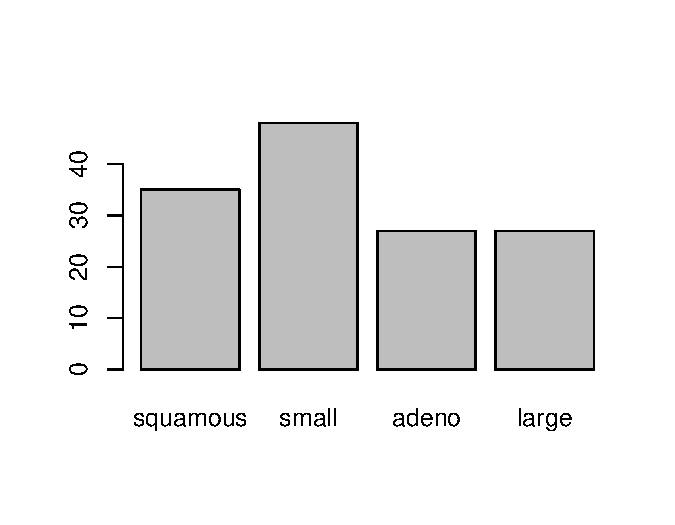
\includegraphics{R_BioST_book_files/figure-latex/unnamed-chunk-45-1.pdf}

\begin{verbatim}
##      [,1]
## [1,]  0.7
## [2,]  1.9
## [3,]  3.1
## [4,]  4.3
pie(cellcode.tab)
\end{verbatim}

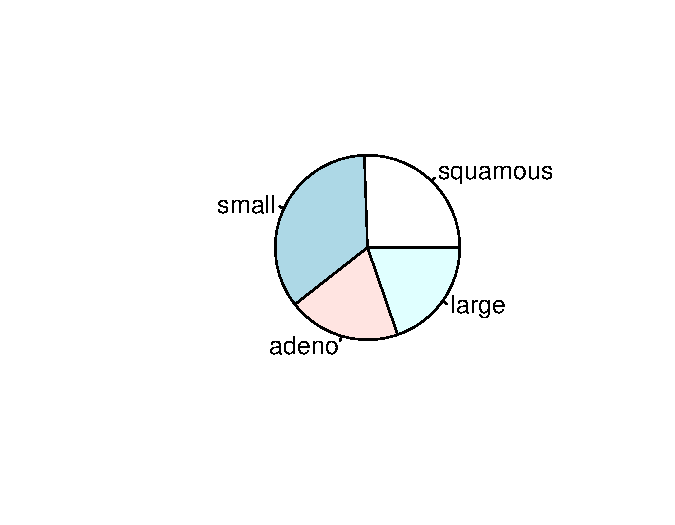
\includegraphics{R_BioST_book_files/figure-latex/unnamed-chunk-45-2.pdf}

\begin{Shaded}
\begin{Highlighting}[]
\KeywordTok{library}\NormalTok{(ggplot2)}
\CommentTok{\#\# bar chart}
\KeywordTok{ggplot}\NormalTok{(}\DataTypeTok{data =}\NormalTok{ dd, }\KeywordTok{aes}\NormalTok{(}\DataTypeTok{x =}\NormalTok{ cellcode)) }\OperatorTok{+}
\StringTok{  }\KeywordTok{geom\_bar}\NormalTok{(}\DataTypeTok{treat =} \StringTok{"blue"}\NormalTok{)}
\CommentTok{\#\# Warning: Ignoring unknown parameters: treat}
\end{Highlighting}
\end{Shaded}

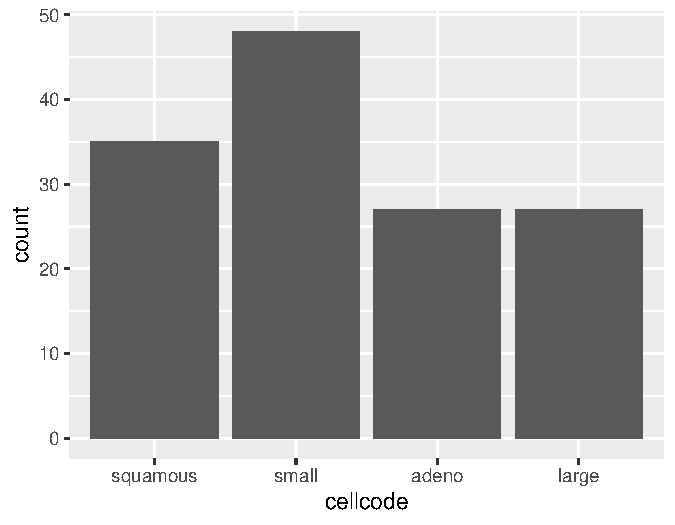
\includegraphics{R_BioST_book_files/figure-latex/unnamed-chunk-45-3.pdf}

\begin{Shaded}
\begin{Highlighting}[]
\KeywordTok{ggplot}\NormalTok{(}\DataTypeTok{data =}\NormalTok{ dd, }\KeywordTok{aes}\NormalTok{(}\DataTypeTok{x =}\NormalTok{ cellcode)) }\OperatorTok{+}
\StringTok{  }\KeywordTok{geom\_bar}\NormalTok{(}\DataTypeTok{treat =} \StringTok{"blue"}\NormalTok{) }\OperatorTok{+}\StringTok{ }
\StringTok{  }\KeywordTok{coord\_flip}\NormalTok{()}
\CommentTok{\#\# Warning: Ignoring unknown parameters: treat}
\end{Highlighting}
\end{Shaded}

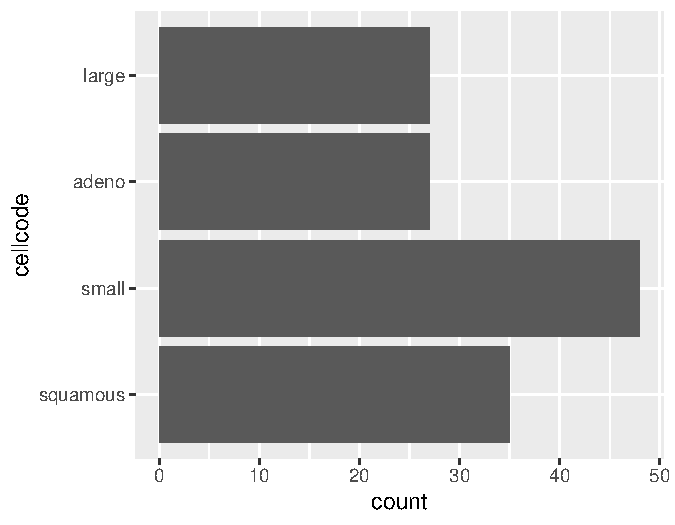
\includegraphics{R_BioST_book_files/figure-latex/unnamed-chunk-45-4.pdf}

\begin{Shaded}
\begin{Highlighting}[]
\KeywordTok{ggplot}\NormalTok{(}\DataTypeTok{data =}\NormalTok{ dd, }\KeywordTok{aes}\NormalTok{(}\DataTypeTok{y =}\NormalTok{ cellcode)) }\OperatorTok{+}
\StringTok{  }\KeywordTok{geom\_bar}\NormalTok{(}\DataTypeTok{treat =} \StringTok{"blue"}\NormalTok{) }
\CommentTok{\#\# Warning: Ignoring unknown parameters: treat}
\end{Highlighting}
\end{Shaded}

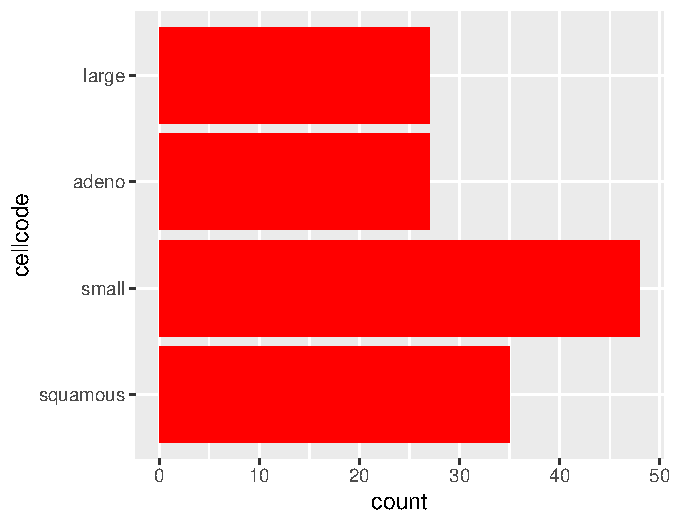
\includegraphics{R_BioST_book_files/figure-latex/unnamed-chunk-45-5.pdf}

\begin{Shaded}
\begin{Highlighting}[]
\CommentTok{\# pie chart: no simple solution}
\NormalTok{clar.freq \textless{}{-}}\StringTok{ }\KeywordTok{data.frame}\NormalTok{(cellcode.tab)}
\KeywordTok{names}\NormalTok{(clar.freq)[}\DecValTok{1}\NormalTok{] \textless{}{-}}\StringTok{ "cellcode"}
\NormalTok{clar.freq}
\CommentTok{\#\#   cellcode Freq}
\CommentTok{\#\# 1 squamous   35}
\CommentTok{\#\# 2    small   48}
\CommentTok{\#\# 3    adeno   27}
\CommentTok{\#\# 4    large   27}
\KeywordTok{ggplot}\NormalTok{(}\DataTypeTok{data =}\NormalTok{ clar.freq, }\KeywordTok{aes}\NormalTok{(}\DataTypeTok{x =} \StringTok{""}\NormalTok{, }\DataTypeTok{y =}\NormalTok{ Freq, }\DataTypeTok{fill =}\NormalTok{ cellcode)) }\OperatorTok{+}
\StringTok{  }\KeywordTok{geom\_bar}\NormalTok{(}\DataTypeTok{width =} \DecValTok{1}\NormalTok{, }\DataTypeTok{stat =} \StringTok{"identity"}\NormalTok{) }\OperatorTok{+}\StringTok{ }
\StringTok{  }\KeywordTok{coord\_polar}\NormalTok{(}\StringTok{"y"}\NormalTok{, }\DataTypeTok{start =} \DecValTok{0}\NormalTok{)}
\end{Highlighting}
\end{Shaded}

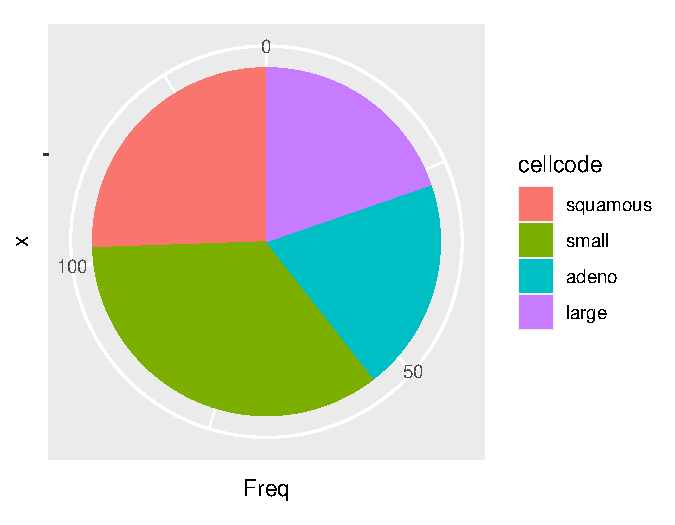
\includegraphics{R_BioST_book_files/figure-latex/unnamed-chunk-45-6.pdf}

\begin{Shaded}
\begin{Highlighting}[]
\KeywordTok{ggplot}\NormalTok{(}\DataTypeTok{data =}\NormalTok{ clar.freq, }\KeywordTok{aes}\NormalTok{(}\DataTypeTok{x =} \StringTok{""}\NormalTok{, }\DataTypeTok{y =}\NormalTok{ Freq, }\DataTypeTok{fill =}\NormalTok{ cellcode)) }\OperatorTok{+}
\StringTok{  }\KeywordTok{geom\_bar}\NormalTok{(}\DataTypeTok{stat =} \StringTok{"identity"}\NormalTok{, }\DataTypeTok{width =} \DecValTok{1}\NormalTok{, }\DataTypeTok{treat =} \StringTok{"white"}\NormalTok{) }\OperatorTok{+}
\StringTok{  }\KeywordTok{coord\_polar}\NormalTok{(}\DataTypeTok{theta =} \StringTok{"y"}\NormalTok{, }\DataTypeTok{start =} \DecValTok{0}\NormalTok{) }\OperatorTok{+}
\StringTok{  }\KeywordTok{theme\_void}\NormalTok{() }\CommentTok{\# remove background}
\CommentTok{\#\# Warning: Ignoring unknown parameters: treat}
\end{Highlighting}
\end{Shaded}

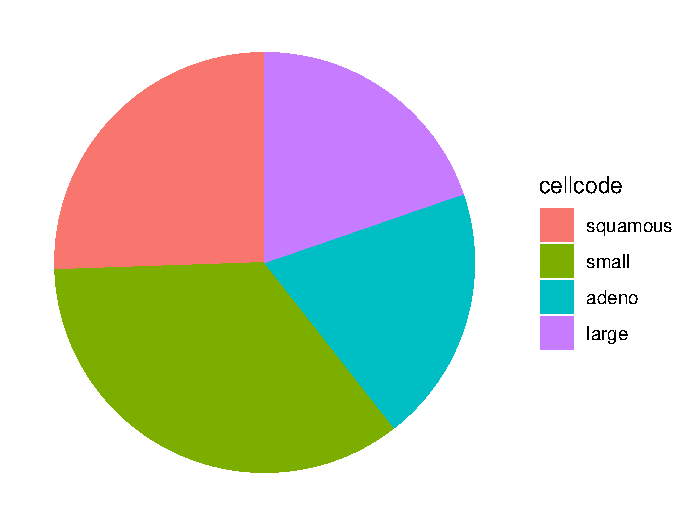
\includegraphics{R_BioST_book_files/figure-latex/unnamed-chunk-45-7.pdf}

\hypertarget{ux591aux985eux5225ux8b8aux6578}{%
\subsection{多類別變數}\label{ux591aux985eux5225ux8b8aux6578}}

\begin{itemize}
\tightlist
\item
  雙類別變數: 檢視變數聯合水準的頻率大小,
  檢視條件水準的頻率大小.
\end{itemize}

\begin{Shaded}
\begin{Highlighting}[]
\CommentTok{\#\# two categorical vtriables}
\KeywordTok{table}\NormalTok{(dd}\OperatorTok{$}\NormalTok{treat)}
\CommentTok{\#\# }
\CommentTok{\#\# placebo    test }
\CommentTok{\#\#      69      68}
\KeywordTok{table}\NormalTok{(dd}\OperatorTok{$}\NormalTok{cellcode)}
\CommentTok{\#\# }
\CommentTok{\#\# squamous    small    adeno    large }
\CommentTok{\#\#       35       48       27       27}
\NormalTok{twoway.tab \textless{}{-}}\StringTok{ }\KeywordTok{table}\NormalTok{(dd}\OperatorTok{$}\NormalTok{treat, dd}\OperatorTok{$}\NormalTok{cellcode)}
\NormalTok{twoway.tab}
\CommentTok{\#\#          }
\CommentTok{\#\#           squamous small adeno large}
\CommentTok{\#\#   placebo       15    30     9    15}
\CommentTok{\#\#   test          20    18    18    12}
\CommentTok{\#\# \# cell proportion}
\NormalTok{cell.prop \textless{}{-}}\StringTok{ }\KeywordTok{prop.table}\NormalTok{(twoway.tab, }\DataTypeTok{margin=}\OtherTok{NULL}\NormalTok{) }
\KeywordTok{round}\NormalTok{(cell.prop, }\DecValTok{3}\NormalTok{)}
\CommentTok{\#\#          }
\CommentTok{\#\#           squamous small adeno large}
\CommentTok{\#\#   placebo    0.109 0.219 0.066 0.109}
\CommentTok{\#\#   test       0.146 0.131 0.131 0.088}
\CommentTok{\#\# conditional on row sum to 1}
\NormalTok{cond\_row\_prop \textless{}{-}}\StringTok{ }\KeywordTok{prop.table}\NormalTok{(twoway.tab, }\DataTypeTok{margin =} \DecValTok{1}\NormalTok{) }
\KeywordTok{round}\NormalTok{(cond\_row\_prop, }\DecValTok{3}\NormalTok{)}
\CommentTok{\#\#          }
\CommentTok{\#\#           squamous small adeno large}
\CommentTok{\#\#   placebo    0.217 0.435 0.130 0.217}
\CommentTok{\#\#   test       0.294 0.265 0.265 0.176}
\KeywordTok{apply}\NormalTok{(cond\_row\_prop, }\DecValTok{1}\NormalTok{, sum) }\CommentTok{\# rows sum to 1}
\CommentTok{\#\# placebo    test }
\CommentTok{\#\#       1       1}
\CommentTok{\#\# conditional on column sum to 1}
\NormalTok{cond\_col\_prop \textless{}{-}}\StringTok{ }\KeywordTok{prop.table}\NormalTok{(twoway.tab, }\DataTypeTok{margin =} \DecValTok{2}\NormalTok{) }
\KeywordTok{round}\NormalTok{(cond\_col\_prop, }\DecValTok{3}\NormalTok{)}
\CommentTok{\#\#          }
\CommentTok{\#\#           squamous small adeno large}
\CommentTok{\#\#   placebo    0.429 0.625 0.333 0.556}
\CommentTok{\#\#   test       0.571 0.375 0.667 0.444}
\KeywordTok{apply}\NormalTok{(cond\_col\_prop, }\DecValTok{2}\NormalTok{, sum) }\CommentTok{\# cols sum to 1}
\CommentTok{\#\# squamous    small    adeno    large }
\CommentTok{\#\#        1        1        1        1}
\CommentTok{\#\# side{-}by{-}side bar plot}
\KeywordTok{barplot}\NormalTok{(twoway.tab, }
        \DataTypeTok{beside =} \OtherTok{TRUE}\NormalTok{, }
        \DataTypeTok{main =} \StringTok{"treat By cellcode"}\NormalTok{,}
        \DataTypeTok{xlab =} \StringTok{"clarty"}\NormalTok{)}
\end{Highlighting}
\end{Shaded}

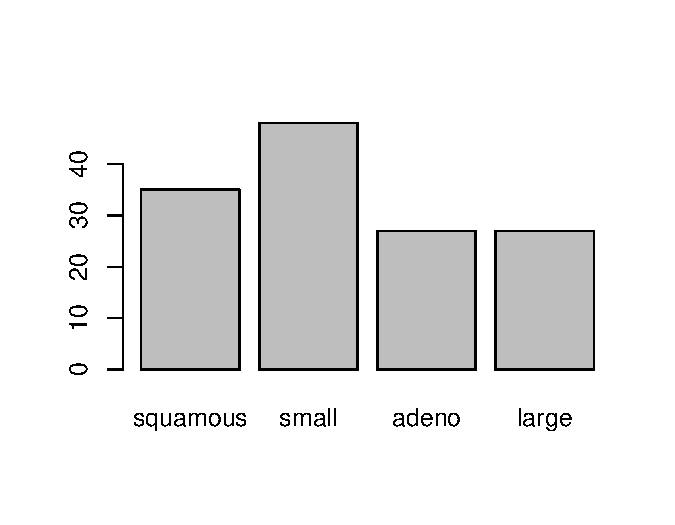
\includegraphics{R_BioST_book_files/figure-latex/unnamed-chunk-46-1.pdf}

\begin{Shaded}
\begin{Highlighting}[]
\CommentTok{\# Stacked Bar Plot}
\KeywordTok{barplot}\NormalTok{(twoway.tab,}
        \DataTypeTok{beside =} \OtherTok{FALSE}\NormalTok{, }
        \DataTypeTok{main =} \StringTok{"treat By cellcode"}\NormalTok{,}
        \DataTypeTok{xlab =} \StringTok{"treat"}\NormalTok{)}
\end{Highlighting}
\end{Shaded}

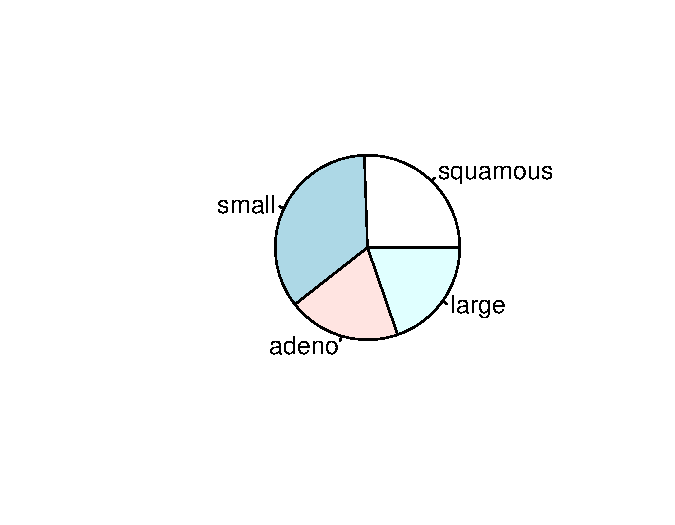
\includegraphics{R_BioST_book_files/figure-latex/unnamed-chunk-46-2.pdf}

\begin{Shaded}
\begin{Highlighting}[]
\CommentTok{\#\# ggplot2}
\CommentTok{\#\# Automatically stack}
\KeywordTok{library}\NormalTok{(ggplot2)}
\KeywordTok{ggplot}\NormalTok{(}\DataTypeTok{data =}\NormalTok{ dd, }\KeywordTok{aes}\NormalTok{(}\DataTypeTok{x =}\NormalTok{ cellcode, }\DataTypeTok{fill =}\NormalTok{ treat)) }\OperatorTok{+}\StringTok{ }
\StringTok{  }\KeywordTok{geom\_bar}\NormalTok{()}
\end{Highlighting}
\end{Shaded}

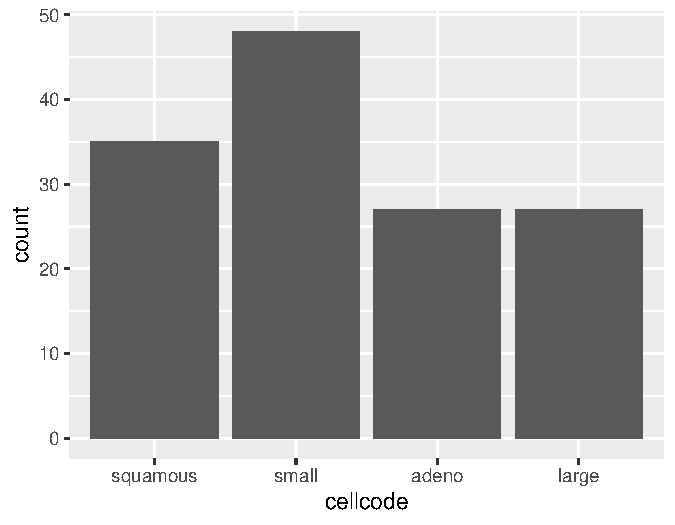
\includegraphics{R_BioST_book_files/figure-latex/unnamed-chunk-46-3.pdf}

\begin{Shaded}
\begin{Highlighting}[]
\KeywordTok{ggplot}\NormalTok{(}\DataTypeTok{data =}\NormalTok{ dd, }\KeywordTok{aes}\NormalTok{(}\DataTypeTok{x =}\NormalTok{ cellcode, }\DataTypeTok{fill =}\NormalTok{ treat)) }\OperatorTok{+}
\StringTok{  }\KeywordTok{geom\_bar}\NormalTok{(}\DataTypeTok{position =} \StringTok{"stack"}\NormalTok{)}
\end{Highlighting}
\end{Shaded}

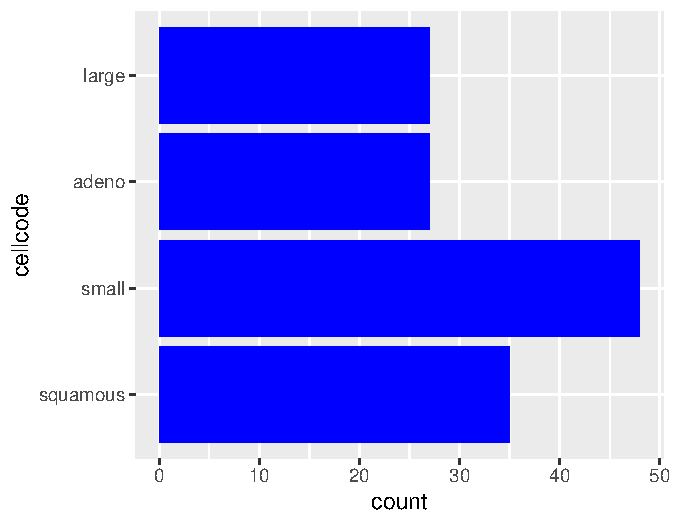
\includegraphics{R_BioST_book_files/figure-latex/unnamed-chunk-46-4.pdf}

\begin{Shaded}
\begin{Highlighting}[]
\CommentTok{\#\# side{-}by{-}side }
\KeywordTok{ggplot}\NormalTok{(}\DataTypeTok{data =}\NormalTok{ dd, }\KeywordTok{aes}\NormalTok{(}\DataTypeTok{x =}\NormalTok{ cellcode, }\DataTypeTok{fill =}\NormalTok{ treat)) }\OperatorTok{+}\StringTok{ }
\StringTok{  }\KeywordTok{geom\_bar}\NormalTok{(}\DataTypeTok{position =} \StringTok{"dodge"}\NormalTok{)}
\end{Highlighting}
\end{Shaded}

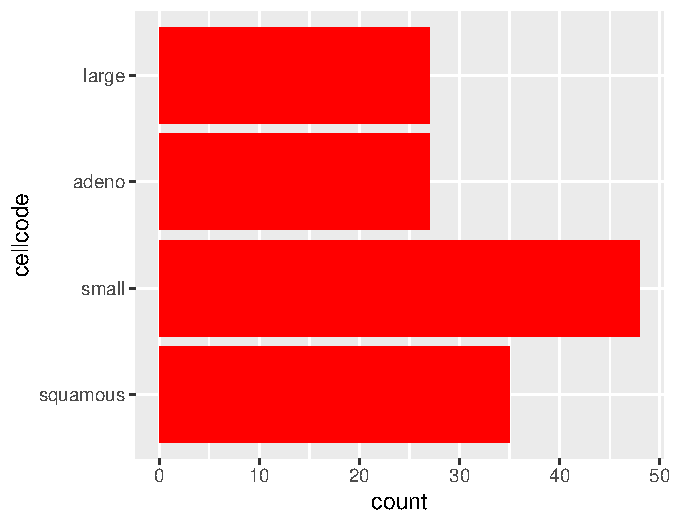
\includegraphics{R_BioST_book_files/figure-latex/unnamed-chunk-46-5.pdf}

\begin{Shaded}
\begin{Highlighting}[]
\KeywordTok{ggplot}\NormalTok{(}\DataTypeTok{data =}\NormalTok{ dd, }\KeywordTok{aes}\NormalTok{(}\DataTypeTok{x =}\NormalTok{ cellcode, }\DataTypeTok{fill =}\NormalTok{ treat)) }\OperatorTok{+}\StringTok{ }
\StringTok{  }\KeywordTok{geom\_bar}\NormalTok{(}\DataTypeTok{position =} \StringTok{"fill"}\NormalTok{)}
\end{Highlighting}
\end{Shaded}

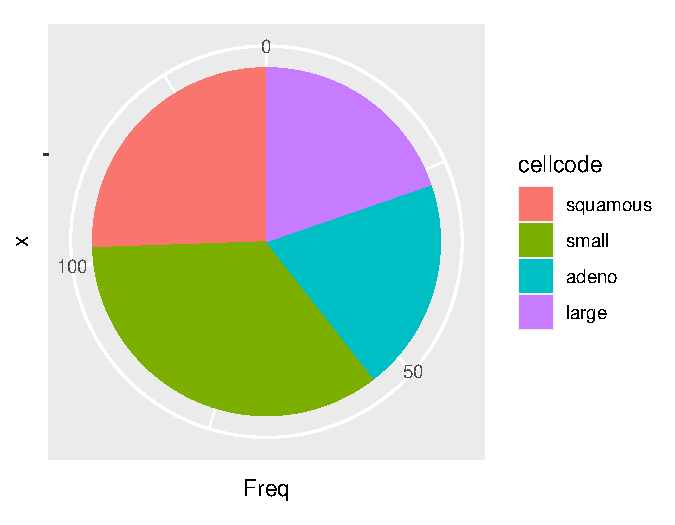
\includegraphics{R_BioST_book_files/figure-latex/unnamed-chunk-46-6.pdf}

\hypertarget{ux9023ux7e8cux8b8aux6578}{%
\section{連續變數}\label{ux9023ux7e8cux8b8aux6578}}

連續變數描述性統計主要是分析變數的
\textbf{分配}
或
\textbf{分佈}
(\textbf{distribution}),
分配敘述變數的觀測數值以及這些觀測數值出現的頻率.
連續變數描述性統計圖表常見為
點狀圖 (dot plot), 枝葉圖 (stem-and-leaf),
次數分配表, 直方圖 (histogram), 盒鬚圖 (box plot),
密度圖 (density plot), 平均值, 變異數等.
對連續變數的描述, 若樣本數較少,
常使用點狀圖或枝葉圖.
目前多數為大數據, 點狀圖或枝葉圖較少使用,
但在實驗設計的數據呈現仍然非常重要.

\hypertarget{ux55aeux9023ux7e8cux8b8aux6578}{%
\subsection{單連續變數}\label{ux55aeux9023ux7e8cux8b8aux6578}}

\begin{itemize}
\tightlist
\item
  單連續變數: 檢視中央趨勢, 離散程度 偏度, 峰度.
\end{itemize}

\begin{Shaded}
\begin{Highlighting}[]
\CommentTok{\#\# use R base pie()}
\CommentTok{\#\# histogram}
\KeywordTok{hist}\NormalTok{(dd}\OperatorTok{$}\NormalTok{time, }
     \DataTypeTok{freq =} \OtherTok{TRUE}\NormalTok{,    }
     \DataTypeTok{main =} \StringTok{"time histogram"}\NormalTok{,}
     \DataTypeTok{xlab =} \StringTok{"time"}\NormalTok{)}
\end{Highlighting}
\end{Shaded}

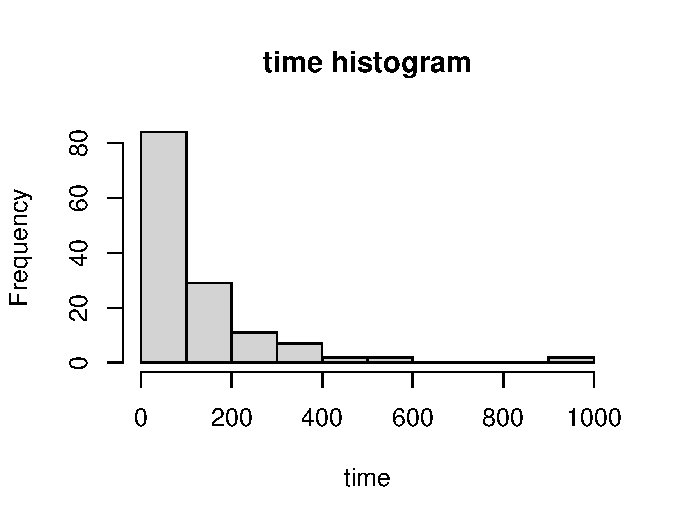
\includegraphics{R_BioST_book_files/figure-latex/unnamed-chunk-47-1.pdf}

\begin{Shaded}
\begin{Highlighting}[]
\KeywordTok{hist}\NormalTok{(dd}\OperatorTok{$}\NormalTok{time, }
     \DataTypeTok{freq =} \OtherTok{FALSE}\NormalTok{,    }
     \DataTypeTok{main =} \StringTok{"time histogram"}\NormalTok{,}
     \DataTypeTok{xlab =} \StringTok{"time"}\NormalTok{)}
\end{Highlighting}
\end{Shaded}

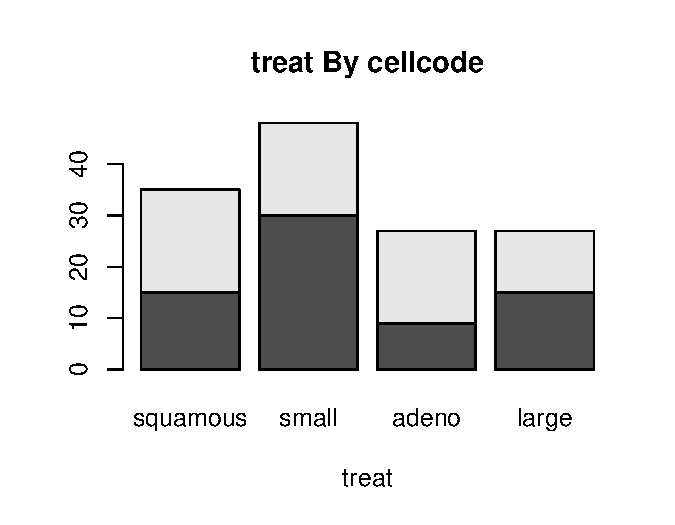
\includegraphics{R_BioST_book_files/figure-latex/unnamed-chunk-47-2.pdf}

\begin{Shaded}
\begin{Highlighting}[]
\CommentTok{\# box plot}
\KeywordTok{boxplot}\NormalTok{(dd}\OperatorTok{$}\NormalTok{time, }
        \DataTypeTok{xlab =} \StringTok{"time"}\NormalTok{)}
\end{Highlighting}
\end{Shaded}

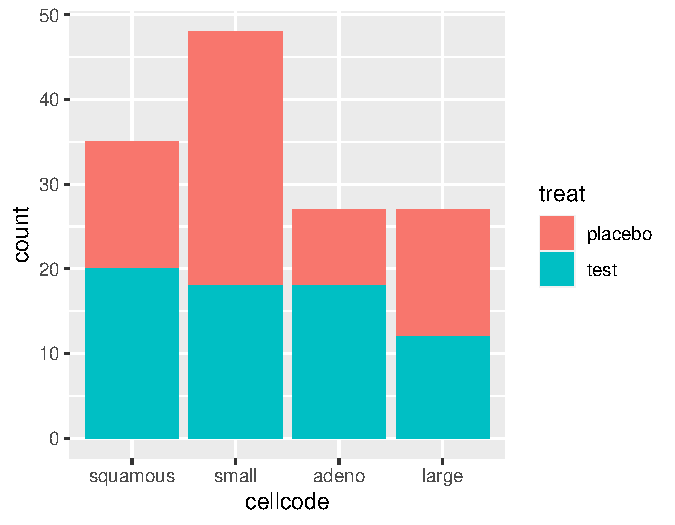
\includegraphics{R_BioST_book_files/figure-latex/unnamed-chunk-47-3.pdf}

\begin{Shaded}
\begin{Highlighting}[]
\CommentTok{\# QQ plot}
\KeywordTok{qqnorm}\NormalTok{(dd}\OperatorTok{$}\NormalTok{time, }
       \DataTypeTok{main =} \StringTok{"Normal QQ Plot: time"}\NormalTok{)}
\end{Highlighting}
\end{Shaded}

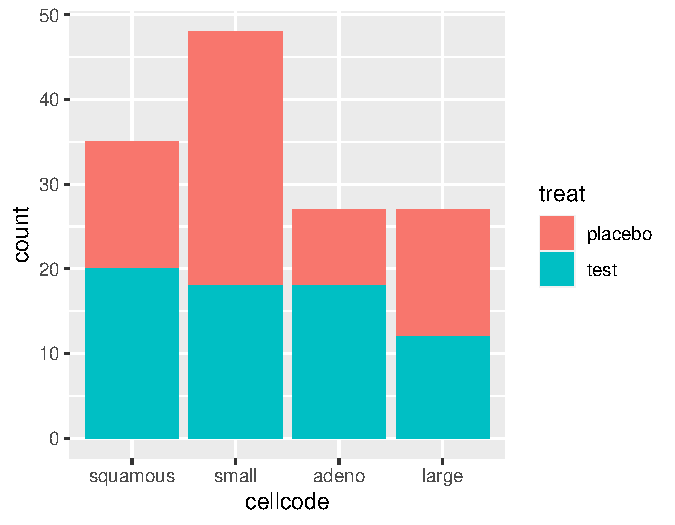
\includegraphics{R_BioST_book_files/figure-latex/unnamed-chunk-47-4.pdf}

\begin{Shaded}
\begin{Highlighting}[]
\CommentTok{\# density plot}
\KeywordTok{plot}\NormalTok{(}\KeywordTok{density}\NormalTok{(dd}\OperatorTok{$}\NormalTok{time),}
     \DataTypeTok{pch =} \DecValTok{16}\NormalTok{,}
     \DataTypeTok{main =} \StringTok{"Density Plot"}\NormalTok{,}
     \DataTypeTok{xlab =} \StringTok{"time"}\NormalTok{,}
     \DataTypeTok{ylab =} \StringTok{"density"}\NormalTok{)}
\end{Highlighting}
\end{Shaded}

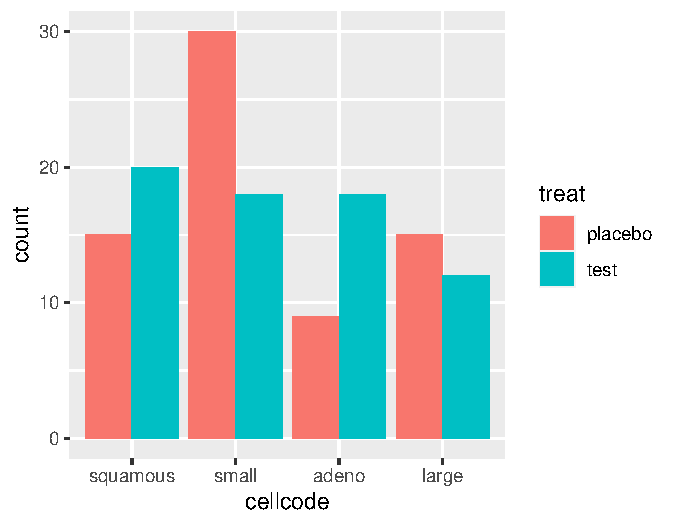
\includegraphics{R_BioST_book_files/figure-latex/unnamed-chunk-47-5.pdf}

\begin{Shaded}
\begin{Highlighting}[]
\CommentTok{\#\# ggplot2 }
\CommentTok{\#\# histogram}
\KeywordTok{ggplot}\NormalTok{(}\DataTypeTok{data =}\NormalTok{ dd, }\KeywordTok{aes}\NormalTok{(}\DataTypeTok{x =}\NormalTok{ time)) }\OperatorTok{+}\StringTok{ }
\StringTok{  }\KeywordTok{geom\_histogram}\NormalTok{()}
\end{Highlighting}
\end{Shaded}

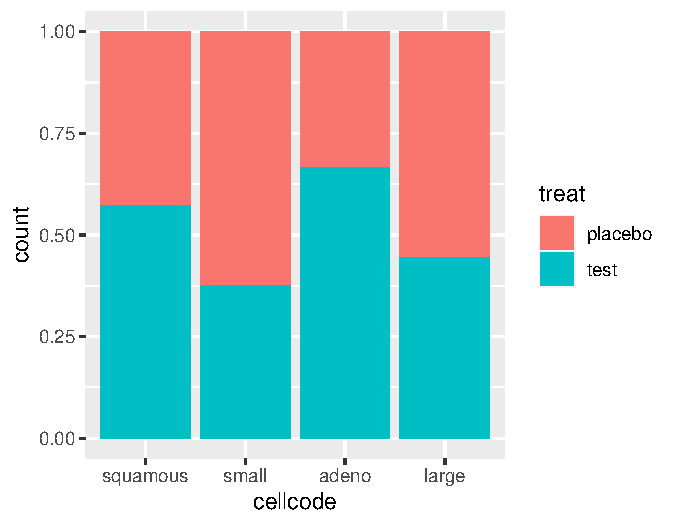
\includegraphics{R_BioST_book_files/figure-latex/unnamed-chunk-47-6.pdf}

\begin{Shaded}
\begin{Highlighting}[]
\CommentTok{\#\# box plot}
\KeywordTok{ggplot}\NormalTok{(dd, }\KeywordTok{aes}\NormalTok{(}\DataTypeTok{x =} \StringTok{""}\NormalTok{, }\DataTypeTok{y =}\NormalTok{ time)) }\OperatorTok{+}\StringTok{ }
\StringTok{  }\KeywordTok{geom\_boxplot}\NormalTok{()}
\end{Highlighting}
\end{Shaded}

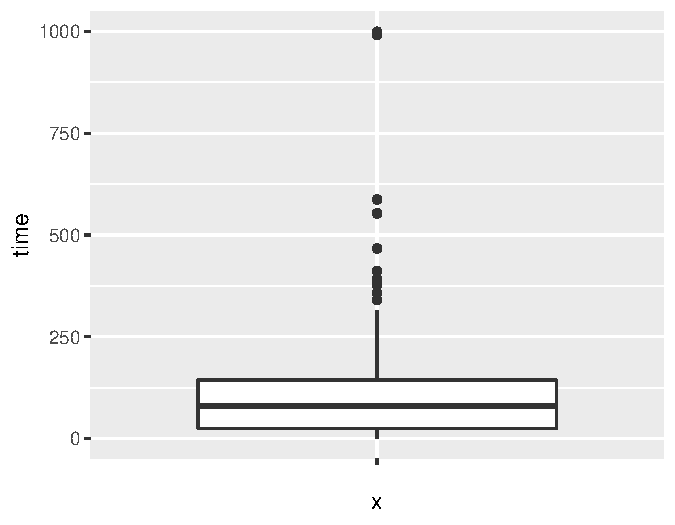
\includegraphics{R_BioST_book_files/figure-latex/unnamed-chunk-47-7.pdf}

\begin{Shaded}
\begin{Highlighting}[]
\CommentTok{\#\# violin plot}
\KeywordTok{ggplot}\NormalTok{(dd, }\KeywordTok{aes}\NormalTok{(}\DataTypeTok{x =} \StringTok{""}\NormalTok{, }\DataTypeTok{y =}\NormalTok{ time)) }\OperatorTok{+}\StringTok{ }
\StringTok{  }\KeywordTok{geom\_violin}\NormalTok{()}
\end{Highlighting}
\end{Shaded}

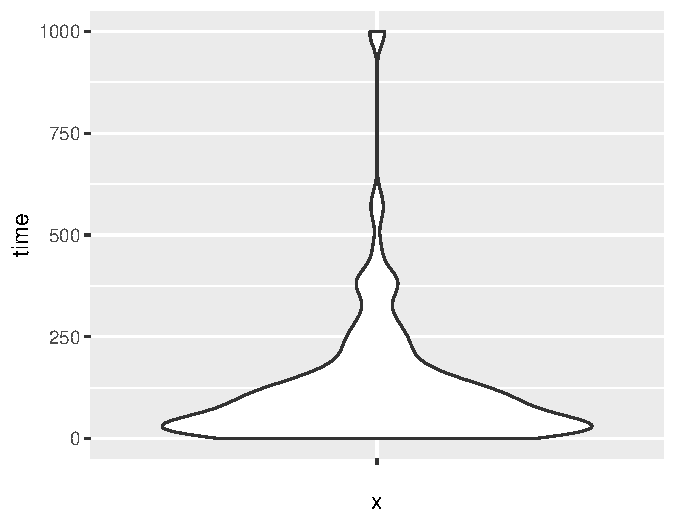
\includegraphics{R_BioST_book_files/figure-latex/unnamed-chunk-47-8.pdf}

\begin{Shaded}
\begin{Highlighting}[]
\CommentTok{\#\# density plot}
\KeywordTok{ggplot}\NormalTok{(}\DataTypeTok{data =}\NormalTok{ dd, }\KeywordTok{aes}\NormalTok{(}\DataTypeTok{x =}\NormalTok{ time)) }\OperatorTok{+}\StringTok{ }
\StringTok{  }\KeywordTok{geom\_freqpoly}\NormalTok{()}
\end{Highlighting}
\end{Shaded}

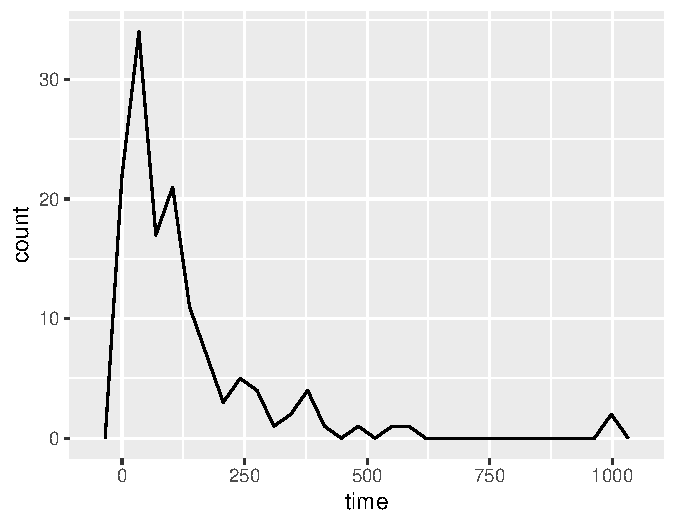
\includegraphics{R_BioST_book_files/figure-latex/unnamed-chunk-47-9.pdf}

\begin{Shaded}
\begin{Highlighting}[]
\KeywordTok{ggplot}\NormalTok{(}\DataTypeTok{data =}\NormalTok{ dd, }\KeywordTok{aes}\NormalTok{(}\DataTypeTok{x =}\NormalTok{ time)) }\OperatorTok{+}\StringTok{ }
\StringTok{  }\KeywordTok{stat\_bin}\NormalTok{(}\DataTypeTok{geom =} \StringTok{"area"}\NormalTok{)}
\end{Highlighting}
\end{Shaded}

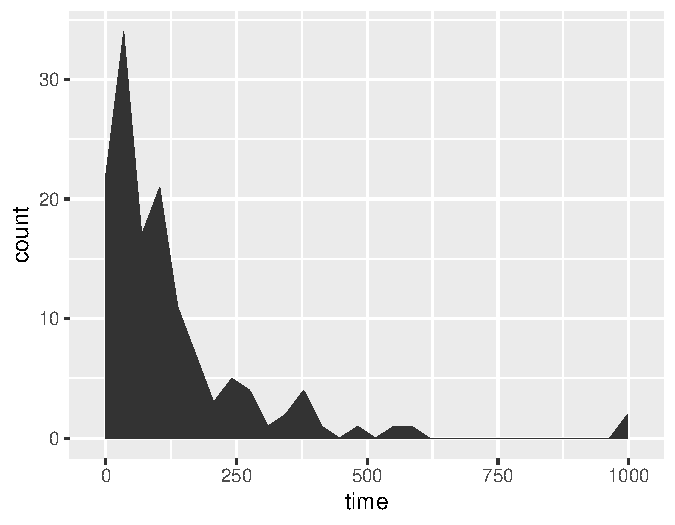
\includegraphics{R_BioST_book_files/figure-latex/unnamed-chunk-47-10.pdf}

\begin{Shaded}
\begin{Highlighting}[]
\KeywordTok{ggplot}\NormalTok{(}\DataTypeTok{data =}\NormalTok{ dd, }\KeywordTok{aes}\NormalTok{(}\DataTypeTok{x =}\NormalTok{ time)) }\OperatorTok{+}\StringTok{ }
\StringTok{  }\KeywordTok{stat\_bin}\NormalTok{(}\DataTypeTok{geom =} \StringTok{"line"}\NormalTok{)}
\end{Highlighting}
\end{Shaded}

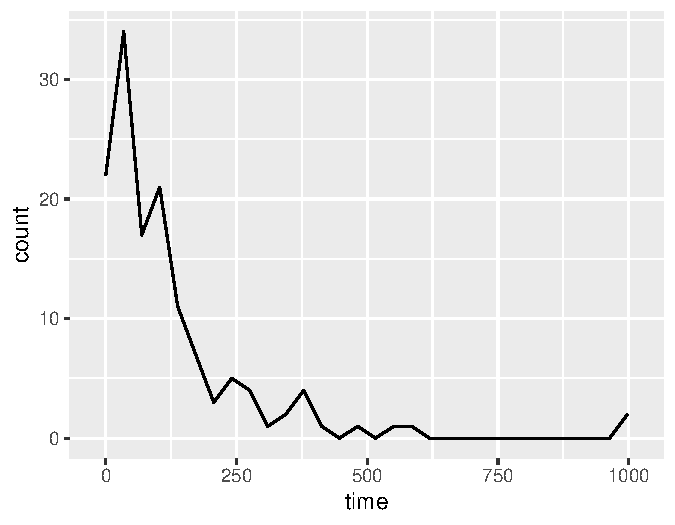
\includegraphics{R_BioST_book_files/figure-latex/unnamed-chunk-47-11.pdf}

\hypertarget{ux4e8cux9023ux7e8cux8b8aux6578}{%
\subsection{二連續變數}\label{ux4e8cux9023ux7e8cux8b8aux6578}}

\begin{itemize}
\tightlist
\item
  散佈圖 \textbf{scatter plot} = X \& Y = 連續變數
\item
  雙連續變數: 檢視二個變數關聯性, 大小, 方向, 趨勢.
\end{itemize}

\begin{Shaded}
\begin{Highlighting}[]
\CommentTok{\#\# R base}
\CommentTok{\#\# scatter plot}
\CommentTok{\#\# basic}
\KeywordTok{plot}\NormalTok{(}\DataTypeTok{x =}\NormalTok{ dd}\OperatorTok{$}\NormalTok{diagtime, }\DataTypeTok{y =}\NormalTok{ dd}\OperatorTok{$}\NormalTok{time)}
\end{Highlighting}
\end{Shaded}

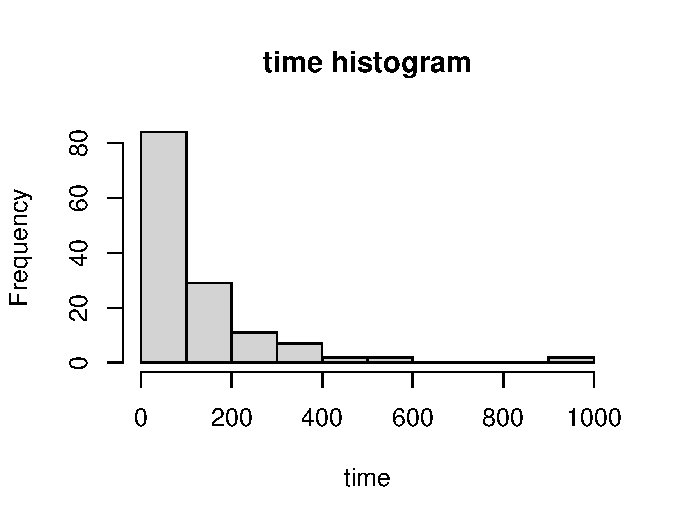
\includegraphics{R_BioST_book_files/figure-latex/unnamed-chunk-48-1.pdf}

\begin{Shaded}
\begin{Highlighting}[]
\CommentTok{\#\# formulat y \textasciitilde{} x, data = data\_name)}
\KeywordTok{plot}\NormalTok{(time }\OperatorTok{\textasciitilde{}}\StringTok{ }\NormalTok{diagtime, }\DataTypeTok{data =}\NormalTok{ dd)}
\end{Highlighting}
\end{Shaded}

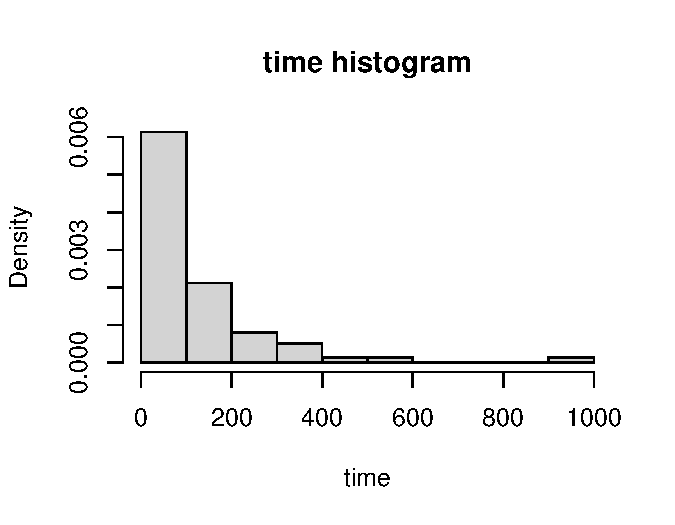
\includegraphics{R_BioST_book_files/figure-latex/unnamed-chunk-48-2.pdf}

\begin{Shaded}
\begin{Highlighting}[]
\CommentTok{\#\# ggplot}
\KeywordTok{ggplot}\NormalTok{(}\DataTypeTok{data =}\NormalTok{ dd, }\KeywordTok{aes}\NormalTok{(}\DataTypeTok{x =}\NormalTok{ diagtime, }\DataTypeTok{y =}\NormalTok{ time)) }\OperatorTok{+}\StringTok{ }
\StringTok{  }\KeywordTok{geom\_point}\NormalTok{()}
\end{Highlighting}
\end{Shaded}

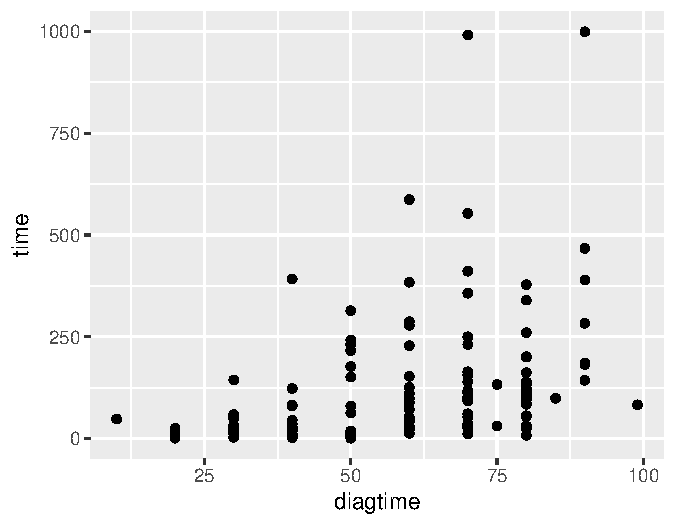
\includegraphics{R_BioST_book_files/figure-latex/unnamed-chunk-48-3.pdf}

\begin{Shaded}
\begin{Highlighting}[]
\KeywordTok{ggplot}\NormalTok{(}\DataTypeTok{data =}\NormalTok{ dd, }\KeywordTok{aes}\NormalTok{(}\DataTypeTok{x =}\NormalTok{ diagtime, }\DataTypeTok{y =}\NormalTok{ time)) }\OperatorTok{+}\StringTok{ }
\StringTok{  }\KeywordTok{geom\_point}\NormalTok{(}\DataTypeTok{size =} \DecValTok{5}\NormalTok{)}
\end{Highlighting}
\end{Shaded}

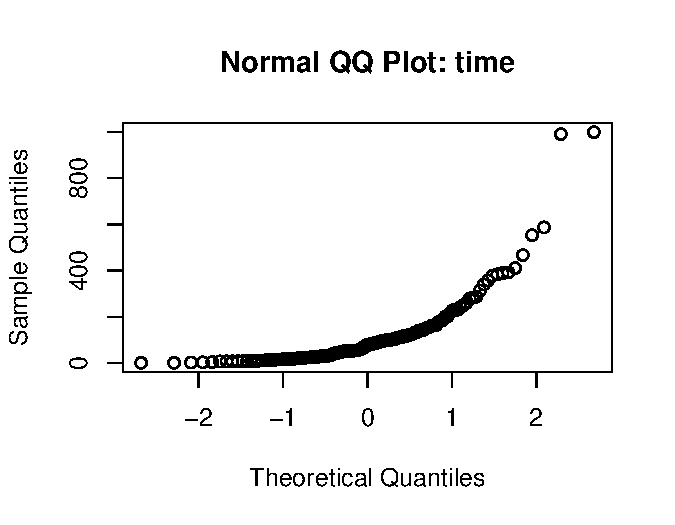
\includegraphics{R_BioST_book_files/figure-latex/unnamed-chunk-48-4.pdf}

\begin{Shaded}
\begin{Highlighting}[]
\KeywordTok{ggplot}\NormalTok{(}\DataTypeTok{data =}\NormalTok{ dd, }\KeywordTok{aes}\NormalTok{(}\DataTypeTok{x =}\NormalTok{ diagtime, }\DataTypeTok{y =}\NormalTok{ time)) }\OperatorTok{+}\StringTok{ }
\StringTok{  }\KeywordTok{geom\_jitter}\NormalTok{() }
\end{Highlighting}
\end{Shaded}

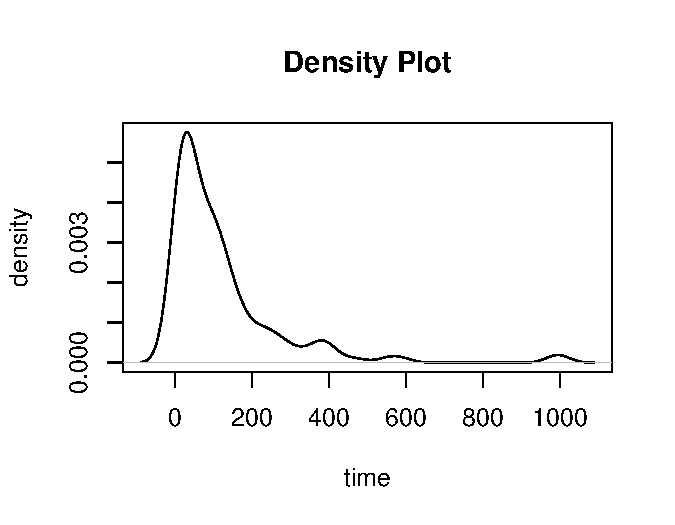
\includegraphics{R_BioST_book_files/figure-latex/unnamed-chunk-48-5.pdf}

\begin{Shaded}
\begin{Highlighting}[]
\KeywordTok{ggplot}\NormalTok{(}\DataTypeTok{data =}\NormalTok{ dd, }\KeywordTok{aes}\NormalTok{(}\DataTypeTok{x =}\NormalTok{ diagtime, }\DataTypeTok{y =}\NormalTok{ time)) }\OperatorTok{+}\StringTok{ }
\StringTok{  }\KeywordTok{geom\_jitter}\NormalTok{(}\DataTypeTok{size =} \DecValTok{5}\NormalTok{, }\DataTypeTok{alpha =} \DecValTok{1}\OperatorTok{/}\DecValTok{2}\NormalTok{) }
\end{Highlighting}
\end{Shaded}

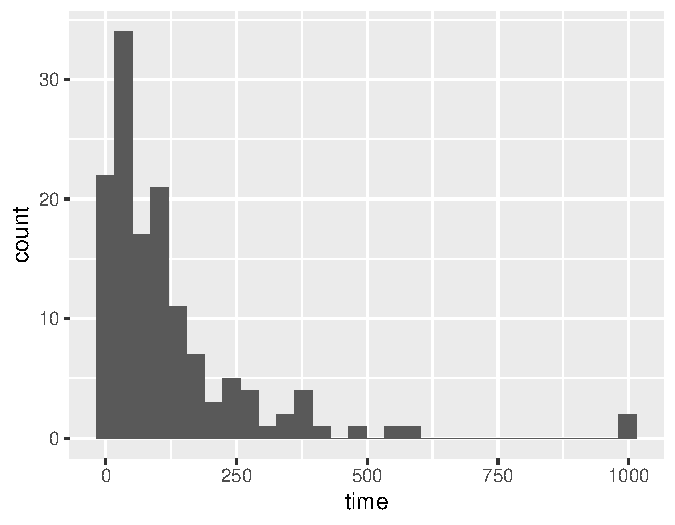
\includegraphics{R_BioST_book_files/figure-latex/unnamed-chunk-48-6.pdf}

\begin{Shaded}
\begin{Highlighting}[]
\KeywordTok{ggplot}\NormalTok{(}\DataTypeTok{data =}\NormalTok{ dd, }\KeywordTok{aes}\NormalTok{(}\DataTypeTok{x =}\NormalTok{ diagtime, }\DataTypeTok{y =}\NormalTok{ time)) }\OperatorTok{+}\StringTok{ }
\StringTok{  }\KeywordTok{geom\_jitter}\NormalTok{(}\DataTypeTok{size =} \DecValTok{5}\NormalTok{, }\DataTypeTok{alpha =} \FloatTok{0.3}\NormalTok{) }\OperatorTok{+}\StringTok{ }
\StringTok{  }\KeywordTok{geom\_rug}\NormalTok{(}\DataTypeTok{col =} \StringTok{"steelblue"}\NormalTok{, }\DataTypeTok{alpha =} \FloatTok{0.1}\NormalTok{, }\DataTypeTok{size =} \FloatTok{1.5}\NormalTok{)}
\end{Highlighting}
\end{Shaded}

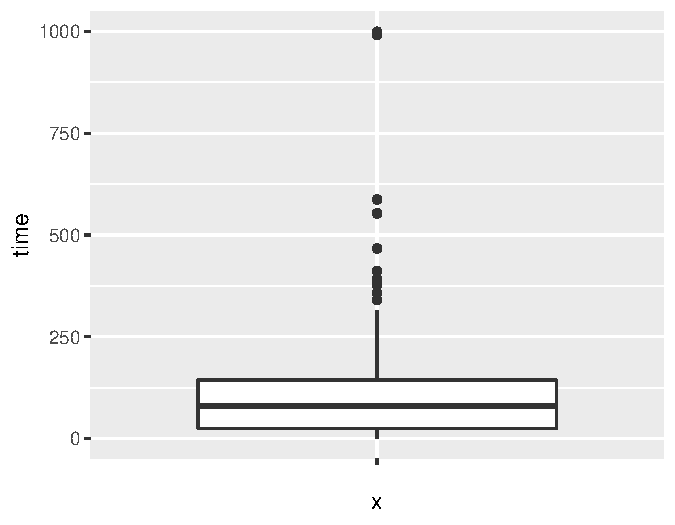
\includegraphics{R_BioST_book_files/figure-latex/unnamed-chunk-48-7.pdf}

\begin{Shaded}
\begin{Highlighting}[]
\CommentTok{\# add linear line or smoothing line}
\KeywordTok{ggplot}\NormalTok{(}\DataTypeTok{data =}\NormalTok{ dd, }\KeywordTok{aes}\NormalTok{(}\DataTypeTok{x =}\NormalTok{ diagtime, }\DataTypeTok{y =}\NormalTok{ time)) }\OperatorTok{+}\StringTok{ }
\StringTok{  }\KeywordTok{geom\_point}\NormalTok{() }\OperatorTok{+}\StringTok{ }
\StringTok{  }\KeywordTok{geom\_smooth}\NormalTok{(}\DataTypeTok{method =} \StringTok{"lm"}\NormalTok{)}
\end{Highlighting}
\end{Shaded}

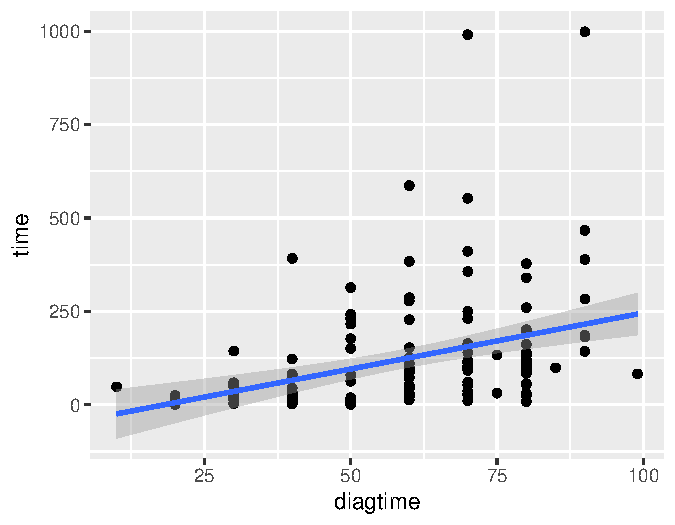
\includegraphics{R_BioST_book_files/figure-latex/unnamed-chunk-48-8.pdf}

\begin{Shaded}
\begin{Highlighting}[]
\KeywordTok{ggplot}\NormalTok{(}\DataTypeTok{data =}\NormalTok{ dd, }\KeywordTok{aes}\NormalTok{(}\DataTypeTok{x =}\NormalTok{ diagtime, }\DataTypeTok{y =}\NormalTok{ time)) }\OperatorTok{+}\StringTok{ }
\StringTok{  }\KeywordTok{geom\_point}\NormalTok{() }\OperatorTok{+}\StringTok{ }
\StringTok{  }\KeywordTok{geom\_smooth}\NormalTok{(}\DataTypeTok{se =} \OtherTok{FALSE}\NormalTok{)}
\end{Highlighting}
\end{Shaded}

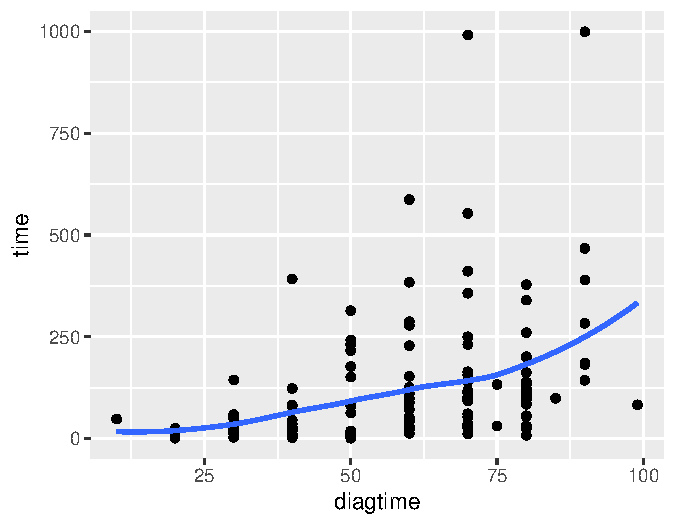
\includegraphics{R_BioST_book_files/figure-latex/unnamed-chunk-48-9.pdf}

\begin{Shaded}
\begin{Highlighting}[]
\KeywordTok{ggplot}\NormalTok{(}\DataTypeTok{data =}\NormalTok{ dd, }\KeywordTok{aes}\NormalTok{(}\DataTypeTok{x =}\NormalTok{ diagtime, }\DataTypeTok{y =}\NormalTok{ time)) }\OperatorTok{+}\StringTok{ }
\StringTok{  }\KeywordTok{geom\_point}\NormalTok{() }\OperatorTok{+}\StringTok{ }
\StringTok{  }\KeywordTok{geom\_smooth}\NormalTok{(}\DataTypeTok{method =} \StringTok{"lm"}\NormalTok{, }\DataTypeTok{se =} \OtherTok{FALSE}\NormalTok{) }\OperatorTok{+}\StringTok{ }
\StringTok{  }\KeywordTok{geom\_smooth}\NormalTok{(}\DataTypeTok{se =} \OtherTok{FALSE}\NormalTok{)}
\CommentTok{\#\# scatter plot + marginal distribution}
\KeywordTok{library}\NormalTok{(ggExtra)}
\CommentTok{\# classical}
\NormalTok{p \textless{}{-}}\StringTok{ }\KeywordTok{ggplot}\NormalTok{(dd, }\KeywordTok{aes}\NormalTok{(}\DataTypeTok{x =}\NormalTok{ diagtime, }\DataTypeTok{y =}\NormalTok{ time)) }\OperatorTok{+}
\StringTok{      }\KeywordTok{geom\_point}\NormalTok{() }\OperatorTok{+}
\StringTok{      }\KeywordTok{theme}\NormalTok{(}\DataTypeTok{legend.position =} \StringTok{"none"}\NormalTok{)}
\CommentTok{\# scatter plot + marginal histogram}
\KeywordTok{ggMarginal}\NormalTok{(p, }\DataTypeTok{type =} \StringTok{"histogram"}\NormalTok{, }\DataTypeTok{color =} \StringTok{"purple"}\NormalTok{)}
\CommentTok{\# scatter plot + marginal density}
\KeywordTok{ggMarginal}\NormalTok{(p, }\DataTypeTok{type =} \StringTok{"density"}\NormalTok{)}
\CommentTok{\# scatter plot + marginal boxplot}
\KeywordTok{ggMarginal}\NormalTok{(p, }\DataTypeTok{type =} \StringTok{"boxplot"}\NormalTok{)}
\end{Highlighting}
\end{Shaded}

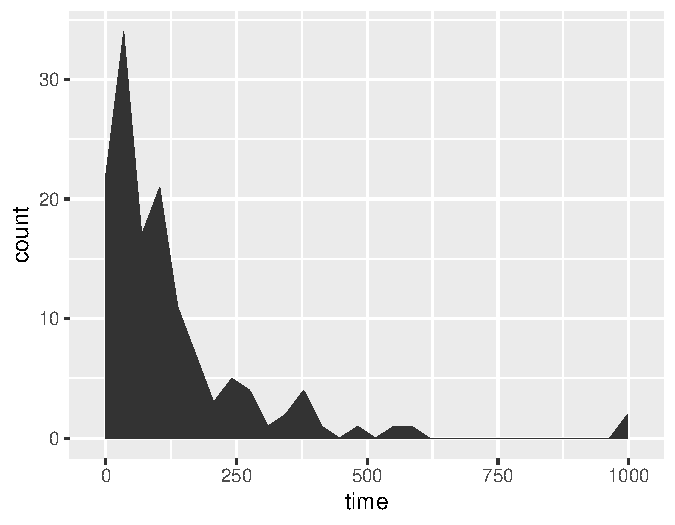
\includegraphics{R_BioST_book_files/figure-latex/unnamed-chunk-48-10.pdf}

\hypertarget{ux6df7ux5408ux8b8aux6578}{%
\section{混合變數}\label{ux6df7ux5408ux8b8aux6578}}

多變量視覺化分析

\begin{itemize}
\tightlist
\item
  一連續 + 一類別
\item
  二連續 + 一類別
\item
  二類別 + 一連續 = 一連續 + 一類別
\item
  多變數
\end{itemize}

\hypertarget{ux4e00ux9023ux7e8c-ux4e00ux985eux5225}{%
\subsection{一連續 + 一類別}\label{ux4e00ux9023ux7e8c-ux4e00ux985eux5225}}

\begin{Shaded}
\begin{Highlighting}[]
\CommentTok{\# one continuous + one categorical}
\KeywordTok{ggplot}\NormalTok{(}\DataTypeTok{data =}\NormalTok{ dd, }\KeywordTok{aes}\NormalTok{(}\DataTypeTok{x =}\NormalTok{ time)) }\OperatorTok{+}\StringTok{ }
\StringTok{  }\KeywordTok{geom\_histogram}\NormalTok{(}\KeywordTok{aes}\NormalTok{(}\DataTypeTok{fill =}\NormalTok{ treat))}
\end{Highlighting}
\end{Shaded}

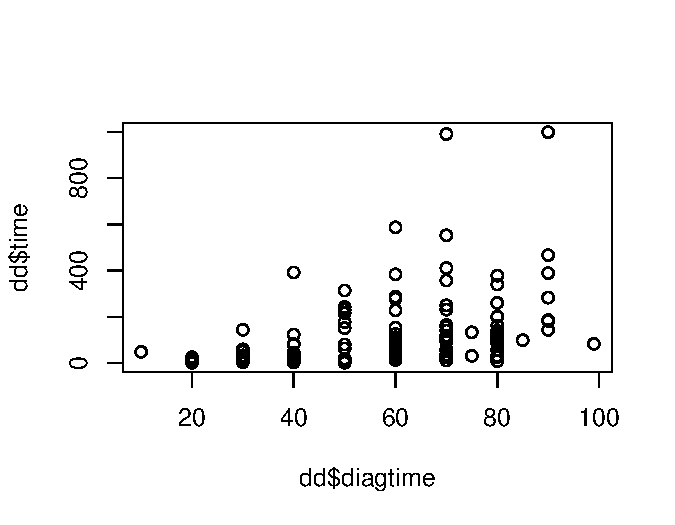
\includegraphics{R_BioST_book_files/figure-latex/unnamed-chunk-49-1.pdf}

\begin{Shaded}
\begin{Highlighting}[]
\KeywordTok{ggplot}\NormalTok{(}\DataTypeTok{data =}\NormalTok{ dd, }\KeywordTok{aes}\NormalTok{(}\DataTypeTok{x =}\NormalTok{ time, }\DataTypeTok{fill =}\NormalTok{ treat)) }\OperatorTok{+}
\StringTok{    }\KeywordTok{geom\_histogram}\NormalTok{( }\DataTypeTok{color =} \StringTok{"\#e9ecef"}\NormalTok{, }
                    \DataTypeTok{alpha =} \FloatTok{0.6}\NormalTok{, }
                    \DataTypeTok{position =} \StringTok{\textquotesingle{}identity\textquotesingle{}}\NormalTok{)}
\end{Highlighting}
\end{Shaded}

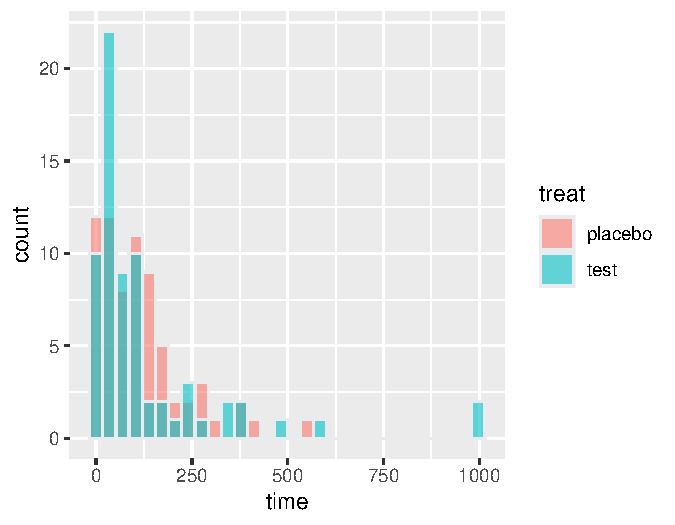
\includegraphics{R_BioST_book_files/figure-latex/unnamed-chunk-49-2.pdf}

\begin{Shaded}
\begin{Highlighting}[]
\KeywordTok{ggplot}\NormalTok{(}\DataTypeTok{data =}\NormalTok{ dd, }\KeywordTok{aes}\NormalTok{(}\DataTypeTok{x =}\NormalTok{ time, }\DataTypeTok{color =}\NormalTok{ treat, }\DataTypeTok{fill =}\NormalTok{ treat)) }\OperatorTok{+}
\StringTok{    }\KeywordTok{geom\_histogram}\NormalTok{()}
\end{Highlighting}
\end{Shaded}

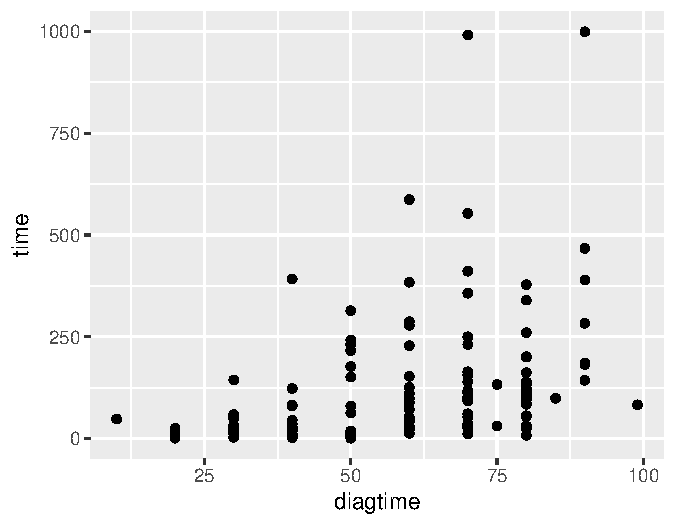
\includegraphics{R_BioST_book_files/figure-latex/unnamed-chunk-49-3.pdf}

\begin{Shaded}
\begin{Highlighting}[]
\CommentTok{\#}
\KeywordTok{ggplot}\NormalTok{(}\DataTypeTok{data =}\NormalTok{ dd, }\KeywordTok{aes}\NormalTok{(}\DataTypeTok{x =}\NormalTok{ treat, }\DataTypeTok{y =}\NormalTok{ time, }\DataTypeTok{fill =}\NormalTok{ treat)) }\OperatorTok{+}
\StringTok{    }\KeywordTok{geom\_boxplot}\NormalTok{()}
\end{Highlighting}
\end{Shaded}

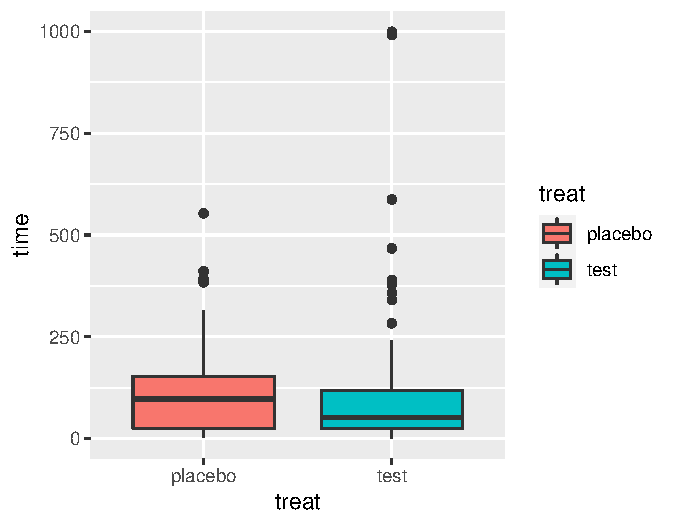
\includegraphics{R_BioST_book_files/figure-latex/unnamed-chunk-49-4.pdf}

\begin{Shaded}
\begin{Highlighting}[]
\KeywordTok{ggplot}\NormalTok{(}\DataTypeTok{data =}\NormalTok{ dd, }\KeywordTok{aes}\NormalTok{(}\DataTypeTok{x =}\NormalTok{ treat, }\DataTypeTok{y =}\NormalTok{ time, }\DataTypeTok{fill =}\NormalTok{ treat)) }\OperatorTok{+}
\StringTok{    }\KeywordTok{geom\_boxplot}\NormalTok{() }\OperatorTok{+}
\StringTok{    }\KeywordTok{geom\_jitter}\NormalTok{(}\DataTypeTok{color =} \StringTok{"purple"}\NormalTok{, }\DataTypeTok{size =} \DecValTok{2}\NormalTok{, }\DataTypeTok{alpha =} \FloatTok{0.8}\NormalTok{)}
\end{Highlighting}
\end{Shaded}

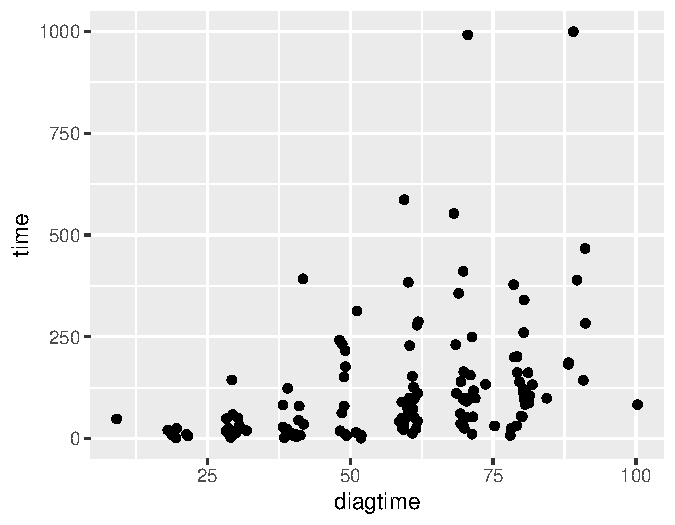
\includegraphics{R_BioST_book_files/figure-latex/unnamed-chunk-49-5.pdf}

\begin{Shaded}
\begin{Highlighting}[]
\CommentTok{\#}
\KeywordTok{ggplot}\NormalTok{(}\DataTypeTok{data =}\NormalTok{ dd, }\KeywordTok{aes}\NormalTok{(}\DataTypeTok{x =}\NormalTok{ treat, }\DataTypeTok{y =}\NormalTok{ time, }\DataTypeTok{fill =}\NormalTok{ treat)) }\OperatorTok{+}
\StringTok{    }\KeywordTok{geom\_violin}\NormalTok{()}
\end{Highlighting}
\end{Shaded}

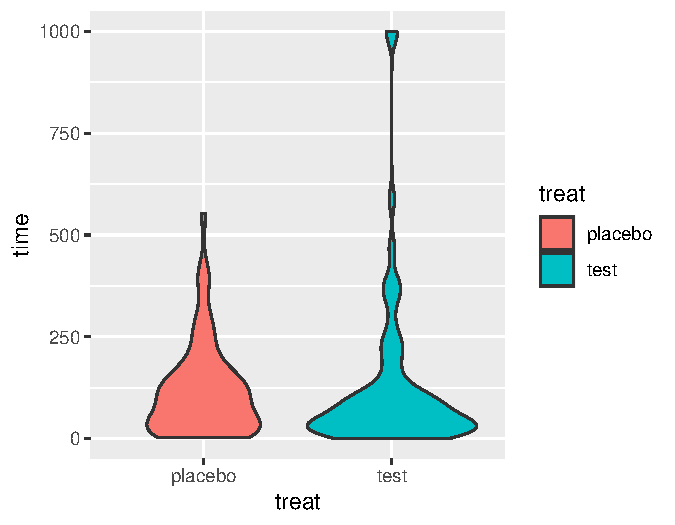
\includegraphics{R_BioST_book_files/figure-latex/unnamed-chunk-49-6.pdf}

\begin{Shaded}
\begin{Highlighting}[]
\KeywordTok{ggplot}\NormalTok{(}\DataTypeTok{data =}\NormalTok{ dd, }\KeywordTok{aes}\NormalTok{(}\DataTypeTok{x =}\NormalTok{ treat, }\DataTypeTok{y =}\NormalTok{ time, }\DataTypeTok{fill =}\NormalTok{ treat)) }\OperatorTok{+}
\StringTok{    }\KeywordTok{geom\_violin}\NormalTok{() }\OperatorTok{+}
\StringTok{    }\KeywordTok{geom\_jitter}\NormalTok{(}\DataTypeTok{color =} \StringTok{"purple"}\NormalTok{, }\DataTypeTok{size =} \DecValTok{2}\NormalTok{, }\DataTypeTok{alpha =} \FloatTok{0.8}\NormalTok{) }\OperatorTok{+}\StringTok{ }
\StringTok{  }\KeywordTok{ggtitle}\NormalTok{(}\StringTok{"Violin chart by treatment"}\NormalTok{) }\OperatorTok{+}
\StringTok{    }\KeywordTok{xlab}\NormalTok{(}\StringTok{"treatment"}\NormalTok{)}
\end{Highlighting}
\end{Shaded}

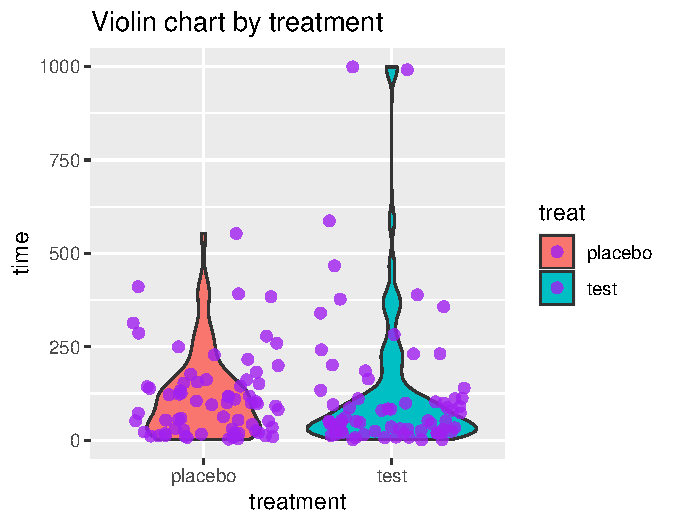
\includegraphics{R_BioST_book_files/figure-latex/unnamed-chunk-49-7.pdf}

\hypertarget{ux4e8cux9023ux7e8c-ux4e00ux985eux5225}{%
\subsection{二連續 + 一類別}\label{ux4e8cux9023ux7e8c-ux4e00ux985eux5225}}

\begin{Shaded}
\begin{Highlighting}[]
\CommentTok{\#\# ggplot2}
\CommentTok{\#\# two continuous + one categorical}
\KeywordTok{ggplot}\NormalTok{(}\DataTypeTok{data =}\NormalTok{ dd, }\KeywordTok{aes}\NormalTok{(}\DataTypeTok{x =}\NormalTok{ diagtime, }\DataTypeTok{y =}\NormalTok{ time, }\DataTypeTok{color =}\NormalTok{ treat)) }\OperatorTok{+}\StringTok{ }
\StringTok{  }\KeywordTok{geom\_point}\NormalTok{(}\DataTypeTok{size =} \DecValTok{4}\NormalTok{)}
\end{Highlighting}
\end{Shaded}

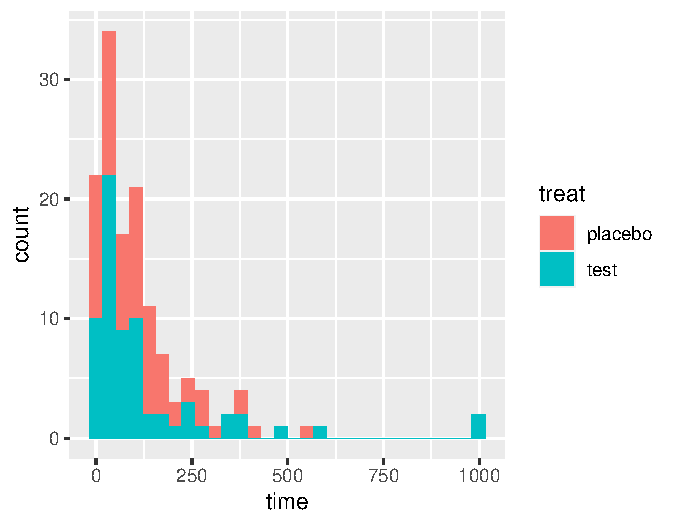
\includegraphics{R_BioST_book_files/figure-latex/unnamed-chunk-50-1.pdf}

\begin{Shaded}
\begin{Highlighting}[]
\KeywordTok{ggplot}\NormalTok{(}\DataTypeTok{data =}\NormalTok{ dd, }\KeywordTok{aes}\NormalTok{(}\DataTypeTok{x =}\NormalTok{ diagtime, }\DataTypeTok{y =}\NormalTok{ time, }\DataTypeTok{color =}\NormalTok{ treat)) }\OperatorTok{+}\StringTok{ }
\StringTok{  }\KeywordTok{geom\_jitter}\NormalTok{(}\DataTypeTok{size =} \DecValTok{4}\NormalTok{)}
\end{Highlighting}
\end{Shaded}

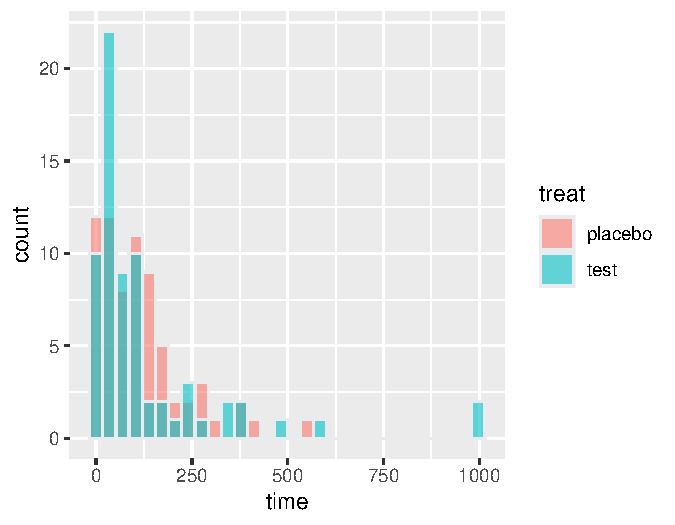
\includegraphics{R_BioST_book_files/figure-latex/unnamed-chunk-50-2.pdf}

\begin{Shaded}
\begin{Highlighting}[]
\KeywordTok{ggplot}\NormalTok{(}\DataTypeTok{data =}\NormalTok{ dd, }\KeywordTok{aes}\NormalTok{(}\DataTypeTok{x =}\NormalTok{ diagtime, }\DataTypeTok{y =}\NormalTok{ time, }
                      \DataTypeTok{color =}\NormalTok{ treat, }\DataTypeTok{shape =}\NormalTok{ treat, }\DataTypeTok{size =}\NormalTok{ treat)) }\OperatorTok{+}\StringTok{ }
\StringTok{  }\KeywordTok{geom\_jitter}\NormalTok{(}\DataTypeTok{alpha =} \DecValTok{1}\OperatorTok{/}\DecValTok{2}\NormalTok{) }
\end{Highlighting}
\end{Shaded}

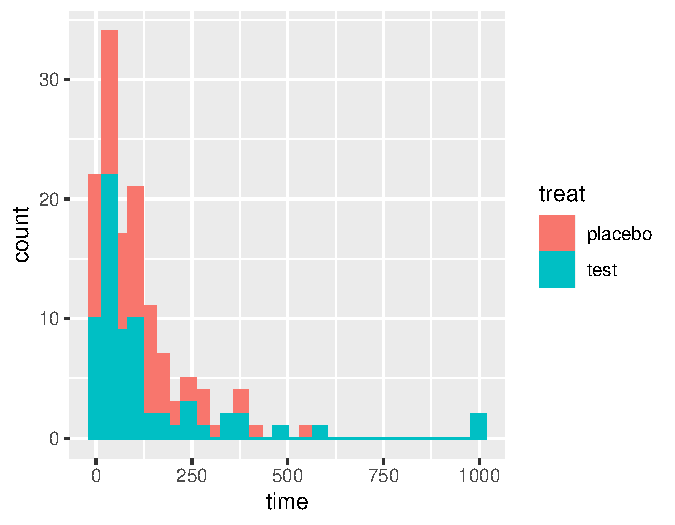
\includegraphics{R_BioST_book_files/figure-latex/unnamed-chunk-50-3.pdf}

\begin{Shaded}
\begin{Highlighting}[]
\CommentTok{\# add linear line or smoothing line}
\KeywordTok{ggplot}\NormalTok{(}\DataTypeTok{data =}\NormalTok{ dd, }\KeywordTok{aes}\NormalTok{(}\DataTypeTok{x =}\NormalTok{ diagtime, }\DataTypeTok{y =}\NormalTok{ time, }
                      \DataTypeTok{color =}\NormalTok{ treat, }\DataTypeTok{shape =}\NormalTok{ treat)) }\OperatorTok{+}\StringTok{ }
\StringTok{  }\KeywordTok{geom\_point}\NormalTok{() }\OperatorTok{+}\StringTok{ }
\StringTok{  }\KeywordTok{geom\_smooth}\NormalTok{(}\DataTypeTok{method =} \StringTok{"lm"}\NormalTok{)}
\end{Highlighting}
\end{Shaded}

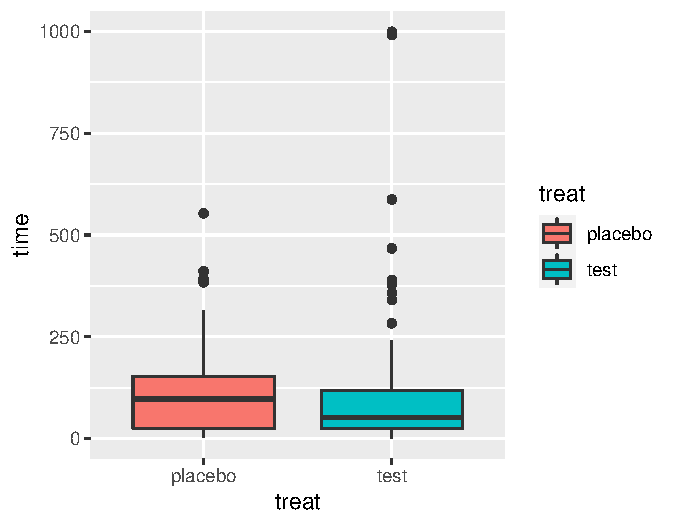
\includegraphics{R_BioST_book_files/figure-latex/unnamed-chunk-50-4.pdf}

\begin{Shaded}
\begin{Highlighting}[]
\KeywordTok{ggplot}\NormalTok{(}\DataTypeTok{data =}\NormalTok{ dd, }\KeywordTok{aes}\NormalTok{(}\DataTypeTok{x =}\NormalTok{ diagtime, }\DataTypeTok{y =}\NormalTok{ time, }
                      \DataTypeTok{color =}\NormalTok{ treat, }\DataTypeTok{shape =}\NormalTok{ treat)) }\OperatorTok{+}\StringTok{ }
\StringTok{  }\KeywordTok{geom\_point}\NormalTok{() }\OperatorTok{+}\StringTok{ }
\StringTok{  }\KeywordTok{geom\_smooth}\NormalTok{(}\DataTypeTok{method =} \StringTok{"lm"}\NormalTok{, }\DataTypeTok{se =} \OtherTok{FALSE}\NormalTok{)}
\end{Highlighting}
\end{Shaded}

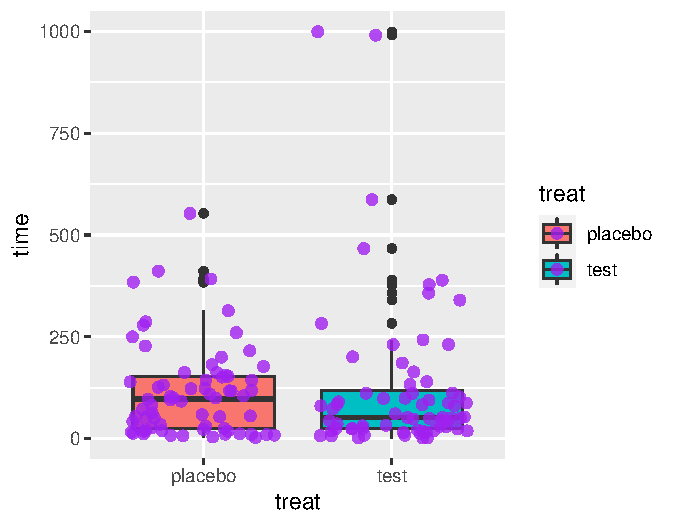
\includegraphics{R_BioST_book_files/figure-latex/unnamed-chunk-50-5.pdf}

\begin{Shaded}
\begin{Highlighting}[]
\CommentTok{\#}
\KeywordTok{ggplot}\NormalTok{(}\DataTypeTok{data =}\NormalTok{ dd, }\KeywordTok{aes}\NormalTok{(}\DataTypeTok{x =}\NormalTok{ diagtime, }\DataTypeTok{y =}\NormalTok{ time,}
                      \DataTypeTok{color =}\NormalTok{ treat, }\DataTypeTok{shape =}\NormalTok{ treat)) }\OperatorTok{+}\StringTok{ }
\StringTok{  }\KeywordTok{geom\_point}\NormalTok{() }\OperatorTok{+}\StringTok{ }
\StringTok{  }\KeywordTok{geom\_smooth}\NormalTok{(}\DataTypeTok{se =} \OtherTok{FALSE}\NormalTok{)}
\end{Highlighting}
\end{Shaded}

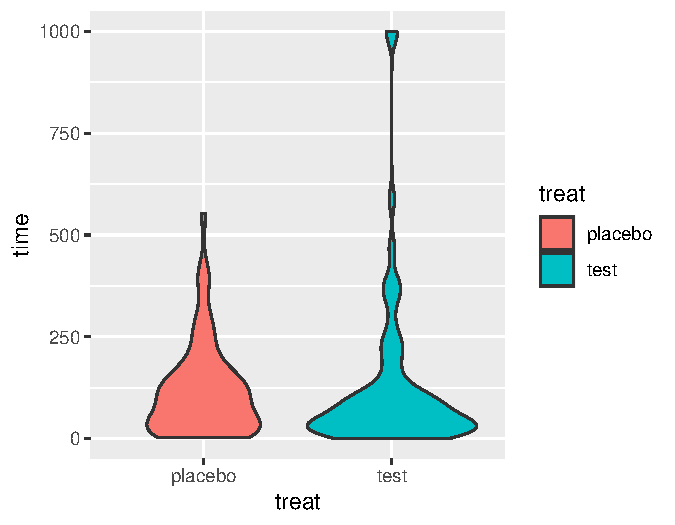
\includegraphics{R_BioST_book_files/figure-latex/unnamed-chunk-50-6.pdf}

\begin{Shaded}
\begin{Highlighting}[]
\CommentTok{\# BAD! too many lines}
\KeywordTok{ggplot}\NormalTok{(}\DataTypeTok{data =}\NormalTok{ dd, }\KeywordTok{aes}\NormalTok{(}\DataTypeTok{x =}\NormalTok{ diagtime, }\DataTypeTok{y =}\NormalTok{ time,}
                      \DataTypeTok{color =}\NormalTok{ treat, }\DataTypeTok{shape =}\NormalTok{ treat)) }\OperatorTok{+}\StringTok{ }
\StringTok{  }\KeywordTok{geom\_point}\NormalTok{() }\OperatorTok{+}\StringTok{ }
\StringTok{  }\KeywordTok{geom\_smooth}\NormalTok{(}\DataTypeTok{method =} \StringTok{"lm"}\NormalTok{, }\DataTypeTok{se =} \OtherTok{FALSE}\NormalTok{) }\OperatorTok{+}\StringTok{ }
\StringTok{  }\KeywordTok{geom\_smooth}\NormalTok{(}\DataTypeTok{se =} \OtherTok{FALSE}\NormalTok{)}
\CommentTok{\# classical}
\NormalTok{p \textless{}{-}}\StringTok{ }\KeywordTok{ggplot}\NormalTok{(dd, }\KeywordTok{aes}\NormalTok{(}\DataTypeTok{x =}\NormalTok{ diagtime, }\DataTypeTok{y =}\NormalTok{ time, }\DataTypeTok{color =}\NormalTok{ treat)) }\OperatorTok{+}
\StringTok{      }\KeywordTok{geom\_point}\NormalTok{(}\DataTypeTok{size =} \DecValTok{5}\NormalTok{) }
\CommentTok{\# scatter plot + marginal histogram}
\NormalTok{ggExtra}\OperatorTok{::}\KeywordTok{ggMarginal}\NormalTok{(p, }\DataTypeTok{type =} \StringTok{"histogram"}\NormalTok{, }\DataTypeTok{color =} \StringTok{"purple"}\NormalTok{)}
\end{Highlighting}
\end{Shaded}

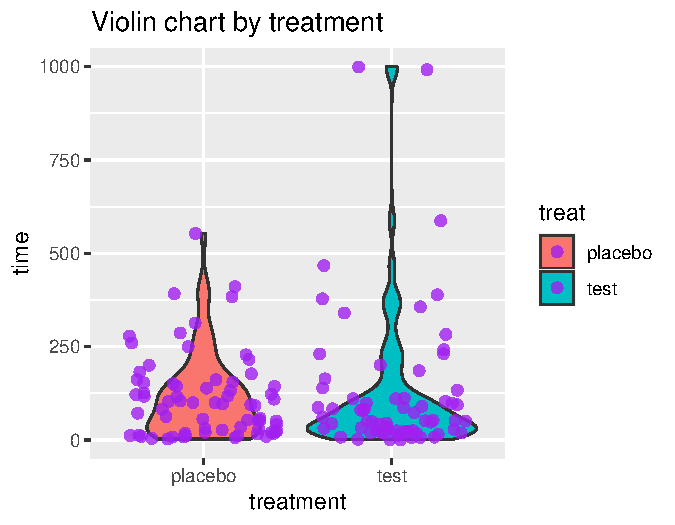
\includegraphics{R_BioST_book_files/figure-latex/unnamed-chunk-50-7.pdf}

\hypertarget{ux4e09ux9023ux7e8cux8b8aux6578}{%
\subsection{三連續變數}\label{ux4e09ux9023ux7e8cux8b8aux6578}}

\begin{itemize}
\tightlist
\item
  多連續變數: 檢視成對變數關聯性, 大小, 方向, 趨勢.
\end{itemize}

\begin{Shaded}
\begin{Highlighting}[]
\CommentTok{\#\# pairwise scatter plot}
\CommentTok{\#\# R base}
\NormalTok{con.df =}\StringTok{ }\NormalTok{dd[, }\KeywordTok{c}\NormalTok{(}\StringTok{"time"}\NormalTok{, }\StringTok{"diagtime"}\NormalTok{, }\StringTok{"kps"}\NormalTok{, }\StringTok{"age"}\NormalTok{)]}
\NormalTok{cor.mat =}\StringTok{ }\KeywordTok{cor}\NormalTok{(con.df, }\DataTypeTok{use =} \StringTok{"complete"}\NormalTok{, }\DataTypeTok{method =} \StringTok{"pearson"}\NormalTok{)}
\KeywordTok{round}\NormalTok{(cor.mat, }\DecValTok{3}\NormalTok{)}
\CommentTok{\#\#            time diagtime    kps    age}
\CommentTok{\#\# time      1.000    0.382 {-}0.046 {-}0.068}
\CommentTok{\#\# diagtime  0.382    1.000 {-}0.184 {-}0.095}
\CommentTok{\#\# kps      {-}0.046   {-}0.184  1.000 {-}0.033}
\CommentTok{\#\# age      {-}0.068   {-}0.095 {-}0.033  1.000}
\KeywordTok{pairs}\NormalTok{(con.df)}
\end{Highlighting}
\end{Shaded}

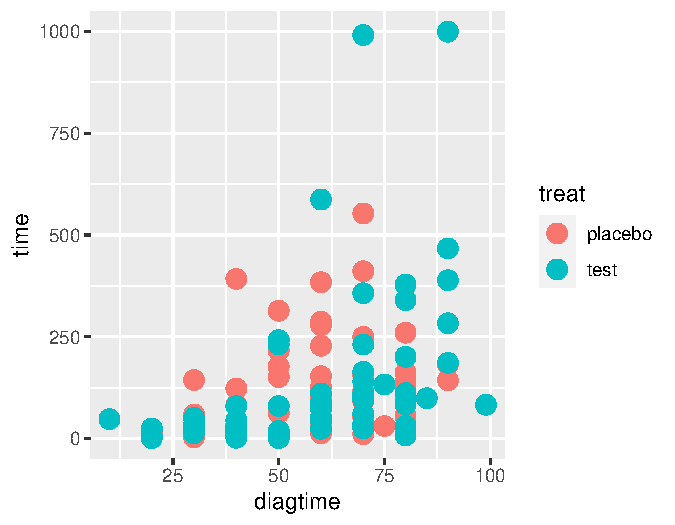
\includegraphics{R_BioST_book_files/figure-latex/unnamed-chunk-51-1.pdf}

\begin{Shaded}
\begin{Highlighting}[]
\CommentTok{\#\# ggplot2}
\KeywordTok{library}\NormalTok{(GGally)}
\NormalTok{GGally}\OperatorTok{::}\KeywordTok{ggpairs}\NormalTok{(}\DataTypeTok{data =}\NormalTok{ con.df)}
\end{Highlighting}
\end{Shaded}

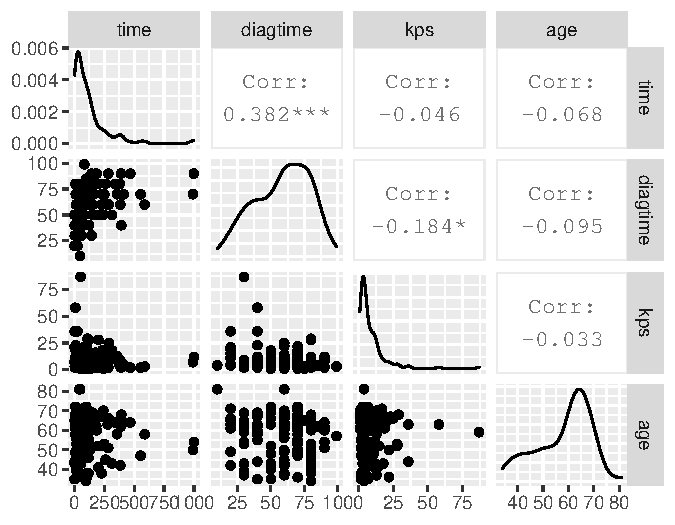
\includegraphics{R_BioST_book_files/figure-latex/unnamed-chunk-51-2.pdf}

\begin{Shaded}
\begin{Highlighting}[]
\NormalTok{GGally}\OperatorTok{::}\KeywordTok{ggcorr}\NormalTok{(}\DataTypeTok{data =}\NormalTok{ con.df, }
               \DataTypeTok{method =} \KeywordTok{c}\NormalTok{(}\StringTok{"complete"}\NormalTok{, }\StringTok{"pearson"}\NormalTok{))}
\end{Highlighting}
\end{Shaded}

\includegraphics{R_BioST_book_files/figure-latex/unnamed-chunk-51-3.pdf}

\begin{Shaded}
\begin{Highlighting}[]
\CommentTok{\#\# Correlogram}
\KeywordTok{library}\NormalTok{(corrgram)}
\KeywordTok{corrgram}\NormalTok{(}\DataTypeTok{x =}\NormalTok{ dd, }
         \DataTypeTok{order =} \OtherTok{TRUE}\NormalTok{, }
         \DataTypeTok{lower.panel =}\NormalTok{ panel.shade, }
         \DataTypeTok{upper.panel =}\NormalTok{ panel.pie, }
         \DataTypeTok{text.panel =}\NormalTok{ panel.txt, }
         \DataTypeTok{main =} \StringTok{"1. VA Lung Cancer Trial"}\NormalTok{)}
\end{Highlighting}
\end{Shaded}

\includegraphics{R_BioST_book_files/figure-latex/unnamed-chunk-51-4.pdf}

\begin{Shaded}
\begin{Highlighting}[]
\KeywordTok{corrgram}\NormalTok{(}\DataTypeTok{x =}\NormalTok{ dd, }
         \DataTypeTok{order =} \OtherTok{TRUE}\NormalTok{, }
         \DataTypeTok{lower.panel =}\NormalTok{ panel.ellipse, }
         \DataTypeTok{upper.panel =}\NormalTok{ panel.pts, }
         \DataTypeTok{text.panel =}\NormalTok{ panel.minmax, }
         \DataTypeTok{main =} \StringTok{"2. VA Lung Cancer Trial"}\NormalTok{)}
\end{Highlighting}
\end{Shaded}

\includegraphics{R_BioST_book_files/figure-latex/unnamed-chunk-51-5.pdf}

\begin{Shaded}
\begin{Highlighting}[]
\KeywordTok{corrgram}\NormalTok{(}\DataTypeTok{x =}\NormalTok{ dd, }
         \DataTypeTok{order =} \OtherTok{NULL}\NormalTok{, }
         \DataTypeTok{lower.panel =}\NormalTok{ panel.shade, }
         \DataTypeTok{upper.panel =} \OtherTok{NULL}\NormalTok{, }
         \DataTypeTok{text.panel =}\NormalTok{ panel.txt, }
         \DataTypeTok{main =} \StringTok{"3. VA Lung Cancer Trial"}\NormalTok{)}
\end{Highlighting}
\end{Shaded}

\includegraphics{R_BioST_book_files/figure-latex/unnamed-chunk-51-6.pdf}

\begin{itemize}
\tightlist
\item
  Try by yourself!
\end{itemize}

\begin{Shaded}
\begin{Highlighting}[]
\CommentTok{\# more advanced}
\NormalTok{my\_fn \textless{}{-}}\StringTok{ }\ControlFlowTok{function}\NormalTok{(data, mapping, ...)\{}
\NormalTok{  p \textless{}{-}}\StringTok{ }\KeywordTok{ggplot}\NormalTok{(}\DataTypeTok{data =}\NormalTok{ data, }\DataTypeTok{mapping =}\NormalTok{ mapping) }\OperatorTok{+}\StringTok{ }
\StringTok{    }\KeywordTok{geom\_point}\NormalTok{() }\OperatorTok{+}\StringTok{ }
\StringTok{    }\KeywordTok{geom\_smooth}\NormalTok{(}\DataTypeTok{method =}\NormalTok{ loess, }\DataTypeTok{se =} \OtherTok{FALSE}\NormalTok{, }\DataTypeTok{fill =} \StringTok{"red"}\NormalTok{, }\DataTypeTok{treat =} \StringTok{"red"}\NormalTok{, ...) }\OperatorTok{+}
\StringTok{    }\KeywordTok{geom\_smooth}\NormalTok{(}\DataTypeTok{method =}\NormalTok{ lm, }\DataTypeTok{se =} \OtherTok{FALSE}\NormalTok{, }\DataTypeTok{fill =} \StringTok{"blue"}\NormalTok{, }\DataTypeTok{treat =} \StringTok{"blue"}\NormalTok{, ...)}
\NormalTok{  p}
\NormalTok{\}}
\NormalTok{GGally}\OperatorTok{::}\KeywordTok{ggpairs}\NormalTok{(}\DataTypeTok{data =}\NormalTok{ con.df, }
        \DataTypeTok{lower =} \KeywordTok{list}\NormalTok{(}\DataTypeTok{continuous =}\NormalTok{ my\_fn))}
\end{Highlighting}
\end{Shaded}

\includegraphics{R_BioST_book_files/figure-latex/unnamed-chunk-52-1.pdf}

\begin{Shaded}
\begin{Highlighting}[]
\CommentTok{\#\# Bubble plot}
\KeywordTok{ggplot}\NormalTok{(}\DataTypeTok{data =}\NormalTok{ dd, }\KeywordTok{aes}\NormalTok{(}\DataTypeTok{x =}\NormalTok{ diagtime, }\DataTypeTok{y =}\NormalTok{ time, }\DataTypeTok{size =}\NormalTok{ age)) }\OperatorTok{+}\StringTok{ }
\StringTok{  }\KeywordTok{geom\_point}\NormalTok{(}\DataTypeTok{alpha =} \FloatTok{0.3}\NormalTok{) }\OperatorTok{+}\StringTok{ }
\StringTok{  }\KeywordTok{scale\_size}\NormalTok{(}\DataTypeTok{range =} \KeywordTok{c}\NormalTok{(.}\DecValTok{1}\NormalTok{, }\DecValTok{15}\NormalTok{), }\DataTypeTok{name=}\StringTok{"Age Bubbles"}\NormalTok{)}
\end{Highlighting}
\end{Shaded}

\includegraphics{R_BioST_book_files/figure-latex/unnamed-chunk-53-1.pdf}

\begin{Shaded}
\begin{Highlighting}[]
\KeywordTok{ggplot}\NormalTok{(}\DataTypeTok{data =}\NormalTok{ dd, }\KeywordTok{aes}\NormalTok{(}\DataTypeTok{x =}\NormalTok{ diagtime, }\DataTypeTok{y =}\NormalTok{ time, }\DataTypeTok{size =}\NormalTok{ age)) }\OperatorTok{+}\StringTok{ }
\StringTok{  }\KeywordTok{geom\_point}\NormalTok{(}\DataTypeTok{alpha =} \FloatTok{0.3}\NormalTok{) }\OperatorTok{+}\StringTok{ }
\StringTok{  }\KeywordTok{scale\_size}\NormalTok{(}\DataTypeTok{range =} \KeywordTok{c}\NormalTok{(.}\DecValTok{1}\NormalTok{, }\DecValTok{15}\NormalTok{), }\DataTypeTok{name=}\StringTok{"Age Bubbles"}\NormalTok{)}
\end{Highlighting}
\end{Shaded}

\includegraphics{R_BioST_book_files/figure-latex/unnamed-chunk-53-2.pdf}

\begin{Shaded}
\begin{Highlighting}[]
\KeywordTok{ggplot}\NormalTok{(}\DataTypeTok{data =}\NormalTok{ dd, }\KeywordTok{aes}\NormalTok{(}\DataTypeTok{x =}\NormalTok{ diagtime, }\DataTypeTok{y =}\NormalTok{ time, }\DataTypeTok{size =}\NormalTok{ age, }\DataTypeTok{color =}\NormalTok{ treat)) }\OperatorTok{+}\StringTok{ }
\StringTok{  }\KeywordTok{geom\_point}\NormalTok{(}\DataTypeTok{alpha =} \FloatTok{0.3}\NormalTok{) }\OperatorTok{+}\StringTok{ }
\KeywordTok{scale\_size}\NormalTok{(}\DataTypeTok{range =} \KeywordTok{c}\NormalTok{(.}\DecValTok{1}\NormalTok{, }\DecValTok{24}\NormalTok{), }\DataTypeTok{name =} \StringTok{""}\NormalTok{)}
\end{Highlighting}
\end{Shaded}

\includegraphics{R_BioST_book_files/figure-latex/unnamed-chunk-53-3.pdf}

\hypertarget{ux5206ux7d44ux7e6aux5716}{%
\section{分組繪圖}\label{ux5206ux7d44ux7e6aux5716}}

\begin{itemize}
\tightlist
\item
  將資料依據組別分割成子資料集
\item
  將每個子資料集繪製在不同的圖格
\item
  將所有子資料集的圖格合併呈現
\end{itemize}

\begin{Shaded}
\begin{Highlighting}[]
\CommentTok{\# plot by treat}
\KeywordTok{ggplot}\NormalTok{(}\DataTypeTok{data =}\NormalTok{ dd, }\KeywordTok{aes}\NormalTok{(}\DataTypeTok{x =}\NormalTok{ diagtime, }\DataTypeTok{y =}\NormalTok{ time)) }\OperatorTok{+}\StringTok{ }\KeywordTok{geom\_jitter}\NormalTok{() }\OperatorTok{+}\StringTok{ }
\StringTok{  }\KeywordTok{facet\_grid}\NormalTok{(. }\OperatorTok{\textasciitilde{}}\StringTok{ }\NormalTok{treat)}
\end{Highlighting}
\end{Shaded}

\includegraphics{R_BioST_book_files/figure-latex/unnamed-chunk-54-1.pdf}

\begin{Shaded}
\begin{Highlighting}[]
\KeywordTok{ggplot}\NormalTok{(}\DataTypeTok{data =}\NormalTok{ dd, }\KeywordTok{aes}\NormalTok{(}\DataTypeTok{x =}\NormalTok{ diagtime, }\DataTypeTok{y =}\NormalTok{ time)) }\OperatorTok{+}\StringTok{ }\KeywordTok{geom\_jitter}\NormalTok{() }\OperatorTok{+}\StringTok{ }
\StringTok{  }\KeywordTok{facet\_grid}\NormalTok{(treat }\OperatorTok{\textasciitilde{}}\StringTok{ }\NormalTok{.)}
\end{Highlighting}
\end{Shaded}

\includegraphics{R_BioST_book_files/figure-latex/unnamed-chunk-54-2.pdf}

\begin{Shaded}
\begin{Highlighting}[]
\CommentTok{\# plot by cellcode}
\KeywordTok{ggplot}\NormalTok{(}\DataTypeTok{data =}\NormalTok{ dd, }\KeywordTok{aes}\NormalTok{(}\DataTypeTok{x =}\NormalTok{ diagtime, }\DataTypeTok{y =}\NormalTok{ time)) }\OperatorTok{+}\StringTok{ }\KeywordTok{geom\_jitter}\NormalTok{() }\OperatorTok{+}\StringTok{ }
\StringTok{  }\KeywordTok{facet\_grid}\NormalTok{(. }\OperatorTok{\textasciitilde{}}\StringTok{ }\NormalTok{cellcode)}
\end{Highlighting}
\end{Shaded}

\includegraphics{R_BioST_book_files/figure-latex/unnamed-chunk-54-3.pdf}

\begin{Shaded}
\begin{Highlighting}[]
\CommentTok{\# two factors}
\KeywordTok{ggplot}\NormalTok{(}\DataTypeTok{data =}\NormalTok{ dd, }\KeywordTok{aes}\NormalTok{(}\DataTypeTok{x =}\NormalTok{ diagtime, }\DataTypeTok{y =}\NormalTok{ time)) }\OperatorTok{+}\StringTok{ }\KeywordTok{geom\_jitter}\NormalTok{() }\OperatorTok{+}\StringTok{ }
\StringTok{  }\KeywordTok{facet\_grid}\NormalTok{(treat }\OperatorTok{\textasciitilde{}}\StringTok{ }\NormalTok{cellcode)}
\end{Highlighting}
\end{Shaded}

\includegraphics{R_BioST_book_files/figure-latex/unnamed-chunk-54-4.pdf}

  \bibliography{book.bib,packages.bib}

\end{document}
